\documentclass{article}
\usepackage{xcolor}
\usepackage{minted}
\usepackage{multicol}

% Author info %
\title{AQA A Level Computer Science NEA}
\date{2023}
\author{Luka Warren}

% Code snippet config %
\setminted{fontsize=\footnotesize}

% For images %
\usepackage{graphicx}
\graphicspath{{images/}}

% Page layout %
\usepackage[margin=1.0in]{geometry}
\setlength{\fboxsep}{1.5em}
\addtolength{\footnotesep}{5mm}
\usepackage[hang]{footmisc}
\setlength{\footnotemargin}{4mm}

% Make table of contents have link to the pages %
\usepackage{hyperref}
\hypersetup{
	colorlinks,
	citecolor=black,
	filecolor=black,
	linkcolor=black,
	urlcolor=black
}

% Fix quotes %
\usepackage [english]{babel}
\usepackage [autostyle, english = american]{csquotes}
\MakeOuterQuote{"}

% Allow use of text in MathJax
\usepackage{amsmath}

% Tables %
\usepackage{tabularx}

\begin{document}

	% Title page %
	\maketitle
	\pagenumbering{gobble}
	\tableofcontents
	\newpage
	\pagenumbering{arabic}

	% Page breaks %
	\AddToHook{cmd/section/before}{\clearpage}
	% \AddToHook{cmd/subsection/before}{\clearpage} %

	\section{Analysis}

\subsection{Background}
There exists online many popular "remixes"  where someone has taken an existing song and distorted it, usually by adjusting its speed, bass and pitch, to achieve a desired effect. Often these versions of the song are preferred to the originals when used to accompany short-form content on video-sharing sites such as TikTok. For example,  the song "Money Trees" by Kendrick Lamar has 120 million views on YouTube  in its original form, but also a sizeable 1.6 million views on one "TikTok remix" alone, and indeed on TikTok itself it is rare to hear the original version. This pattern is also observed on other short-form video content sites, such as Instagram Reels and YouTube Shorts.

\paragraph{}
As such it can be seen that there exists a large audience of people who enjoy listening to altered versions of popular songs. However, the most popular music listening programs, including Spotify and YouTube music, provide no mechanism for manually altering songs by one's self. Instead, "remixes" must be created in external audio editing programs. Thus if a user wants to create their own "remixes", a unique issue is presented:
\begin{itemize}
	\item Suppose, for example, that a user wants to listen to a selection of songs, but sped-up and with a bass-boost applied, as is typical for song "remixes" on TikTok. Many songs do not have any accompanying "remixes" to satisfy this user's need, so they wish to do things themselves.
	\item As there exists no mainstream solution to edit music in real-time, the user would have to import their music files into an audio editing program and apply any desired effects to each file. This will take considerable time.
	\item However, what if the user then wishes to change the intensity or nature of the effects applied?
	\item Unfortunately now, they would have to repeat the entire audio-editing process again, waiting considerable time before the results of their experimentation could be heard (as one's entire music collection would thus have to be "remixed" again)
	\item The barrier for entry for creating and experimenting with different audio effects for large catalogues of music is thus considerable. One cannot quickly decide to turn up the bass or add an echo, for example, without opening an external program and interrupting playback.
	\item Easy and user-friendly experimentation is hence prevented, limiting the number of people willing to try editing audio, and hence the number of remixes that exist.
\end{itemize}

\paragraph{}
It is therefore the aim of this coursework to create a system to allow users to "remix" songs in real-time as they listen to them. In other words, the goal is to create a program that can not only play a user's music, but also allow them to edit it live, removing the need for external program and allowing them to tweaks audio effects instantly, without delay. Such a system would allow for comprehensible, user-friendly experimentation, removing the above barrier to entry and providing greater convenience.

\paragraph{}
However, a system can only be comprehensible and user-friendly if the exact needs of the users themselves are known, and so first a representative sub-section of the user-base must be interviewed.

\pagebreak
\subsection{Collection of Data}
\paragraph{}
A number of interviews were conducted with peers that self-reported to enjoy listening to song "remixes". The full interview form can be seen in the appendix. Below are the responses collected from my peers, which I believe represents the target demographic for this software, as those who listen to song remixes, particularly on TikTok, are typically of my age.

\paragraph{}
These responses have been "tidied up" by formatting them within the rest of the document for the benefit of the reader. However, the "raw screenshots" can be viewed in the appendix under "Questionnaire Responses" if such formatting proves confusing.

\subsubsection{Student 1}
{
\centering
\fbox{\begin{minipage}{15cm}
		\begin{center}
			{\huge Luka's Questionnaire Form}
		\end{center}
		
		For my A-level Computer Science coursework  I am writing a program that allows users to easily apply various audio effects to live songs, in order to make experimenting with music and creating remixes easier. In other words, I am writing a program where you can "remix" music as you listen to it, so that experimentation can be done quickly and without hassle. In order to create the best possible software, I would like your opinion on what makes a remix good, and what features you would expect my software to have. Please answer the questions below then email me your responses.
		
		\paragraph{Questions}
		\begin{enumerate}
			\item Why do you sometimes prefer a song's remix?
			\item How does a remix typically differ from the original song?
			\item My program is meant to lower the barrier of entry for editing audio as much as possible. How can I further enhance ease-of-use?
			\item Are there any other features  you would like in a real-time audio editing program to assist in "remixing" music?
			\item How do you currently listen to music?
		\end{enumerate}
		
		\paragraph{Responses:}
		\begin{enumerate}
			\item Videos on TikTok are only about 30 seconds long. It's good to speed up a song because otherwise you couldn't enjoy the full chorus. I also think music played at different speeds makes it sound new and more interesting.
			\item It's usually faster or slower, and people like to change the bass as well so it sounds better.
			\item I've tried editing audio before but I always get confused with all the options. I like the idea of it being live because then I can instantly hear what difference my choices are making. But if I had to pick one new feature, I'd want one of those music visualisations as well. It's always very easy to understand if a song has lots of bass, for example, because you can see the bass being visualised. If I was doing things like changing the bass, being able to see this change (as well as hear it) would be really useful.
			\item In Spotify there are presets for the equaliser where you can quickly choose, for example, if you want a "bass boost" preset of a "vocal boost" preset. I like the idea of being able to quickly chose a pre-defined set of options to eliminate the hassle of doing it manually - especially if I'm unsure of how to use the software to its fullest potential just yet!
			\item I use Spotify. You can't do any audio editing in that though. It's a shame I can't change the speed.
		\end{enumerate}
		\bigskip \bigskip \bigskip
\end{minipage}}
}

\pagebreak
\subsubsection{Student 2}
{
	\centering
	\fbox{\begin{minipage}{15cm}
			\begin{center}
				{\huge Luka's Questionnaire Form}
			\end{center}
			
			For my A-level Computer Science coursework  I am writing a program that allows users to easily apply various audio effects to live songs, in order to make experimenting with music and creating remixes easier. In other words, I am writing a program where you can "remix" music as you listen to it, so that experimentation can be done quickly and without hassle. In order to create the best possible software, I would like your opinion on what makes a remix good, and what features you would expect my software to have. Please answer the questions below then email me your responses.
			
			\paragraph{Questions}
			\begin{enumerate}
				\item Why do you sometimes prefer a song's remix?
				\item How does a remix typically differ from the original song?
				\item My program is meant to lower the barrier of entry for editing audio as much as possible. How can I further enhance ease-of-use?
				\item Are there any other features  you would like in a real-time audio editing program to assist in "remixing" music?
				\item How do you currently listen to music?
			\end{enumerate}
			
			\paragraph{Responses:}
			\begin{enumerate}
				\item I get bored listening to the same songs over and over, but hearing a remix makes it sound new and exciting.
				\item Usually there's a small echo that's added (I think it's called reverb). Also there's these crackles that get added to Lo-Fi music called noise that I think makes music quite calming. I'd really like to be able to add noise to my playlist. People like to speed up songs slightly as well, especially on TikTok or Instagram Reels. On YouTube there's lots of versions of songs where they've bass-boosted it as well. 
				\item I want to be able to change what effects are applied, and also change the speed of the music. I don't want to have to pause the music, apply an effect, wait for it to be processed, then unpause. So I think you making it live is a good idea.
				\item I hope the program supports letting me play my entire playlist - that way I can just add a few effects and sit back as it changes my entire music collection! Also in streaming programs you have these "presets" where you can quickly set it to boost vocals, bass, etc. I think that'd be really handy for saving time.
				\item I use Apple Music but I also have my songs on my laptop as audio files in case my Wi-Fi runs out. 
			\end{enumerate}
			\bigskip \bigskip \bigskip
	\end{minipage}}
}

\pagebreak
\subsubsection{Student 3}
{
	\centering
	\fbox{\begin{minipage}{15cm}
			\begin{center}
				{\huge Luka's Questionnaire Form}
			\end{center}
			
			For my A-level Computer Science coursework  I am writing a program that allows users to easily apply various audio effects to live songs, in order to make experimenting with music and creating remixes easier. In other words, I am writing a program where you can "remix" music as you listen to it, so that experimentation can be done quickly and without hassle. In order to create the best possible software, I would like your opinion on what makes a remix good, and what features you would expect my software to have. Please answer the questions below then email me your responses.
			
			\paragraph{Questions}
			\begin{enumerate}
				\item Why do you sometimes prefer a song's remix?
				\item How does a remix typically differ from the original song?
				\item My program is meant to lower the barrier of entry for editing audio as much as possible. How can I further enhance ease-of-use?
				\item Are there any other features  you would like in a real-time audio editing program to assist in "remixing" music?
				\item How do you currently listen to music?
			\end{enumerate}
			
			\paragraph{Responses:}
			\begin{enumerate}
				\item Honestly some songs are just too slow! I just want to get to the chorus but no - I have to wait! I know it's silly but when a song's faster I feel you get more out of it faster. Your project would really be useful to me in that regard.
				\item I think it differs in tempo and pitch.
				\item Well as long as it's real-time I think it should already be very easy to use and understand. But make sure it's not laggy or anything because my laptop isn't very fast. Also adding echoes to make music sound like it's distant is something I really like, and I don't know any way to do that without complicated editing software.
				\item I really like the YouTube music visualisations where you can see the music react. I don't know how to describe it but like you can see the bass part, the vocals part, etc. and I think seeing how that changes when you alter the music would be really useful.
				\item Spotify on my phone and Apple Music on my laptop.
			\end{enumerate}
			\bigskip \bigskip \bigskip
	\end{minipage}}
}

\pagebreak
\subsection{Interview Interpretation}
\subsubsection{Frequencies}
Through the interviews it was understood that the ability to modify certain frequency ranges was desirable, particularly in order to affect both the bass and treble. Typically, there are two main ways of doing this:
\begin{itemize}
	\item Applying a low-pass or high-pass filter to broadly modify the frequencies represented
	\item Modifying the incoming audio in its frequency domain using a Fourier Transform, then converting it back to the time domain using an Inverse Fourier Transform
\end{itemize}
Whilst applying a low or high pass filter is a very inexpensive operation, it does not provide exact control over the frequencies modified. Hence in order to best be able to manipulate frequencies, a Fourier Transform must be used\footnote{This is because if one wishes to modify an exact range of frequencies, audio must be processed in the frequency domain. Only by carrying out a Fourier Transform can this be done.}.  This is not a computationally trivial task and so every effort must be made to ensure that the program created can still run fast enough to be real-time on typical high school hardware, so as not to increase the barrier of entry, as this would go against the intention of the project. An analysis of the specifics of Fourier Transforms is discussed in considerable detail later on in the document.

\subsubsection{Playback Speed}
The system must also be able to alter the playback speed, as this feature was highly requested. However, again this must not conflict with the real-time requirements of the system on modest high school hardware. In other words, the adjusting of playback speed should not demand a significant computational overhead.

\subsubsection{Other Audio Effects}
Students 2 and 3 mentioned "remixes" often contain an "echo", with student 2 also wishing for an additional "noise", and so it seems that, in order to allow most types of song "remixes" to be fully made, these effects should be supported too. In order to maximise the ease of experimentation, as is desired, the effects should be easily configurable, just like the frequency modifications.

\subsubsection{Visualisation}
Multiple students wished for a form of audio visualisation to make it easier to visualise how the music was being changed. As the program is already meant to perform a Fourier Transform on the incoming audio data (for the purposes of changing specific frequencies), it will thus already have a representation of the audio in the frequency domain. Hence it would be trivial to display this data graphically so as to provide an audio visualisation feature that is, computationally, essentially free. It is hoped that by providing visual feedback to the audio as it is edited, the effects of, for example, adjusting the bass, will be easy to see and thus the processing the software is carrying out will be easy to comprehend. The exact nature of this visualisation (that is: how audio is to be graphically displayed in frequency space) is to be covered in detail below in section 2 ("Design"). However, put simply, one can imagine  a "bar chart", with frequency ranges on the x-axis, and amplitude on the y-axis. Such a visualisation would allow the user to easily see, for example, the immediate effects a "bass reduction" would have on the frequency space of the audio being played.

\subsubsection{Playlists}
Students seemed to have amassed a large collection of music stored in "playlists", and hoped that the real-time nature of the software would allow them to apply audio effects to their entire playlist easily. The software should therefore support playing not just a single audio file, but an entire collection, so that convenience is maximised, further lowering the barrier of entry.

\subsubsection{Presets}
Two students highlighted the need for "presets" - a pre-defined set of options within the software that could be quickly selected to achieve a desired effect. I believe this complements the aim of this software well, as implementing such a feature would make the program more understandable and user-friendly, removing another barrier of entry (as one does not have to acquaint themselves with the software as much before being able to achieve a marked effect). By seeing how a range of effects can be combined to reach a purpose artistic objective, it is hoped therefore that users will feel inspired to experiment more on their own.

\pagebreak
\subsection{Fourier Technical Analysis}
As mentioned above, in section 1.3.1, it is essential to use a Fourier Transform to be able to modify the incoming audio in frequency-space (for example to provide a "bass-boost"). However, the primary concern is if this algorithm can be carried out fast enough to be able to process audio in real-time.

\paragraph{}
The primary method for computing Fourier Transforms efficiently is using a Fast Fourier Transform (FFT), which is itself a subset of the Discrete Fourier Transform (DFT). DFTs operate on discrete packets of data, such as audio samples, as opposed to continuous waves, and are hence ideal for this project. Because of the various mathematical tricks used in FFTs, they reduce the time-complexity of computing DFTs from \(O(N^2)\) to \(O(N\log{N})\), providing the performance this project needs (as when dealing with large audio samples N will typically be large).

\paragraph{}
The most popular FFT algorithm is the "Cooley-Tukey" algorithm, which recursively breaks down its input into two halves. The only limitation of  this approach is that the input data size must generally be a power of two, but as the program should have control over how much data it processes at a time, this should not be an issue.

\paragraph{}
The formal definition of a DDT may look daunting:
\[
X_k = \sum_{n=0}^{N-1} x_n e^{-i2\pi k n/N}
\]
However, a Fourier Transform is essentially just a process to convert a signal into its constituent sine waves. For example, a very basic song may be composed of a number of sine waves with low frequencies (i.e. the bass) plus many higher frequency waves that combine to form the vocals and instruments. Each frequency in an FFT has a corresponding amplitude (volume) and phase (position in time). By adjusting the amplitudes, the relative volumes of a song's frequencies can be modified at will.

\paragraph{}
It therefore appears that the issue of manipulating frequencies in the coursework should be technically possible, providing performance is maximised by using a Cooley-Turkey FFT.

\paragraph{}
With regards to whether or not such an approach is feasible to do in real-time (i.e. if such an approach is sufficiently performant), many audio visualiser programs perform Fourier Transform algorithms when visualising audio\footnote{
	iTunes, for example, has a "visual effects" feature that reacts to the different frequencies in a song using an FFT, and the popular program "Plane9" manages to perform FFTs in real-time too.
},  and so I can be reasonably certain that it should be possible.

\pagebreak
\subsection{Treating Volume as an Additional Audio Effect}
\paragraph{}
As per the questionnaire results from above, in addition to the equaliser (frequency modification) audio effect, there exists two others which were highlighted as crucial to creating remixes:
\begin{itemize}
	\item Echo
	\item Noise
\end{itemize}

\paragraph{}
Abstracting away processed audio into a series of consecutively applied "effects" has a further benefit: instead of needing a separate volume control with an additional GUI, volume can also be thought of as an audio effect.

\paragraph{}
Volume control is crucial for two reasons. Firstly, the user may naturally wish to adjust the volume of normal audio playback. However, there is a second key use: using the equaliser effect to, for example, increase the intensity of the bass may alter the perceived "loudness" of audio, and hence the user may wish to correct this by reducing the volume afterwards. I therefore believe it will be a crucial addition to the software.

\paragraph{}
Treating volume as an additional audio effect in subsequent stages will not only reduce the complexity of the software by already "plugging in" to existing interfaces, but will also serve to allow users to deal with the unintuitive changes in perceived loudness that occur when one alters audio in its frequency domain.

\paragraph{}
Hence there are four total audio effects: "echo", "volume", "equaliser" and "noise".

\pagebreak
\subsection{Exploring the Feasibility of Other Realtime Effects}
\paragraph{}
It has already been ascertained above that there exists an algorithm for manipulating audio in its frequency domain, such that the "equaliser effect" has been proven feasible. However, it still remains to decide if the other audio effects will be able to implemented in a sufficiently performant manner. 

\paragraph{Volume} As virtually every existing audio programs supports volume adjustment, it seems extraordinarily unlikely that it will impose such a performance burden as to render the project undoable.

\paragraph{Noise} Many different algorithms exist for generating audio noise. These range from simple pseudo-random number generators to more sophisticated and computationally expensive, physically based approaches. There therefore appears to be a balance to be had between realism and performance. However at the very least, the generation of simple pseudo-random numbers to generate noise should not impose any significant performance burden, as many realtime systems use such numbers extremely often without any discernible overhead\footnote{
	For example, many video games have an element of chance - consider the spread of bullets when one is shooting a virtual gun, for example. Additionally, in computer graphics, many algorithms exist for the extremely fast generation of pseudo-random numbers for the purposes of path tracing, for example. The issue of "performant randomness" appears, therefore, to have already been solved.  Sources: \href{https://www.reedbeta.com/blog/quick-and-easy-gpu-random-numbers-in-d3d11/}{https://www.reedbeta.com/blog/quick-and-easy-gpu-random-numbers-in-d3d11/} and \href{https://raytracey.blogspot.com/2015/10/gpu-path-tracing-tutorial-1-drawing.html}{https://raytracey.blogspot.com/2015/10/gpu-path-tracing-tutorial-1-drawing.html}.
}.

\paragraph{Echo} Echo could potentially pose a considerable challenge when dealing with real-time audio. In essence, when sound waves are reflected off surfaces, they travel back to the listener's ear, and as such are heard a small time later. Thus there is a need to "remember" previous audio samples so that they can be played back later. The primary concern is therefore with memory - how much RAM will have to be allocated to storing a buffer of previous audio samples? Consider an "extreme case" of echo, in which there exists a full 10 seconds of delay between a sound and its echo. With a sample rate of 48,000 Hz (the upper limit of what is typically seen), that would require \(48000 \times 10 = 480000 \text{ floating point values} = 1920000 \text{ bytes} = 1.8 \text{ MB}\) of memory. Therefore there should be no real risk of excessive memory consumption for the ehco effect, providing the "echo duration" is limited to reasonable values.

\paragraph{}
Thus overall, no effects should prevent the program from being "real-time" as per the definition in the preface of this document.

\pagebreak
\subsection{Programming Language  and Performance Technical Analysis}
Before embarking on a project design, an appropriate programming language must be chosen. By considering the project requirements it is apparent that two main groups of languages will likely prove insufficient.

\paragraph{Interpreted Languages}
Languages such as Python and Ruby, whilst intuitive and easy to use, may not provide sufficient CPU performance to easily allow the system to be real-time. Most music typically has two channels, each at a sample rate of around 44,000 Hz, meaning the system must process roughly 88,000 floating point numbers per second at minimum. This number can quickly grow if, for example, an echo is required, as then multiple seconds of audio may need to be considered. Whilst most machines have CPUs powerful enough to accomplish this even when under an interpreted language, it may result in high CPU usage and significant energy requirements, raising the barrier of entry to using the program. Ideally, the program should therefore not use an interpreted language, so as to maximise the number of people who can run it.

\paragraph{Garbage-collected and JIT languages}
Languages such as C\# and Java are both Just-In-Time  (JIT) compiled and garbage collected.  This is unacceptable for a real-time audio processing application as both JIT compilation and garbage collection typically introduce frequent micro-stutters, which may result in occasional blips in the program's audio, ruining the output.

\paragraph{}
After excluding the two groups of languages above, it can be seen that any language chosen must be compiled ahead-of-time to native machine code to maximise performance and avoid JIT stutter, whilst also providing direct control over memory to avoid the garbage-collection issues described above. Ideally, it should also be a modern language capable of OOP. After reviewing this requirements I have decided to use C++, as I am extremely familiar with the language and believe it suits all these requirements.

\pagebreak
\subsection{Data Flow Diagram}
After considering the requirements of the project, I believe the following should serve as a good model of how data should be treated. Users are able to create playlists (collections of audio files), which are then saved to disk. The program can then load a particular playlist, and continuously fetch audio samples from it. These audio samples can then be processed (to apply various audio effects), and the audio's frequency domain can then be visualised. The resultant processed audio will be output to the user's speakers (or another external sound device), and the visualisation can be displayed on the user's screen.

\begin{figure}[h]
	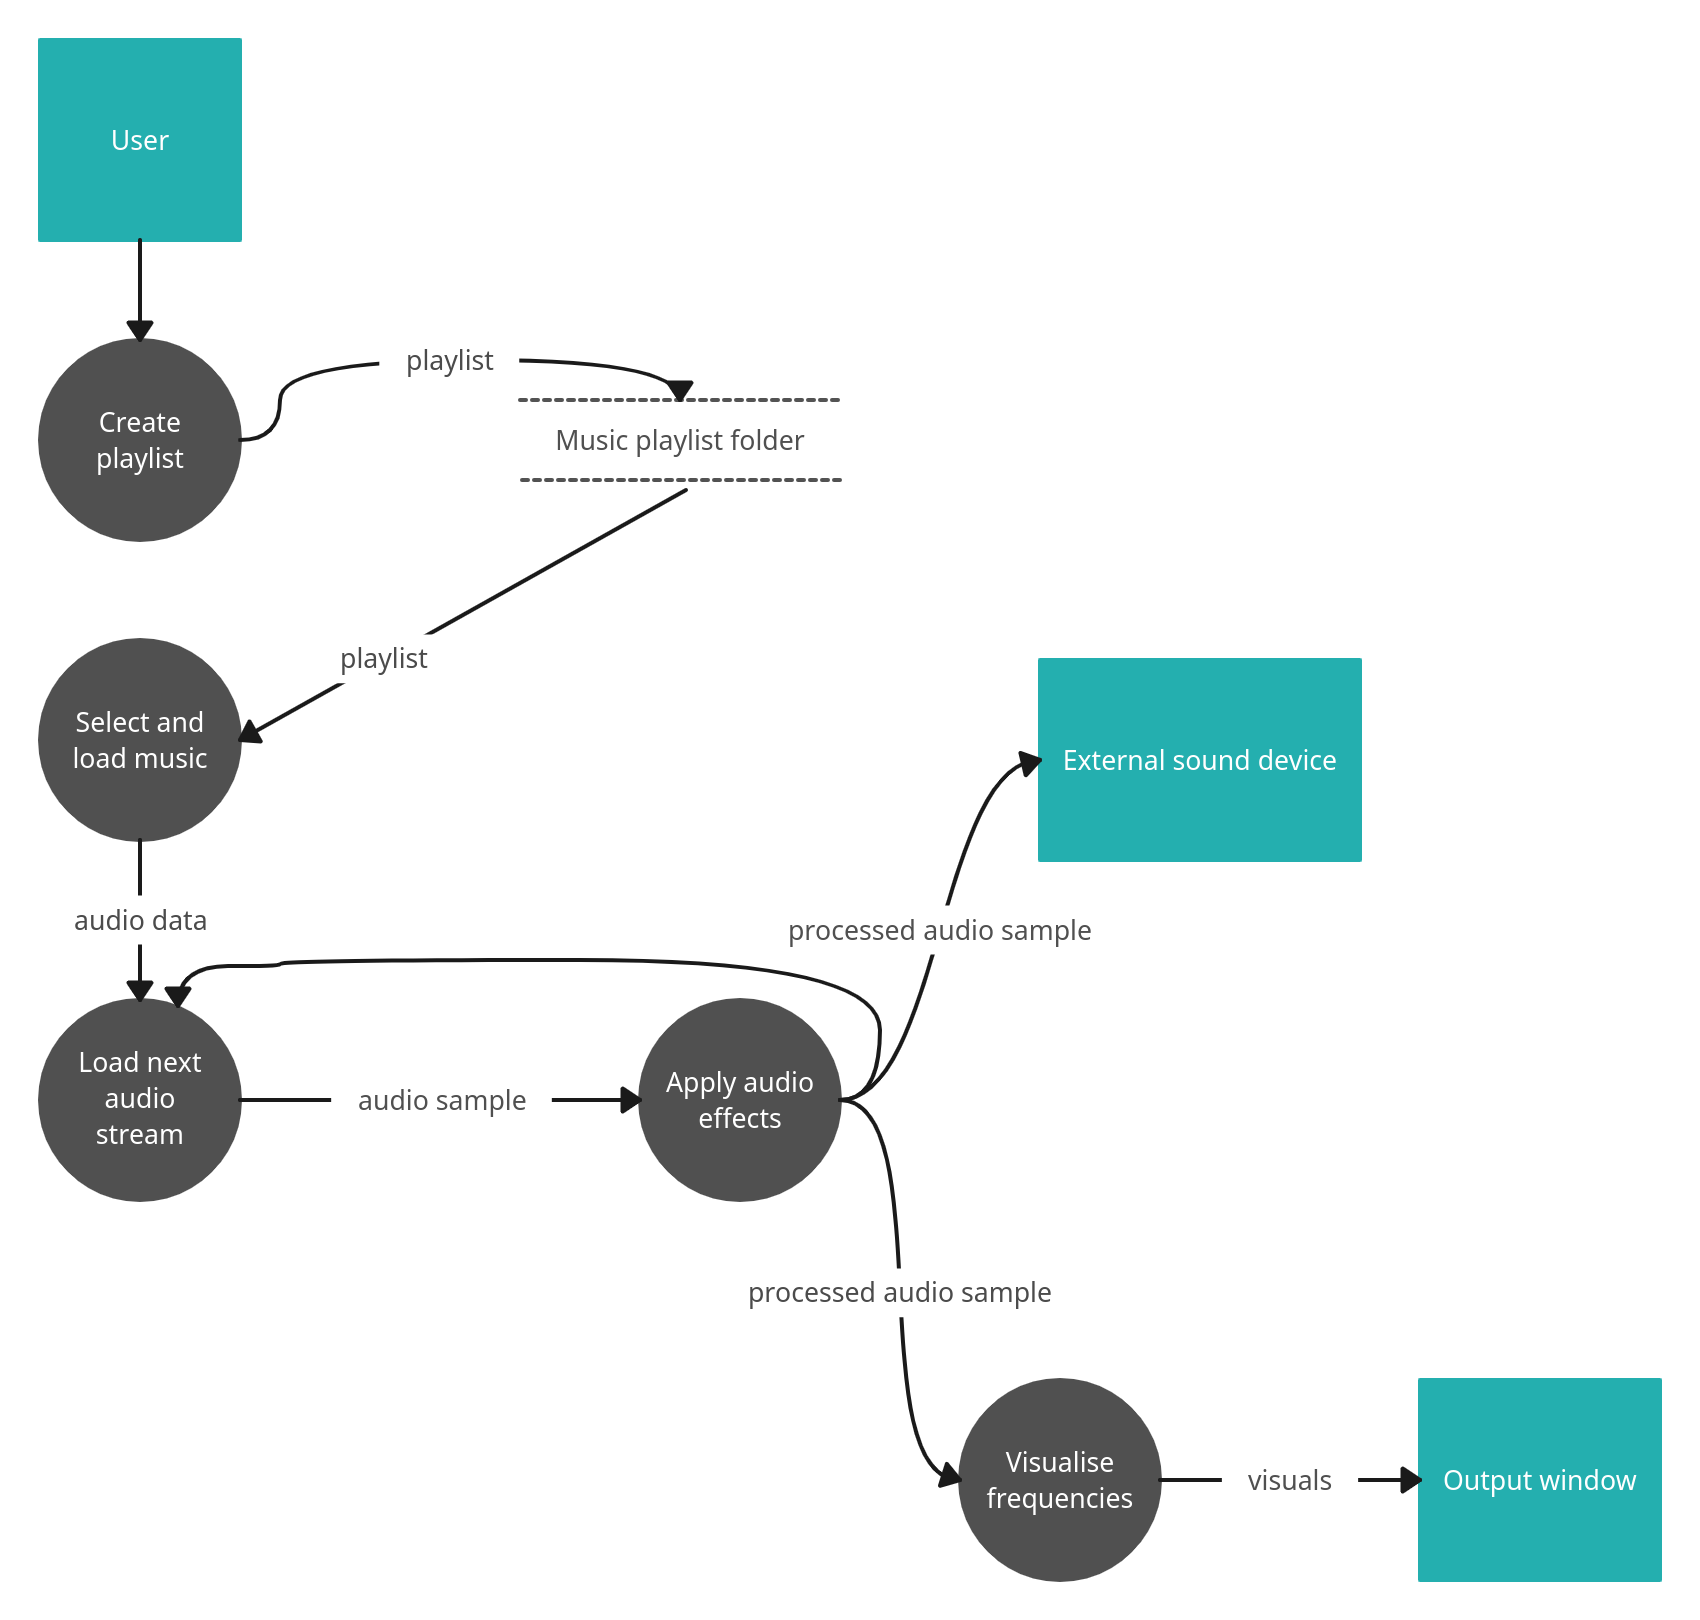
\includegraphics[width=13cm]{./DFD.png}
	\caption{The data flow diagram (DFD)}
\end{figure}

\pagebreak
\subsection{Analysis of Similar Software Products}
Every consideration must be given to the existence of other software products which may implement, either partially or fully, the features of the program yet to be implemented, in order to highlight the niche in which this project falls.

\paragraph{}
There exists two broad categories of software which provides features similar to this project:
\begin{itemize}
	\item Real-time music players - the majority of music listeners listen to music in real-time using streaming services such as Spotify or Apple Music, which can provide certain features to adjust songs in frequency-space (albeit crudely)

	\item Audio editors - for those who wish to radically alter audio (e.g. to create a remix), software such as Audacity provides many effects and processing opportunities. These are, however, "offline" in the sense that such software is not real-time.
\end{itemize}

\subsubsection{Streaming Services}
Currently within the market the two most popular music streaming products are Apple Music, with 88 million customers in 2022, and Spotify, which over 500 million. These allow users to listen to music on-demand, with both providing an "equaliser" feature that allows the user to modify the relative volume of frequencies within a song in real-time. In other words, with both these products one can, for example, alter the bass of a song, which mirrors very closely one of the main aims of this project.

\begin{figure}[H]
	\caption{The Spotify equaliser}
	\begin{center}
		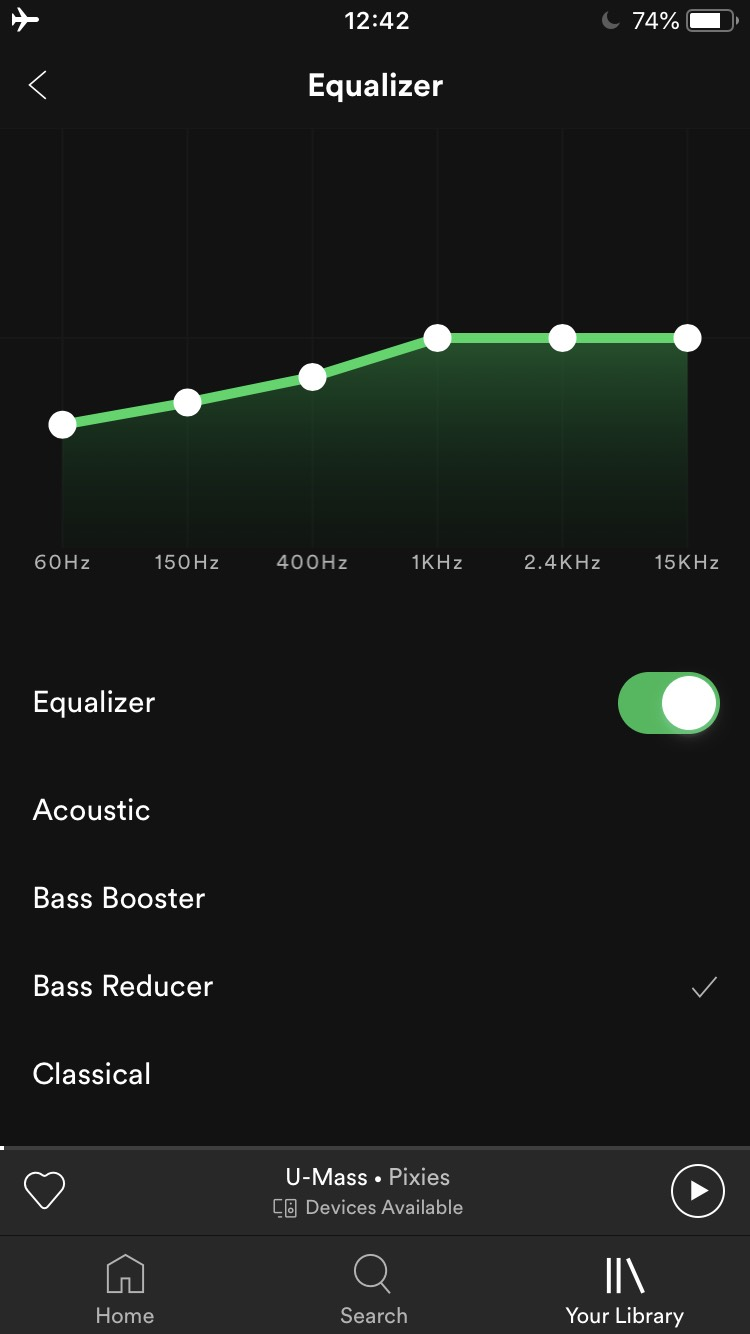
\includegraphics[width=5cm]{./spotify equaliser.jpg}
	\end{center}
\end{figure}

\begin{figure}[H]
	\caption{The Apple equaliser}
	\begin{center}
		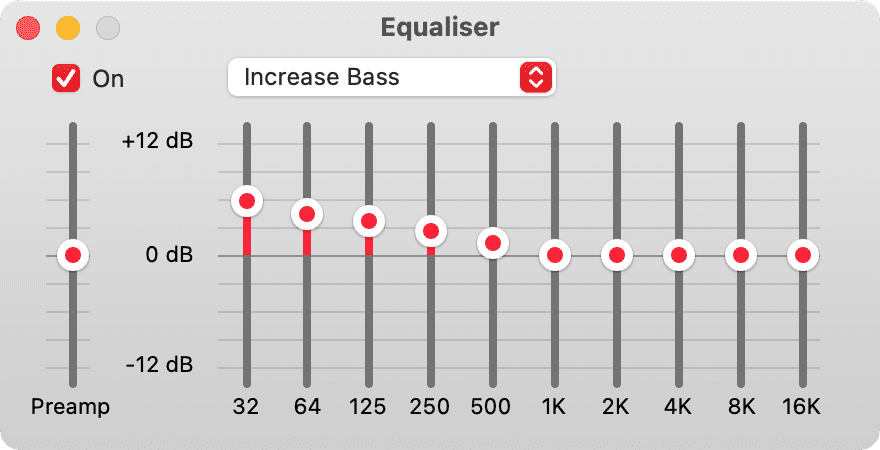
\includegraphics[width=10cm]{./apple equaliser.png}
	\end{center}
\end{figure}

As can be seen above, there are a number of similarities with the aims of this project:
\begin{itemize}
	\item The user can easily drag various points  to modify the relative volumes of a number of "frequency groups". For example, one could drag the left-most dot to its maximum height in both to boost frequencies under either 60 or 30 Hz.
	\item Ready-made "presets" can be chosen at will to assist those who may be unfamiliar with the settings presented or want to achieve a particular, pre-made effect.
	\item In Apple Music, the overall volume of the music can be adjusted.
\end{itemize}

\paragraph{}
However, there are also a few notable areas in which the two products above fall short of the features being implemented in this project, and hence fail to satisfy the needs of the users outlined in section 1.1.
\begin{itemize}
	\item In neither case does the user have exact control over the precise frequencies being modified.  If, for example, one had identified a particularly intriguing instrument playing from 500 Hz - 700 Hz, it would be impossible to isolate that frequency and boost it.
	\item There is no option to apply other audio effects such as an echo or noise. As such there are very few ways one can actually modify the audio, so creating a full "remix", that feels distinct from the original, is impossible.
\end{itemize}

\paragraph{}
Thus whilst on a surface-level, the presence of "audio equalisers" in both software products may appear to conflict with the aims of this project, especially as they perform their processing in real-time, closer inspection reveals that they offer only extremely limited options, without the ability to customise which precise frequencies are adjusted or indeed apply any other audio effects.

\subsubsection{Audio Editing Software}
On the other hand, there exists many programs which allow a user to modify audio using a great range of effects and filters. As the aim of this project is to lower the barrier of entry to creating song "remixes", it is to be free, and as such it is most worthwhile only considering other free audio editing software.

\paragraph{}
The most popular free audio editing application is Audacity, an open-source project that supports an extremely large number of effects. Additionally, it supports viewing a spectrogram of the audio being played (which visualises the audio in frequency-space just like this project aims to do), although the feature is somewhat hidden away.

\begin{figure}[H]
	\caption{Audacity when configured to display a spectrogram of the audio, seen as two multi-coloured strips (one for each channel)}
	\begin{center}
		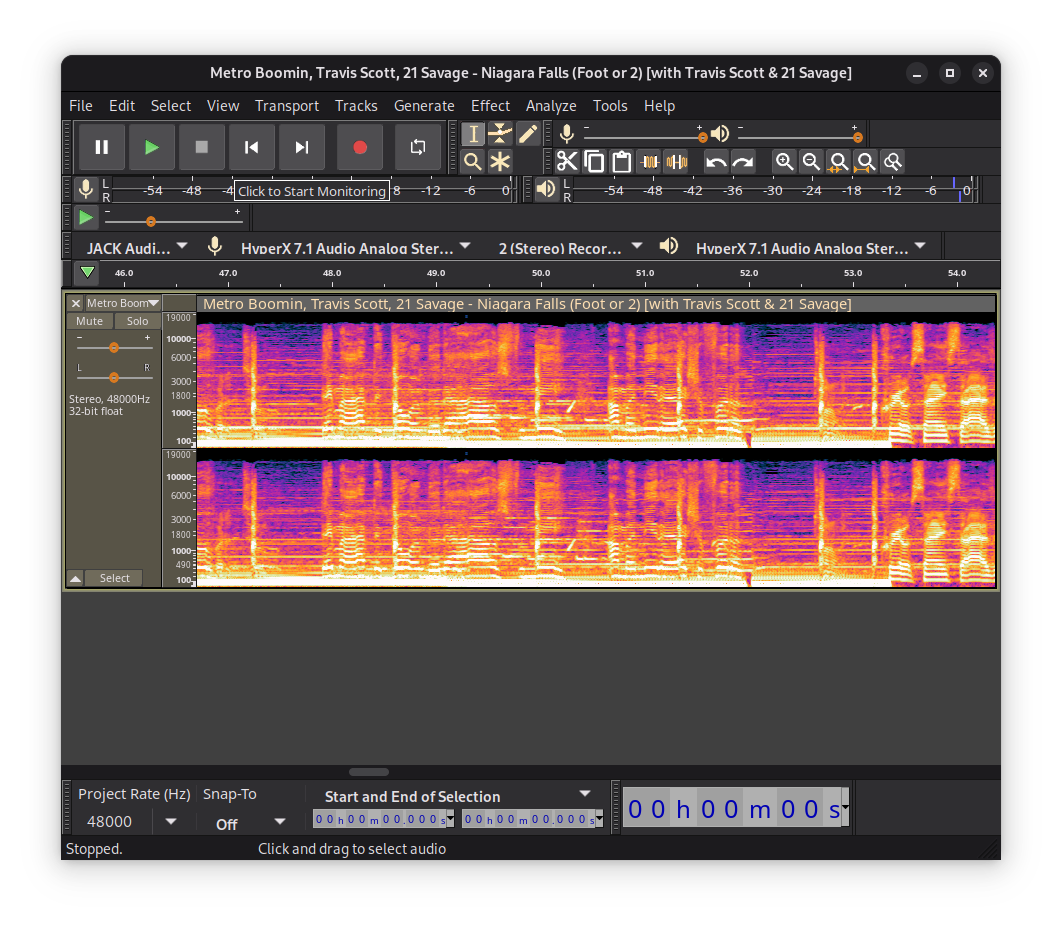
\includegraphics[width=15cm]{./audacity spectogram.png}
	\end{center}
\end{figure}

\begin{figure}[H]
	\caption{Audacity's "effects menu", offering a number of categories which themselves all contain numerous effects}
	\begin{center}
		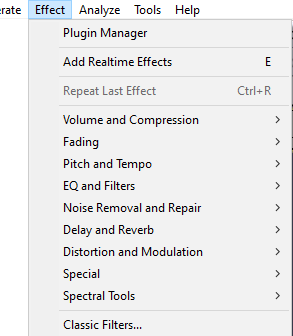
\includegraphics[width=5cm]{./audacity effects menu.png}
	\end{center}
\end{figure}

\begin{figure}[H]
	\caption{Audacity offering a menu to configure the application of a computationally-intensive, though highly accurate, reverb effect}
	\begin{center}
		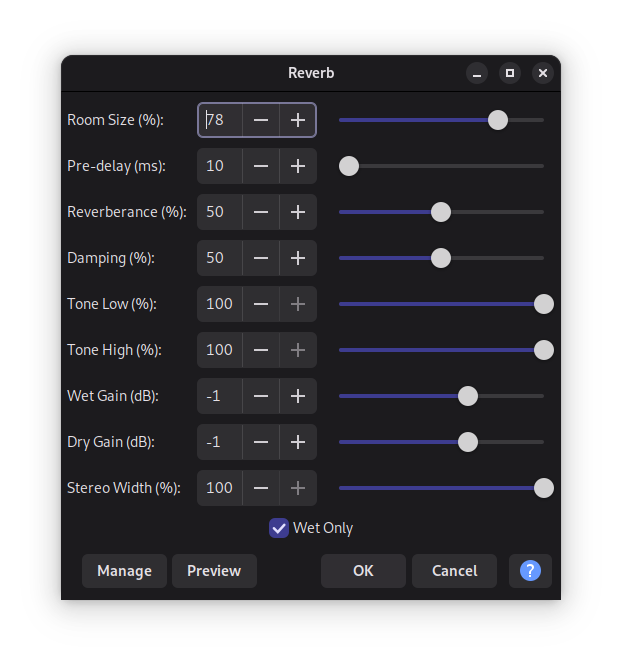
\includegraphics[width=9cm]{./audacity effects.png}
	\end{center}
\end{figure}

\paragraph{}
As can be seen above, Audacity thus presents a number of strengths which could be seen to risk overshadowing this project:
\begin{itemize}
	\item A great number of effects are supported, far greater than this project's scope could hope to provide
	\item The effects are all highly physically accurate, with extreme levels of customisation
\end{itemize}

However, its weaknesses should also be stressed:
\begin{itemize}
	\item The user interface is daunting for new users, raising the barrier of entry. For example, the process of displaying a spectrogram is not at all obvious and is hidden away.
	\item The sheer number of parameters for controlling effects is likely very daunting for people that just want a "quick remix".
	\item There are no ready-made "presets" for those too confused to immediately start applying effects themselves, or for those quickly looking for a specific modification.
	\item One cannot apply any effects in real-time, and often the effects are so computationally expensive that one must wait multiple seconds before hearing the result, even on powerful hardware.
	\item It is impossible to create a "music playlist" to listen to multiple songs in quick succession.
\end{itemize}

Hence it can be seen that whilst Audacity, and other audio editing software, provides many mechanisms for manipulating audio, it cannot be done in real-time, and often powerful hardware is required. They are also completely unsuitable as real-time music players, as they cannot play "playlists". Additionally, the sheer range of editing options would likely prove daunting to even the most experienced user, and so when one considers the high barrier of entry, the failure to be real-time, and the lack of "playlist" functionality, it is clear that audio editing programs such as Audacity do not conflict with the aims of this project.

\subsubsection{Summary of Similar Software Products}
\begin{figure}[H]
	\caption{S.W.O.T diagram for streaming services}
	\begin{center}
		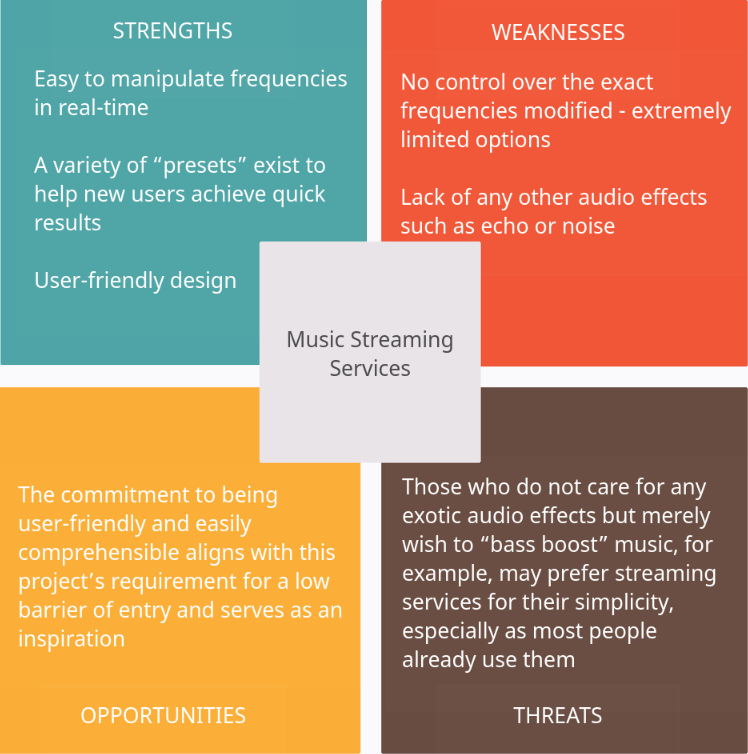
\includegraphics[width=10cm]{./SWOT streaming.png}
	\end{center}
\end{figure}
\begin{figure}[H]
	\caption{S.W.O.T diagram for audio editing prograrms}
	\begin{center}
		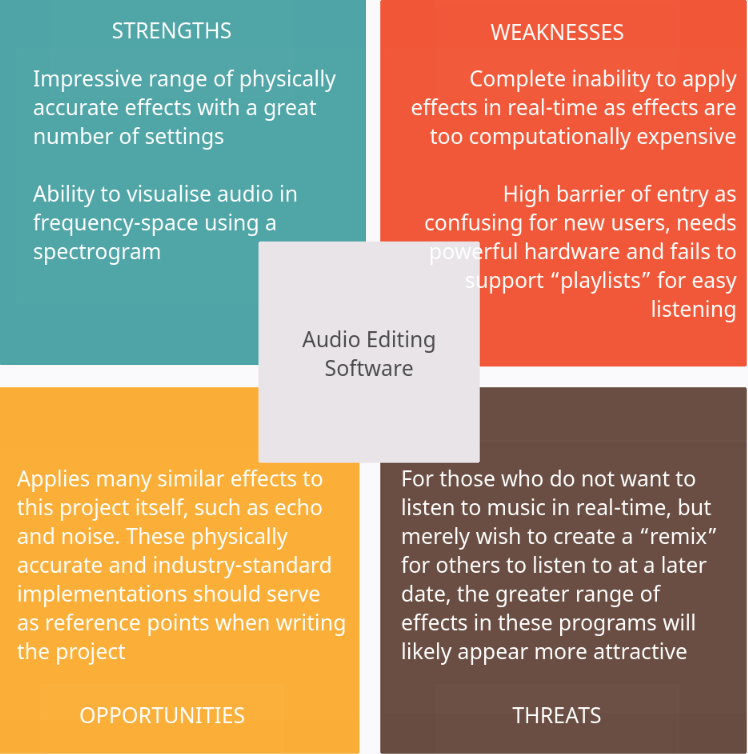
\includegraphics[width=10cm]{./SWOT audacity.png}
	\end{center}
\end{figure}

\pagebreak
\subsection{Final objectives}
\begin{enumerate}
	\item  The user must be able to load a collection of audio files known as a "playlist" and then play the audio files contained within, organised alphabetically, as is the custom in audio-listening applications.
	\item  The user must be able to visualise the current audio being played in the frequency domain (i.e. visualise the frequencies)
	\item The user must be able to modify the audio's frequency domain (i.e. selectively modify frequencies such as by reducing the bass)
	\item The user must be able to apply additional "audio effects" to further enhance the music: echo, volume adjustment and noise
	\item The user must be able to configure these "audio effects" individually, yet also apply pre-made "presets" to quickly reach a desired effect
	\item  The system must run in real-time on an average school computer
	\item The user must be able to alter the speed at which audio is played
\end{enumerate}
	\section { Design }

\subsection{Multithreading}
In order to maximise ease-of use, the software should have a graphical user environment (GUI) so that the current audio being played can be easily visualised (in-line with objective 2). The program will use a multithreaded model, with a separate "audio thread" and "GUI thread", allowing the two to run concurrently without blocking each other's processing.

\begin{figure}[h]
	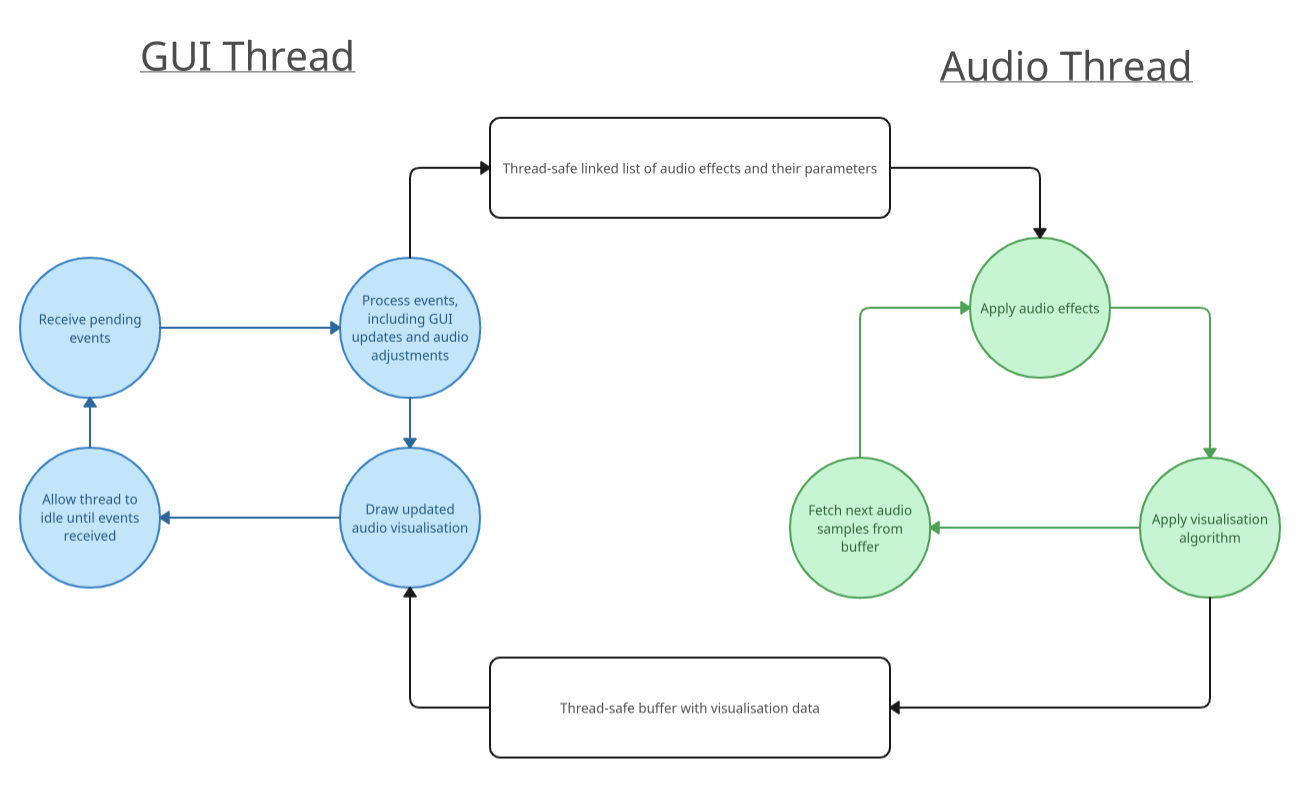
\includegraphics[width=17cm]{./threading.png}
	\caption{Inter-thread diagram - see below for justification for thread-safe data structures}
\end{figure}

\paragraph{}
Typically, GUI programs are written using an event-based paradigm that minimises CPU idle-time. The consequence of this is that, for most of the time, the GUI thread is suspended, awoken only when events from the user (such as mouse clicks or resizing the window) "wake it up". This is desirable in order to minimise system resources used, as more CPU-time will be available for the audio processing requirements, helping to reach the real-time requirements of objective 6. However, this presents a unique challenge. With a single-threaded model:
\begin{itemize}
	\item If the event-based model is followed, the GUI thread is only active when there are pending GUI events to be processed, meaning audio processing can only occur sporadically (resulting in "non-constant" audio)
	\item If instead the GUI thread is constantly active processing audio it will never reach a point where it can process pending events, meaning the program will hang and refuse to process inputs.
\end{itemize}

Hence it is desirable to split the program into two distinct threads. The audio thread can play the audio and perform all necessary processing tasks, whilst the GUI thread can relay input parameters and commands to the audio thread (such as "switch song", "apply effect", etc.).

\paragraph{}
To avoid race conditions\footnote{
	 Race conditions occur when one thread tries to read data whilst the other writes to it. If, for example, the GUI thread removed an audio effect from the audio effect list (see above) and freed it from memory whilst the audio thread was applying that same effect, the audio thread would suddenly be reading from invalid memory, likely resulting in a crash or undefined behaviour.
}, the data that is read by both threads should be thread-safe - only one thread should be able to access the data at a time. This can be achieved by using mutexes\footnote{
	A mutex is an object that prevents multiple threads from accessing data at the same time. It can be thought of as a lock, which can only be unlocked for one thread at a time. They are preferable to spinlocks as they do not require the CPU to waste cycles waiting for the data to be "unlocked", as instead the thread can suspend itself until the mutex becomes available.
}.

\subsubsection{Audio Effects Data Structure}
\paragraph{Picking a data structure} The user will likely want to adjust the order of audio effects at will, and as the same time, it must be very fast to insert and  remove audio effects so as to minimise the time spent not processing audio (even a very short pause may result in "crackles" on weaker hardware). To solve this problem, the audio effects can be stored in a linked list, as unlike std::vectors (dynamic C++ arrays) they prove fast insertion, deletion and swapping irrespective of the number of elements stored.

\paragraph{Making it thread-safe}
To satisfy the requirements of multithreading (see above), I will write my own custom "atomic linked list", backed by a mutex\footnote{
	See above footnote on mutexes
}, which will function just like a normal linked list but maintain thread-safety in all its operations.


\pagebreak

\subsection{Audio Data and Playback}

\subsubsection{Audio Data}
The program will have to load a variety of  user-supplied data in order to operate:
\begin{itemize}
	\item As described in objective 1, the user must be able to load a collection of audio files known as  a "playlist", which will contain the paths of one or more audio files on the system.
	\item Each audio file will consist of a number of audio samples, which will need to be loaded into memory when needed, then freed when not in use.
	\item Audio files also contain other crucial information, such as the audio frequency (e.g. 44,000 Hz), the number of channels (usually mono (1) or stereo (2)), and the number of samples (the "length").
	\item Thus to keep track of the audio files loaded into memory, each audio file will need to store its raw audio samples, its frequency, the number of channels, and the number of samples.
\end{itemize}

\subsubsection{ Audio Data UML }
\begin{figure}[H]
	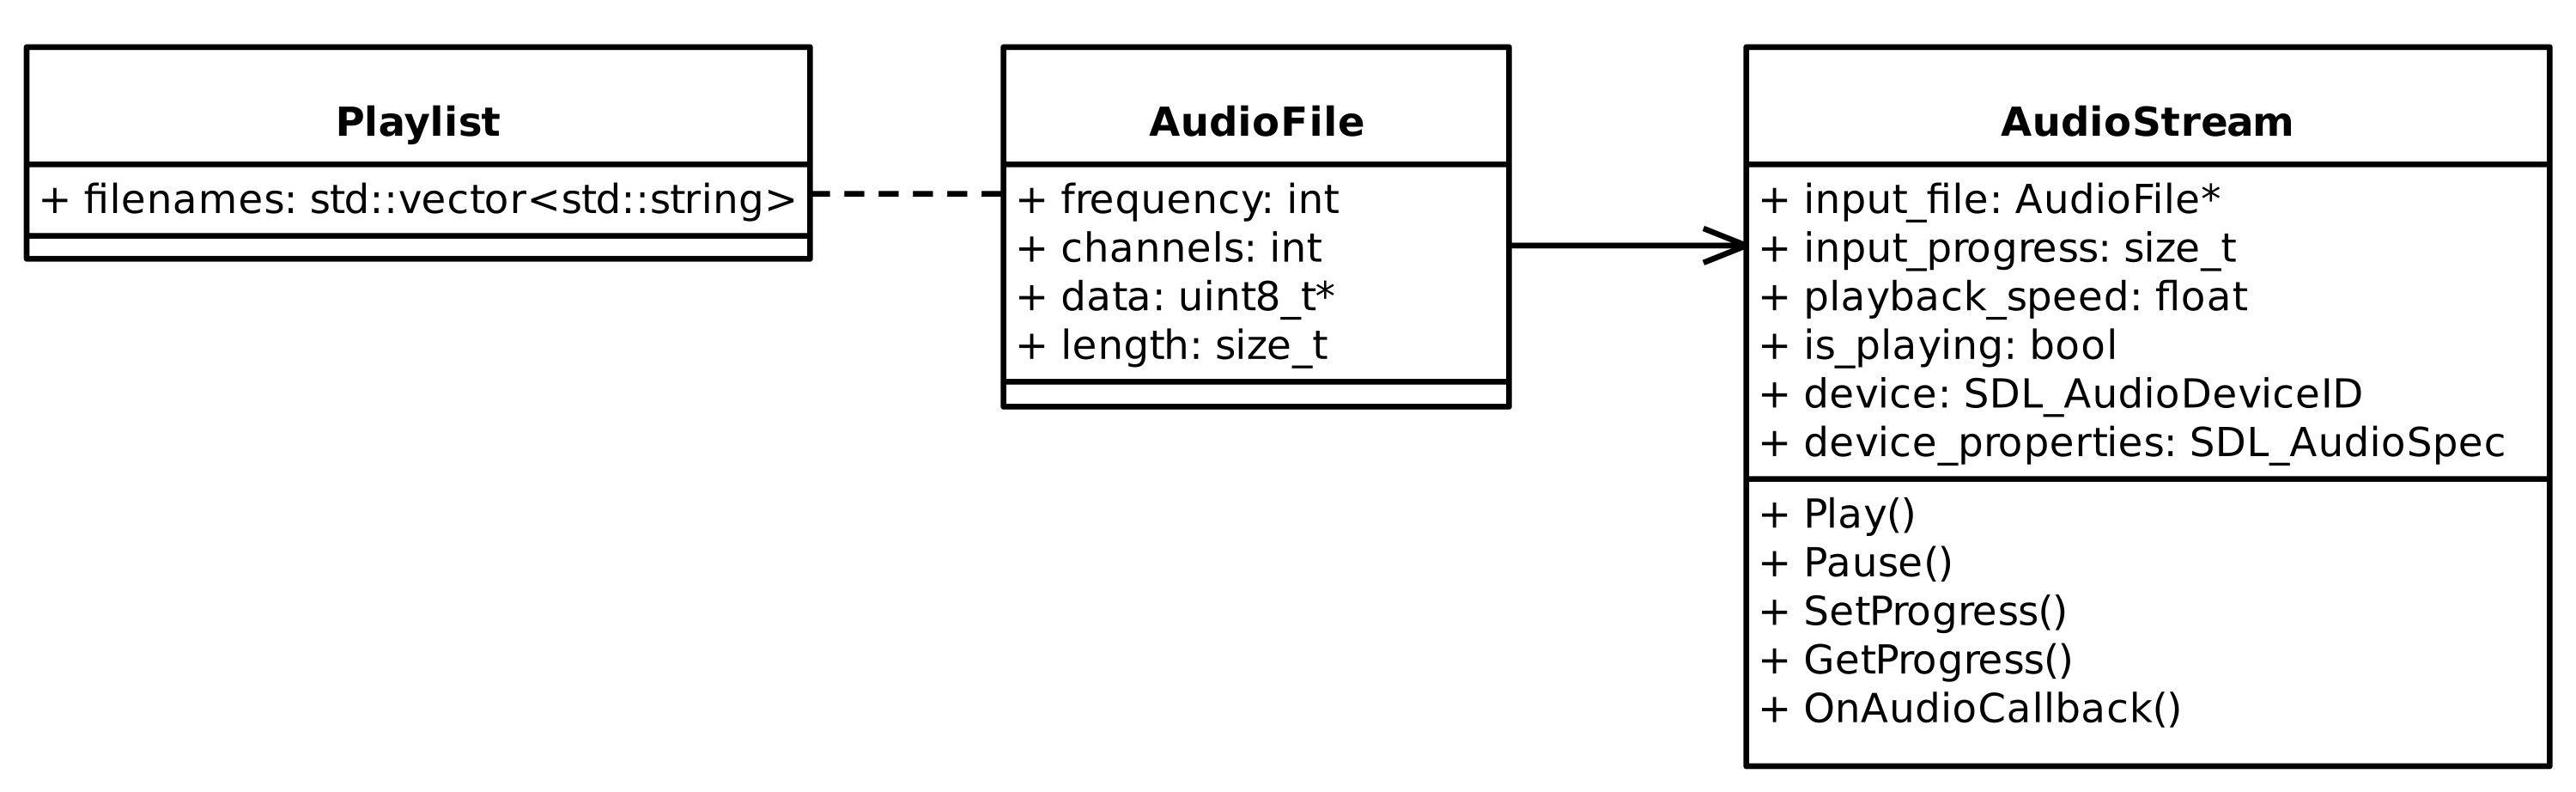
\includegraphics[width=14cm]{./audio io uml.png}
	\caption{UML for Audio Data and IO - separate getter and setter exists for AudioStream progress as the caller will express progress as percentage (e.g. 50\% played) so that it is independent of file size. The playlist contains the filenames of all audio files on disk, and an AudioFile instance is created, when needed, by loading the audio file from disk using this filename. }
\end{figure}

\subsubsection{The Need for Streaming}
It may be tempting to load and unload all audio data in a hierarchal  fashion as such:
\begin{enumerate}
	\item An attempt is made in the code to load a playlist.
	\item To do this, the playlist will be read from disk and all the audio file paths contained within will be loaded into memory.
	\item Each audio file path will be verified to check it is valid exists on the system.
	\item If the playlist is valid, each audio file will then be loaded using the paths provided.
	\item Thus the loading of a playlist will involve loading all audio files referenced within.
	\item At the end of the program, when the playlist is no longer needed, all the playlist's audio files will be freed from memory, followed by the playlist itself.
\end{enumerate}

However, this is not a practical approach due to memory usage constraints. If a user attempted to load a playlist consisting of 200 songs, each 5 MB each, this would consume roughly 1000 MB of memory for the entire duration of the program, even though only 1 audio file can be played at once (and hence only one needs to be in memory at any one time). This conflicts with objective 6 ("the system must run in real-time on an average school computer") as many computers may not have large amounts of free memory, particularly if other programs are running, which may lead to an out-of-memory crash.

\paragraph{}
Instead, I have decided to "stream" audio files as they are played, so that only the audio file currently needed is resident in memory. This can be modelled as followed:
\begin{enumerate}
	\item An attempt is made in the code to load a playlist.
	\item To do this, the playlist will be read from disk and all the audio file paths contained within will be loaded into memory.
	\item Each audio file path will be verified to check it is valid exists on the system. If the playlist is valid, the execution of the program will continue.
	\item Each time the next audio file is to be played from the playlist, the program will dynamically load it from disk (using the path from the playlist) and store it in memory.
	\item When the next audio file is chosen, it is loaded as described above. Crucially however, the previous audio file is first unloaded from memory, as it is no longer needed.
	\item At the end of the program, the currently playing audio file and playlist are both freed.
\end{enumerate}

\paragraph{}
In this way, the issue of large playlists resulting in extremely large memory consumption will be avoided, as only one audio file will be loaded at once.

\subsubsection{Audio Playback}
The playback of audio itself presents many challenges. In order to make the code as modular and decoupled as possible, I will abstract away the low-level creation of audio devices, pausing, un-pausing, etc. into an "AudioStream" class. One will simply create an "AudioStream", supply it with data, and the class will manage the various complexities of multithreading and feed the audio buffer with data at the appropriate times.

\paragraph{}
In order to maximise portability of the code,  and hence make it as cross-platform as possible in order to maximise the program's audience, I have decided to use a library called "SDL2" to handle audio playback, as it abstracts away the native APIs one would have to otherwise use. In this way, separate audio code does not have to be written for Windows, Linux, etc.

\paragraph{}
The code that plays audio on the system will run on a separate thread (see multithreading section). This audio thread is invoked at regular intervals by the operating system by way of a "callback" function. When this happens, it is the program's responsibility to supply the operating system with the next buffer of audio. This is summarised below:

\begin{enumerate}
	\item An "AudioStream" is created and supplied with the raw audio samples from the audio file, as well as pointers to the atomic linked list of audio effects and to the visualisation data buffer.
	\item The AudioStream uses SDL2 to invoke audio playback at regular intervals on a separate thread (the "audio thread") using a callback
	\item Every time the callback is called, the AudioStream will fetch the next section of upcoming audio that it has been supplied with.
	\item Each audio effect will then be applied (using the audio effects atomic linked list).
	\item The audio visualisation module will then be invoked on the audio just processed, and its output written to the visualisation data buffer.
	\item Now that all work is done for the current section of audio, the processed audio will be copied to the callback's audio buffer and the audio thread will suspend itself.
	\item When the next section of audio is due, the callback will be re-invoked.
\end{enumerate}

\subsubsection { Audio Playback Flowchart }
\begin{figure}[H]
	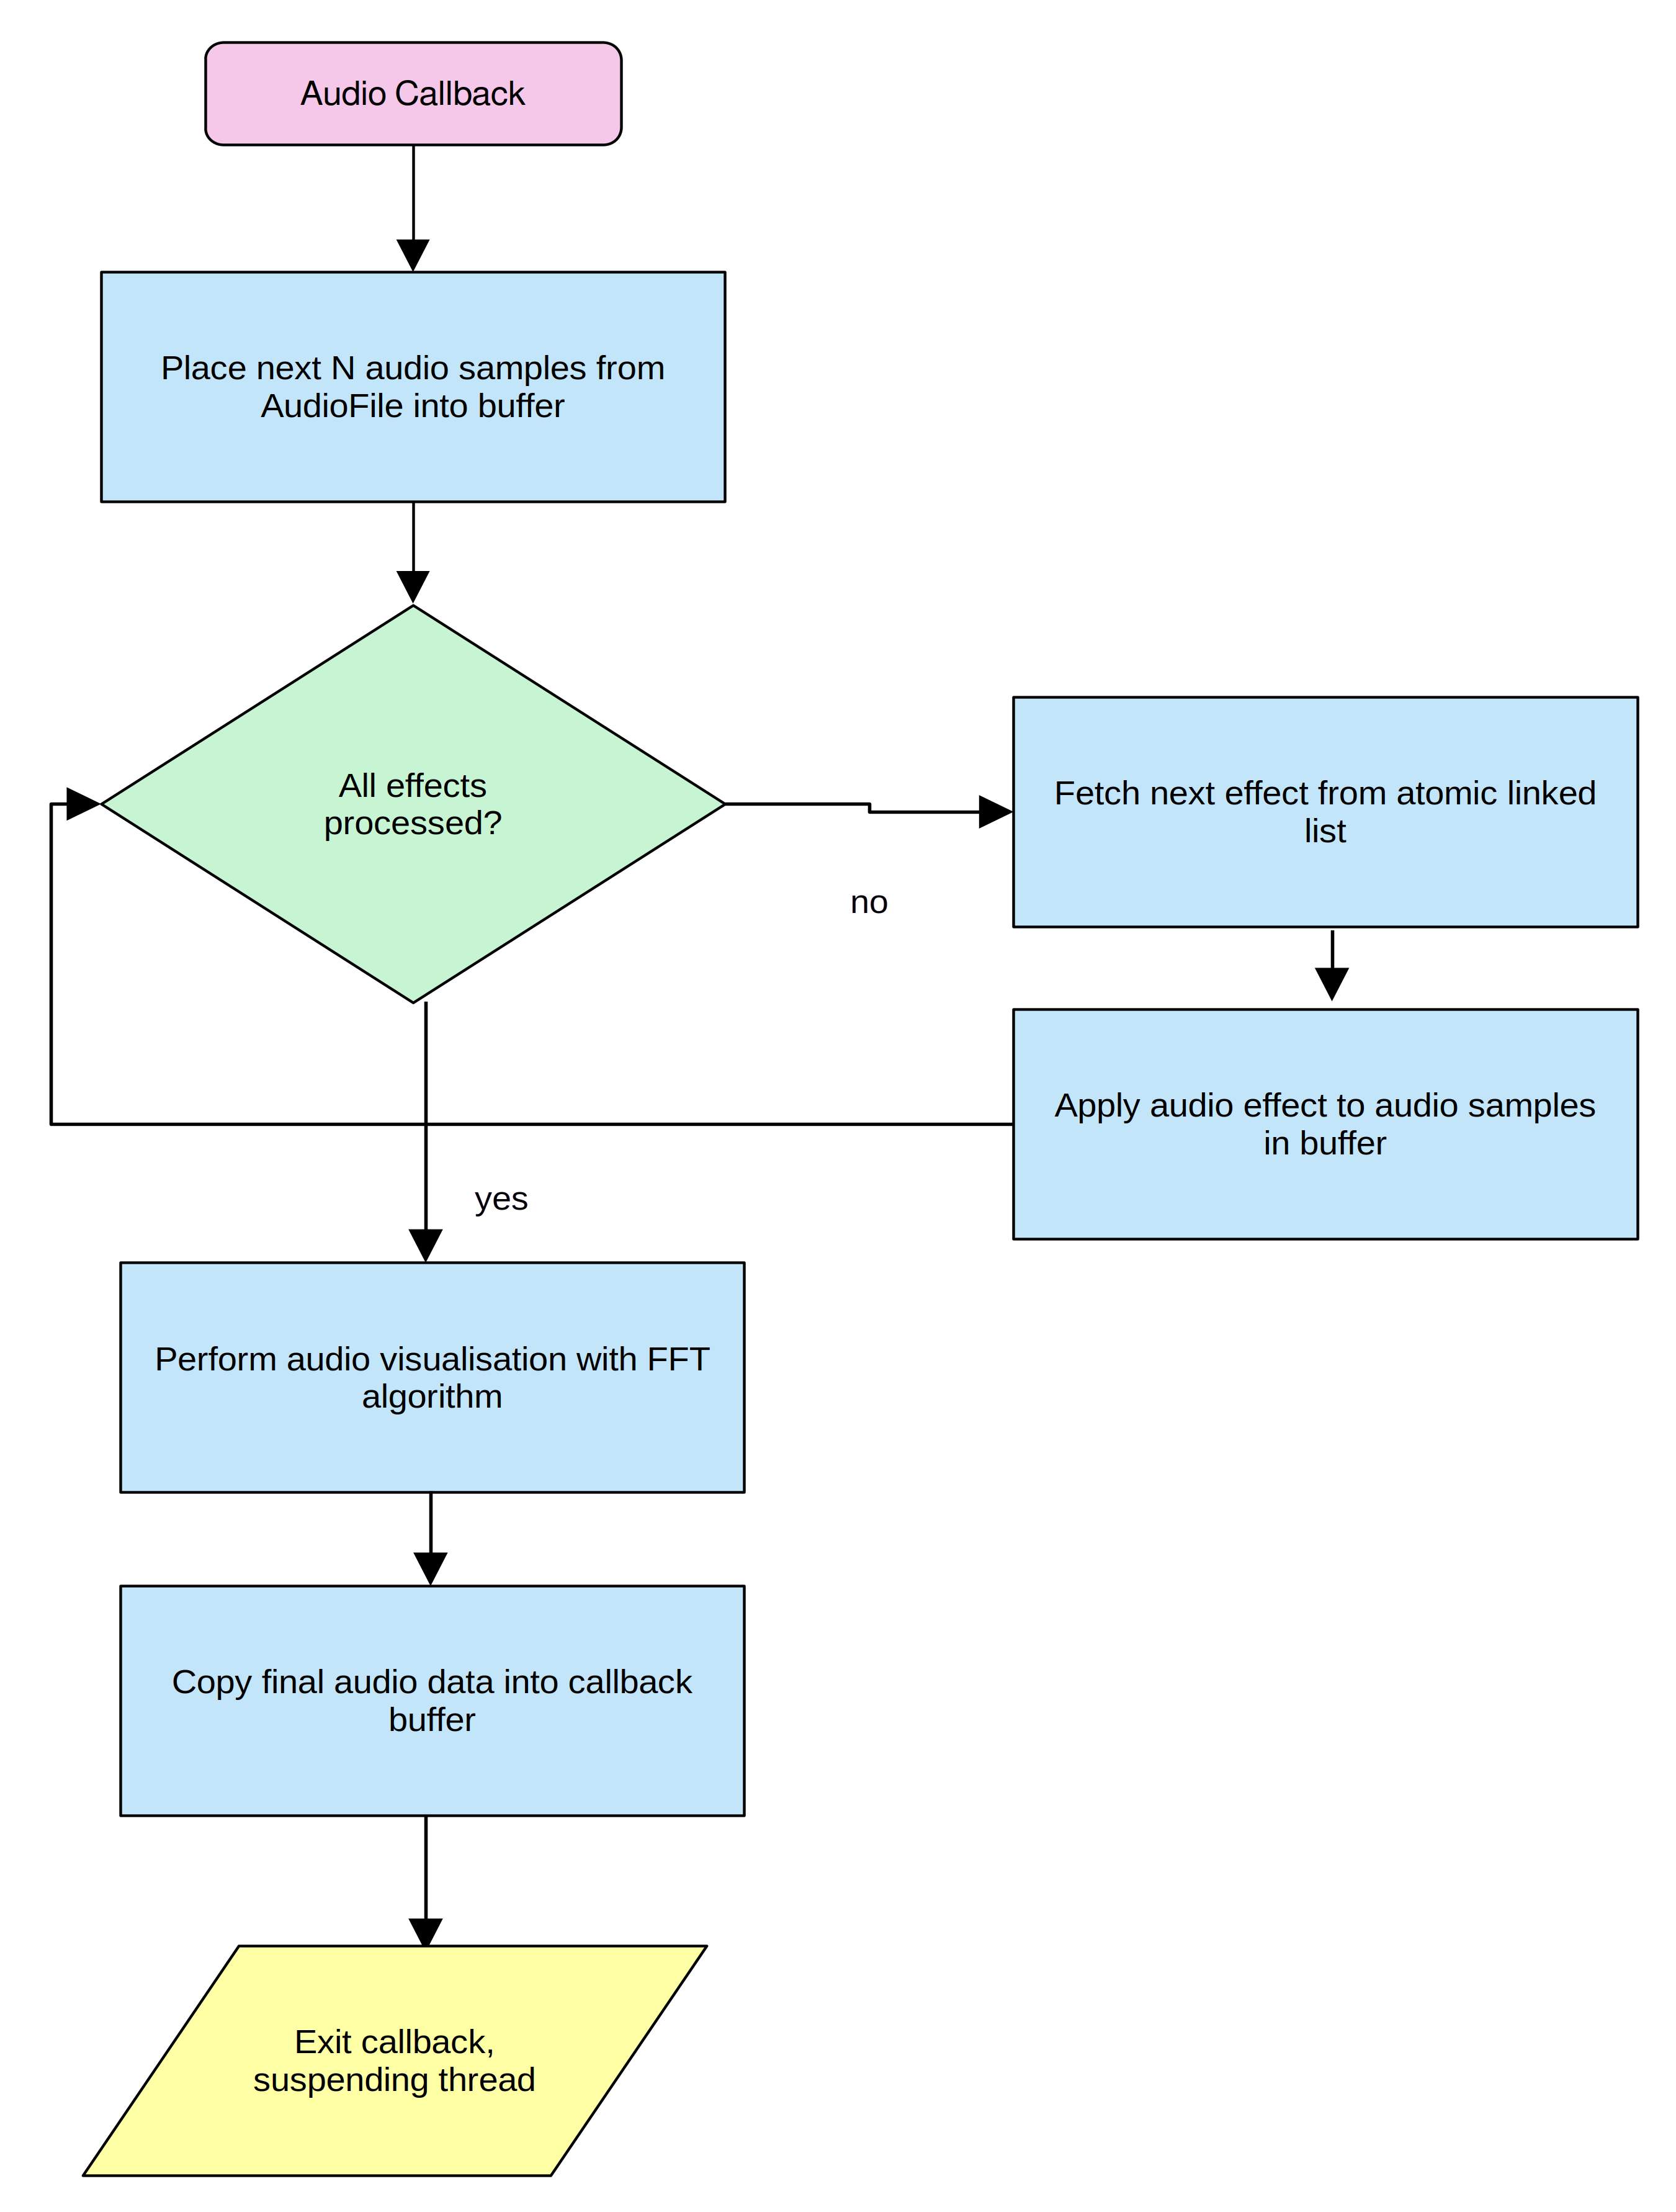
\includegraphics[width=14cm]{./audio io flowchart.png}
	\caption{Flowchart for AudioStream's SDL audio device callback}
\end{figure}

\pagebreak

\subsection{Audio Effects Architecture}
The full list of audio effects detailed in the analysis section is as follows:
\begin{itemize}
	\item Equaliser (frequency modification) - selectively modifying frequencies such as by altering the bass
	\item Echo - making audio sound like it's recorded in a large room
	\item Volume adjustment - modifying the amplitude of the audio
	\item Noise - adding subtle imperfections to the audio
\end{itemize}

\subsubsection{Unique Audio Effect Traits}
Each audio effect will need its own properties, and potentially its own mutable state (for example, the echo effect needs to "remember" the previous audio samples so it can repeat them later). Below is a summary of the requirements, properties and state of each audio effect.

{
\renewcommand{\arraystretch}{1.5}
\begin{table}[h!]
	\begin{center}
		\begin{tabularx}{1.0 \textwidth} {
				| >{\raggedright\arraybackslash}X
				| >{\raggedright\arraybackslash}X
				| >{\raggedright\arraybackslash}X
				| >{\raggedright\arraybackslash}X  |
			}
			\hline
			Effects & Requirements & Properties & State \\

			\hline
			Equaliser & Allow the user to alter the volume of a selected frequency range. Multiple equaliser effects can be applied successively to cover multiple ranges.  & Lower frequency \newline  Upper frequency \newline Multiplier  & None \\

			\hline
			Echo & Produce an echo effect where audio sounds like it's getting reflected in a large room & Fall-off (how quickly echoes fade) \newline Delay samples (how many samples must pass before a sample is echoed) & Previous audio samples buffer \\

			\hline
			Volume & Adjust the volume / amplitude of incoming audio & Volume multiplier & None \\

			\hline
			Noise & Add subtle imperfections to the audio & Intensity (the volume of the noise) & None\\

			\hline
		\end{tabularx}
	\end{center}
\end{table}
}

\pagebreak
\subsubsection{Common Audio Effect Traits}
Immediately it is obvious that all audio effects will share many common features. Each effect shall:
\begin{itemize}
	\item Take a number of audio samples as input
	\item Have a number of configurable options which need to be exposed to the GUI front-end
	\item Perform processing on all audio samples at once
	\item Output its final processed audio
\end{itemize}

\paragraph{}
Given these requirements it is wise to use an object-orientated inheritance approach where effect subclass inherits from a common parent, which provides common functionality (such as the storage and exposing of configuration options), as well as providing a common interface that other parts of the code can use. In order to abstract away the details of interacting with an audio effect, two new classes will also be needed.

\subparagraph{Packet} A packet represents a chunk of audio awaiting processing by the effect. However, some effects require knowledge of both the previous audio samples and future audio samples\footnote{
	This is because performing Fourier transforms on isolated "chunks" of audio and then
	playing them back after modification will result in a periodic "clicking" sound at the boundary between chunks due to sudden changes in sound amplitude. This is because
	of the limited resolution of a Discrete Fourier Transform. To solve this, we must take
	into account both the sound packet that comes after, and the one that comes before.
}. Thus, each packet will consist of 3 audio buffers - one for the previous, current and next buffer of audio samples. A packet will also contain the frequency of the incoming audio as this is required for the FFT maths.

\subparagraph{Property} Each audio effect has a number of configurable properties. To aid in validation, each property will have a current,  minimum and maximum value.

\paragraph{}
Both these classes will be independent of the main audio effect parent class. The audio effect parent class will merely use these classes to represent the data provided and stored by it. This is an example of {\it composition}.

\subsubsection{Properties Data Structure}
Each audio effect will have a list of properties. When drawing a properties GUI, the front-end code will want an easy and convenient way of both getting a list of all available properties, along with their respective names. In a similar fashion, when setting the values of certain properties, it will be most convenient if properties can be accessed using their names.

\paragraph{}
I will use a hash-map as my data structure for this purpose. Hash-maps can be indexed by using the name of the property (e.g. "minimum frequency" as the key), simplifying the front-end code and avoiding the need for a separate "property name" variable. In addition, they provide very fast look-up with an O(1) time, which may be important if future effects have a large number of properties to avoid wasting CPU cycles iterating through properties (e.g. if stored in a list). Whilst hash-maps are expensive when it comes to adding and removing elements, each audio effect will only have a fixed number of properties that are added once at creation so this will not be an issue.

\paragraph{Polymorphism}
Some properties will be floating point values, whilst others will be integer values. If this project is continued further, I may wish to also add boolean values as well. To accommodate this, I will use polymorphism by creating a \textit{Property} base class, then \textit{FloatingPointProperty} and \textit{IntegerProperty}  children, which will share a common interface.

\subsubsection{UML Class Diagram}
After considering all the requirements of the multiple classes required, I have constructed a class diagram. However, a slight modification has been made to the typical UML structure: \textit{properties} of audio effects appear in the lower box in each class, in order to indicate that they are not attributes {\it per se}, but rather are elements in their parent's properties hashmap.

\begin{figure}[h]
	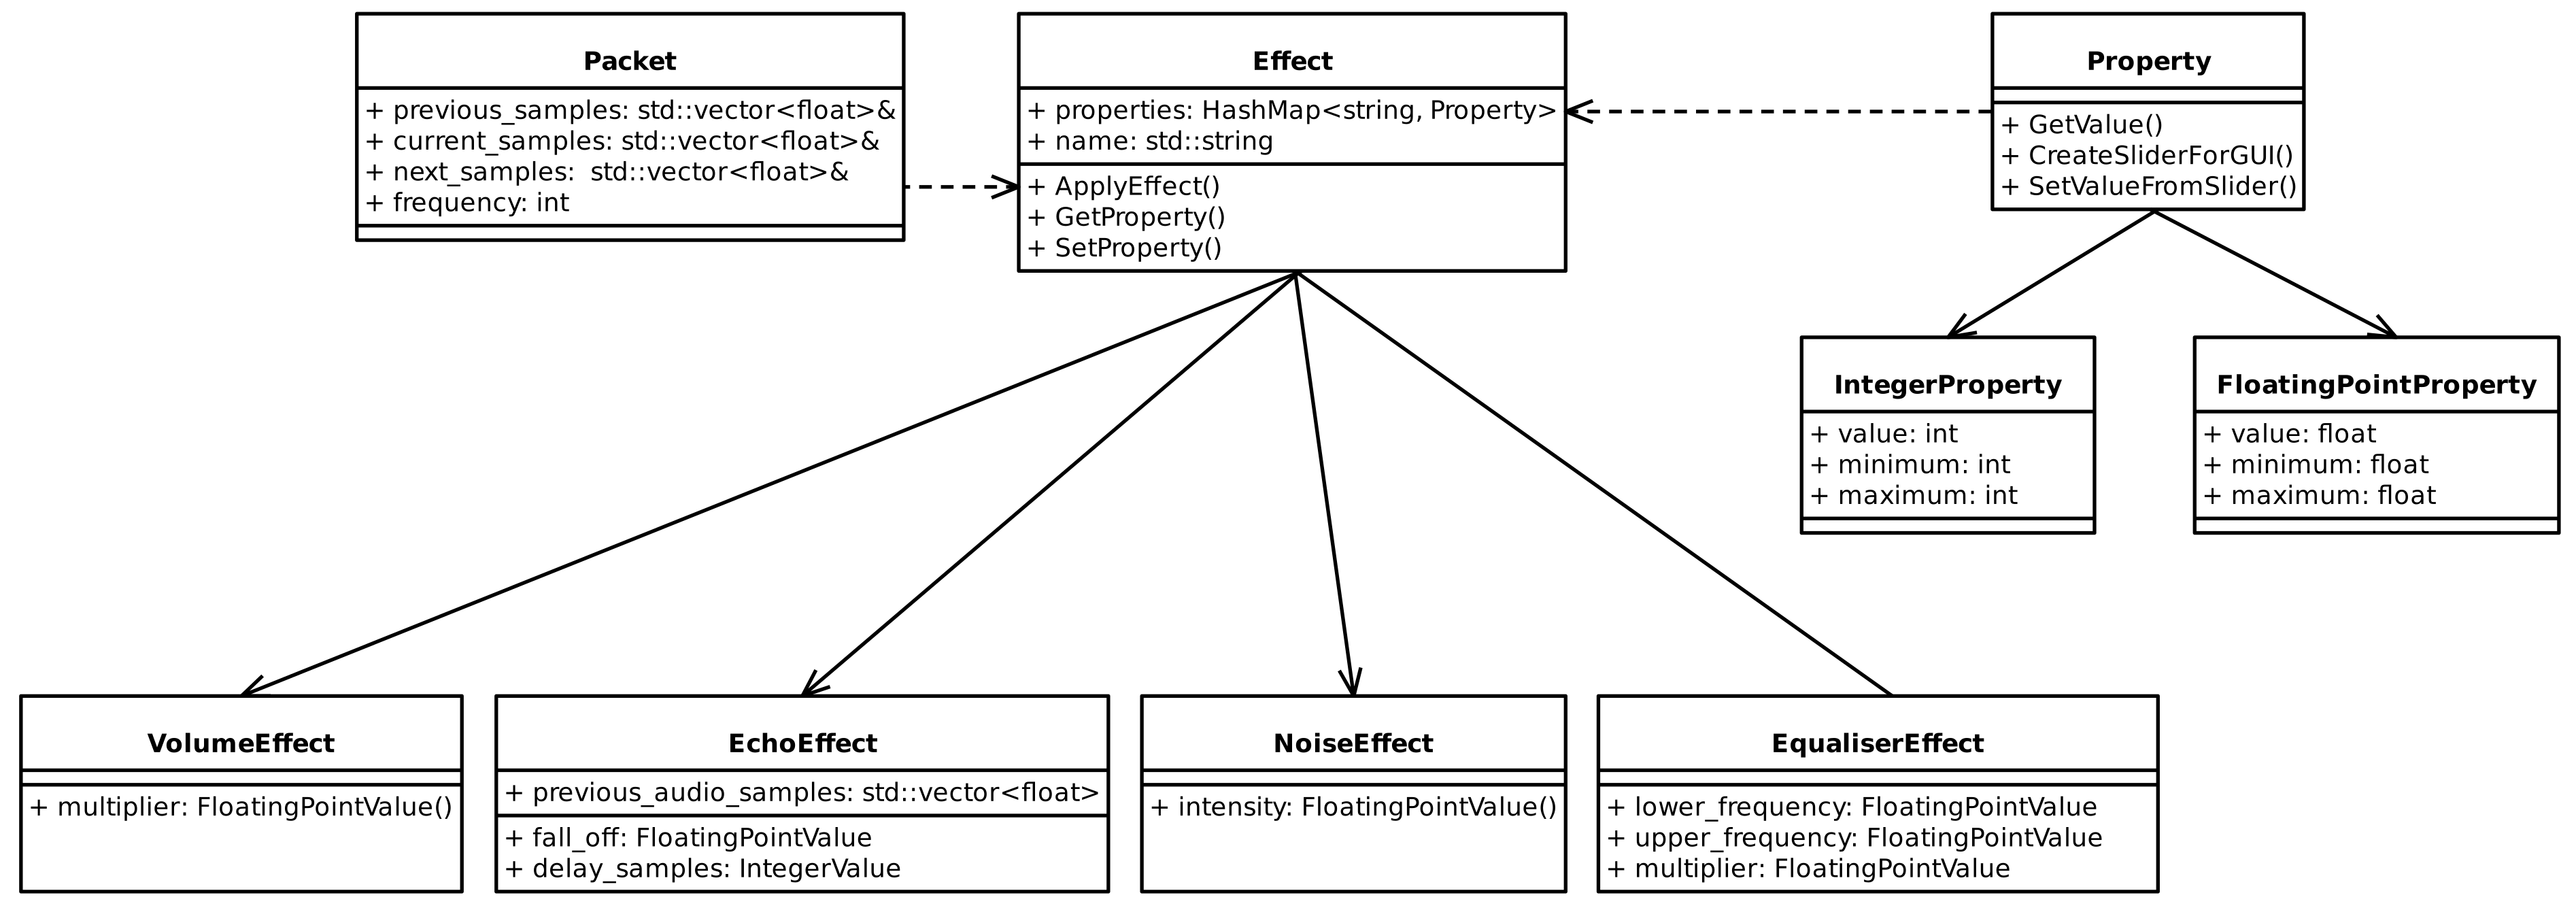
\includegraphics[width=\textwidth]{./effects class diagram new.png}
	\caption{UML class diagram containing attributes, operations and custom "properties"}
\end{figure}

\pagebreak

\subsection{High-Level Audio Effects Flowcharts}
\begin{figure}[H]
	\subsubsection{Equaliser}
	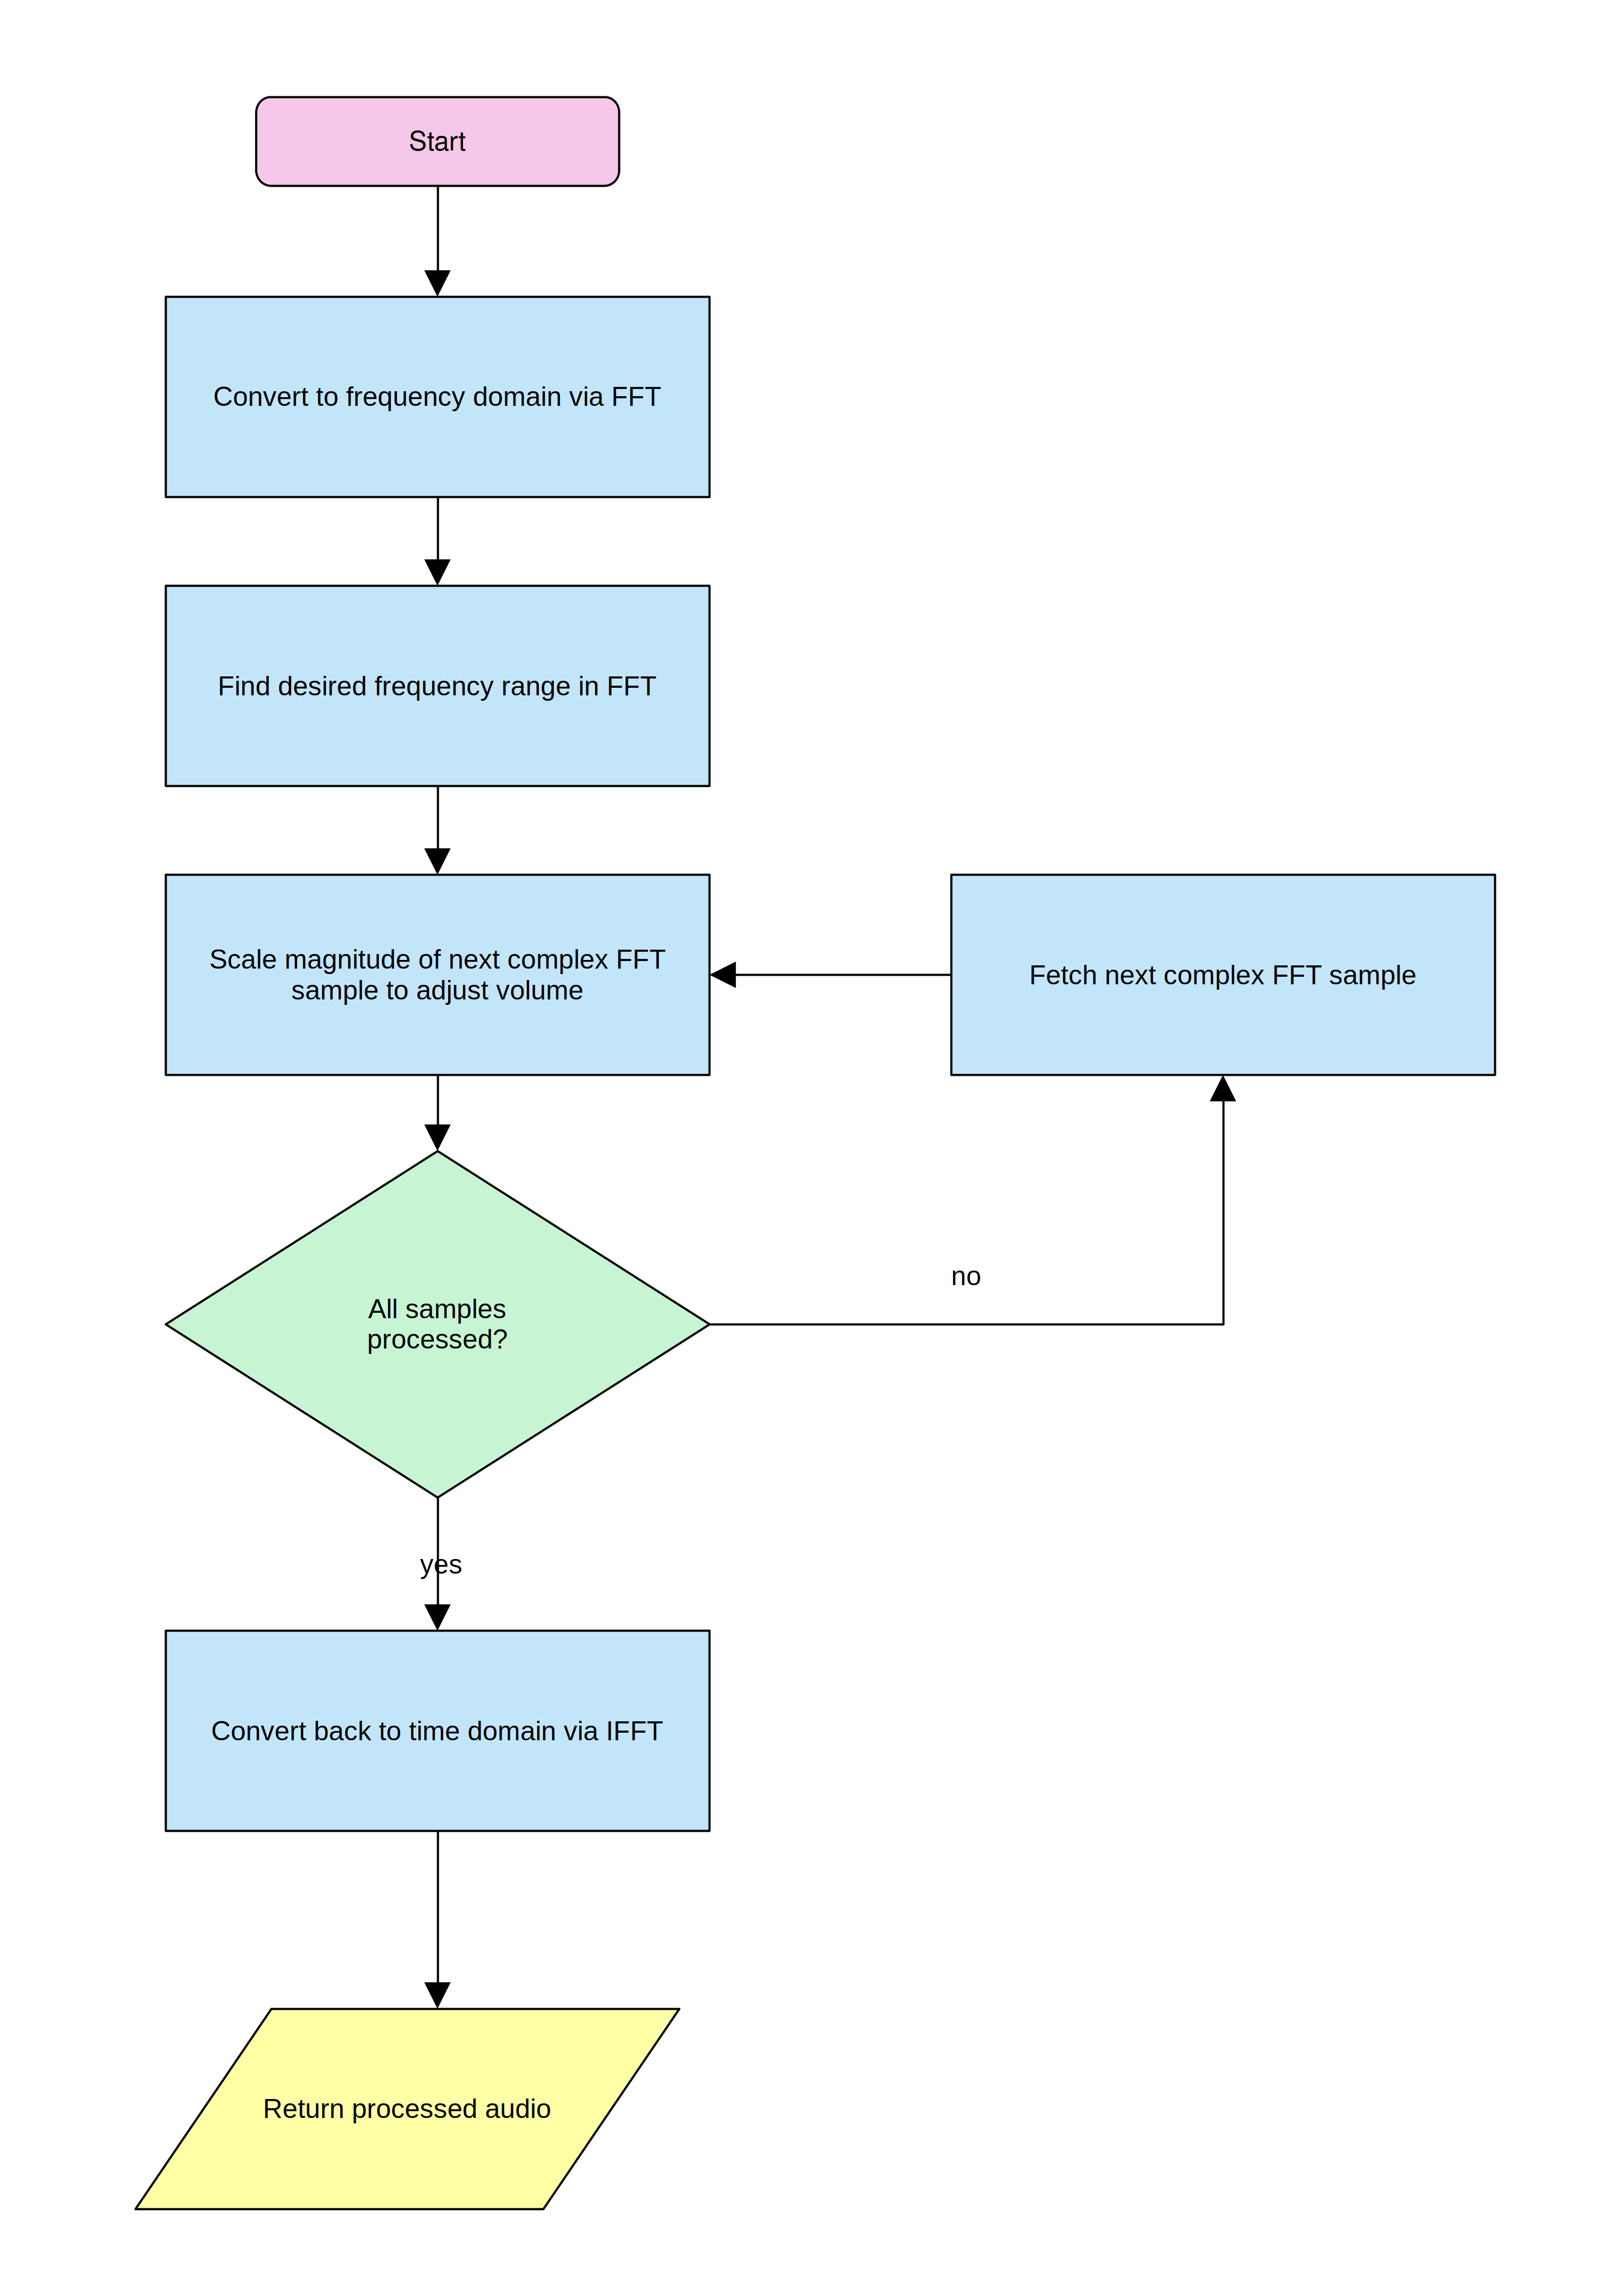
\includegraphics[width=14cm]{./equaliser flowchart.png}
	\caption{Flowchart for equaliser (frequency modification) audio effect}
\end{figure}

\begin{figure}[H]
	\subsubsection{Echo}
	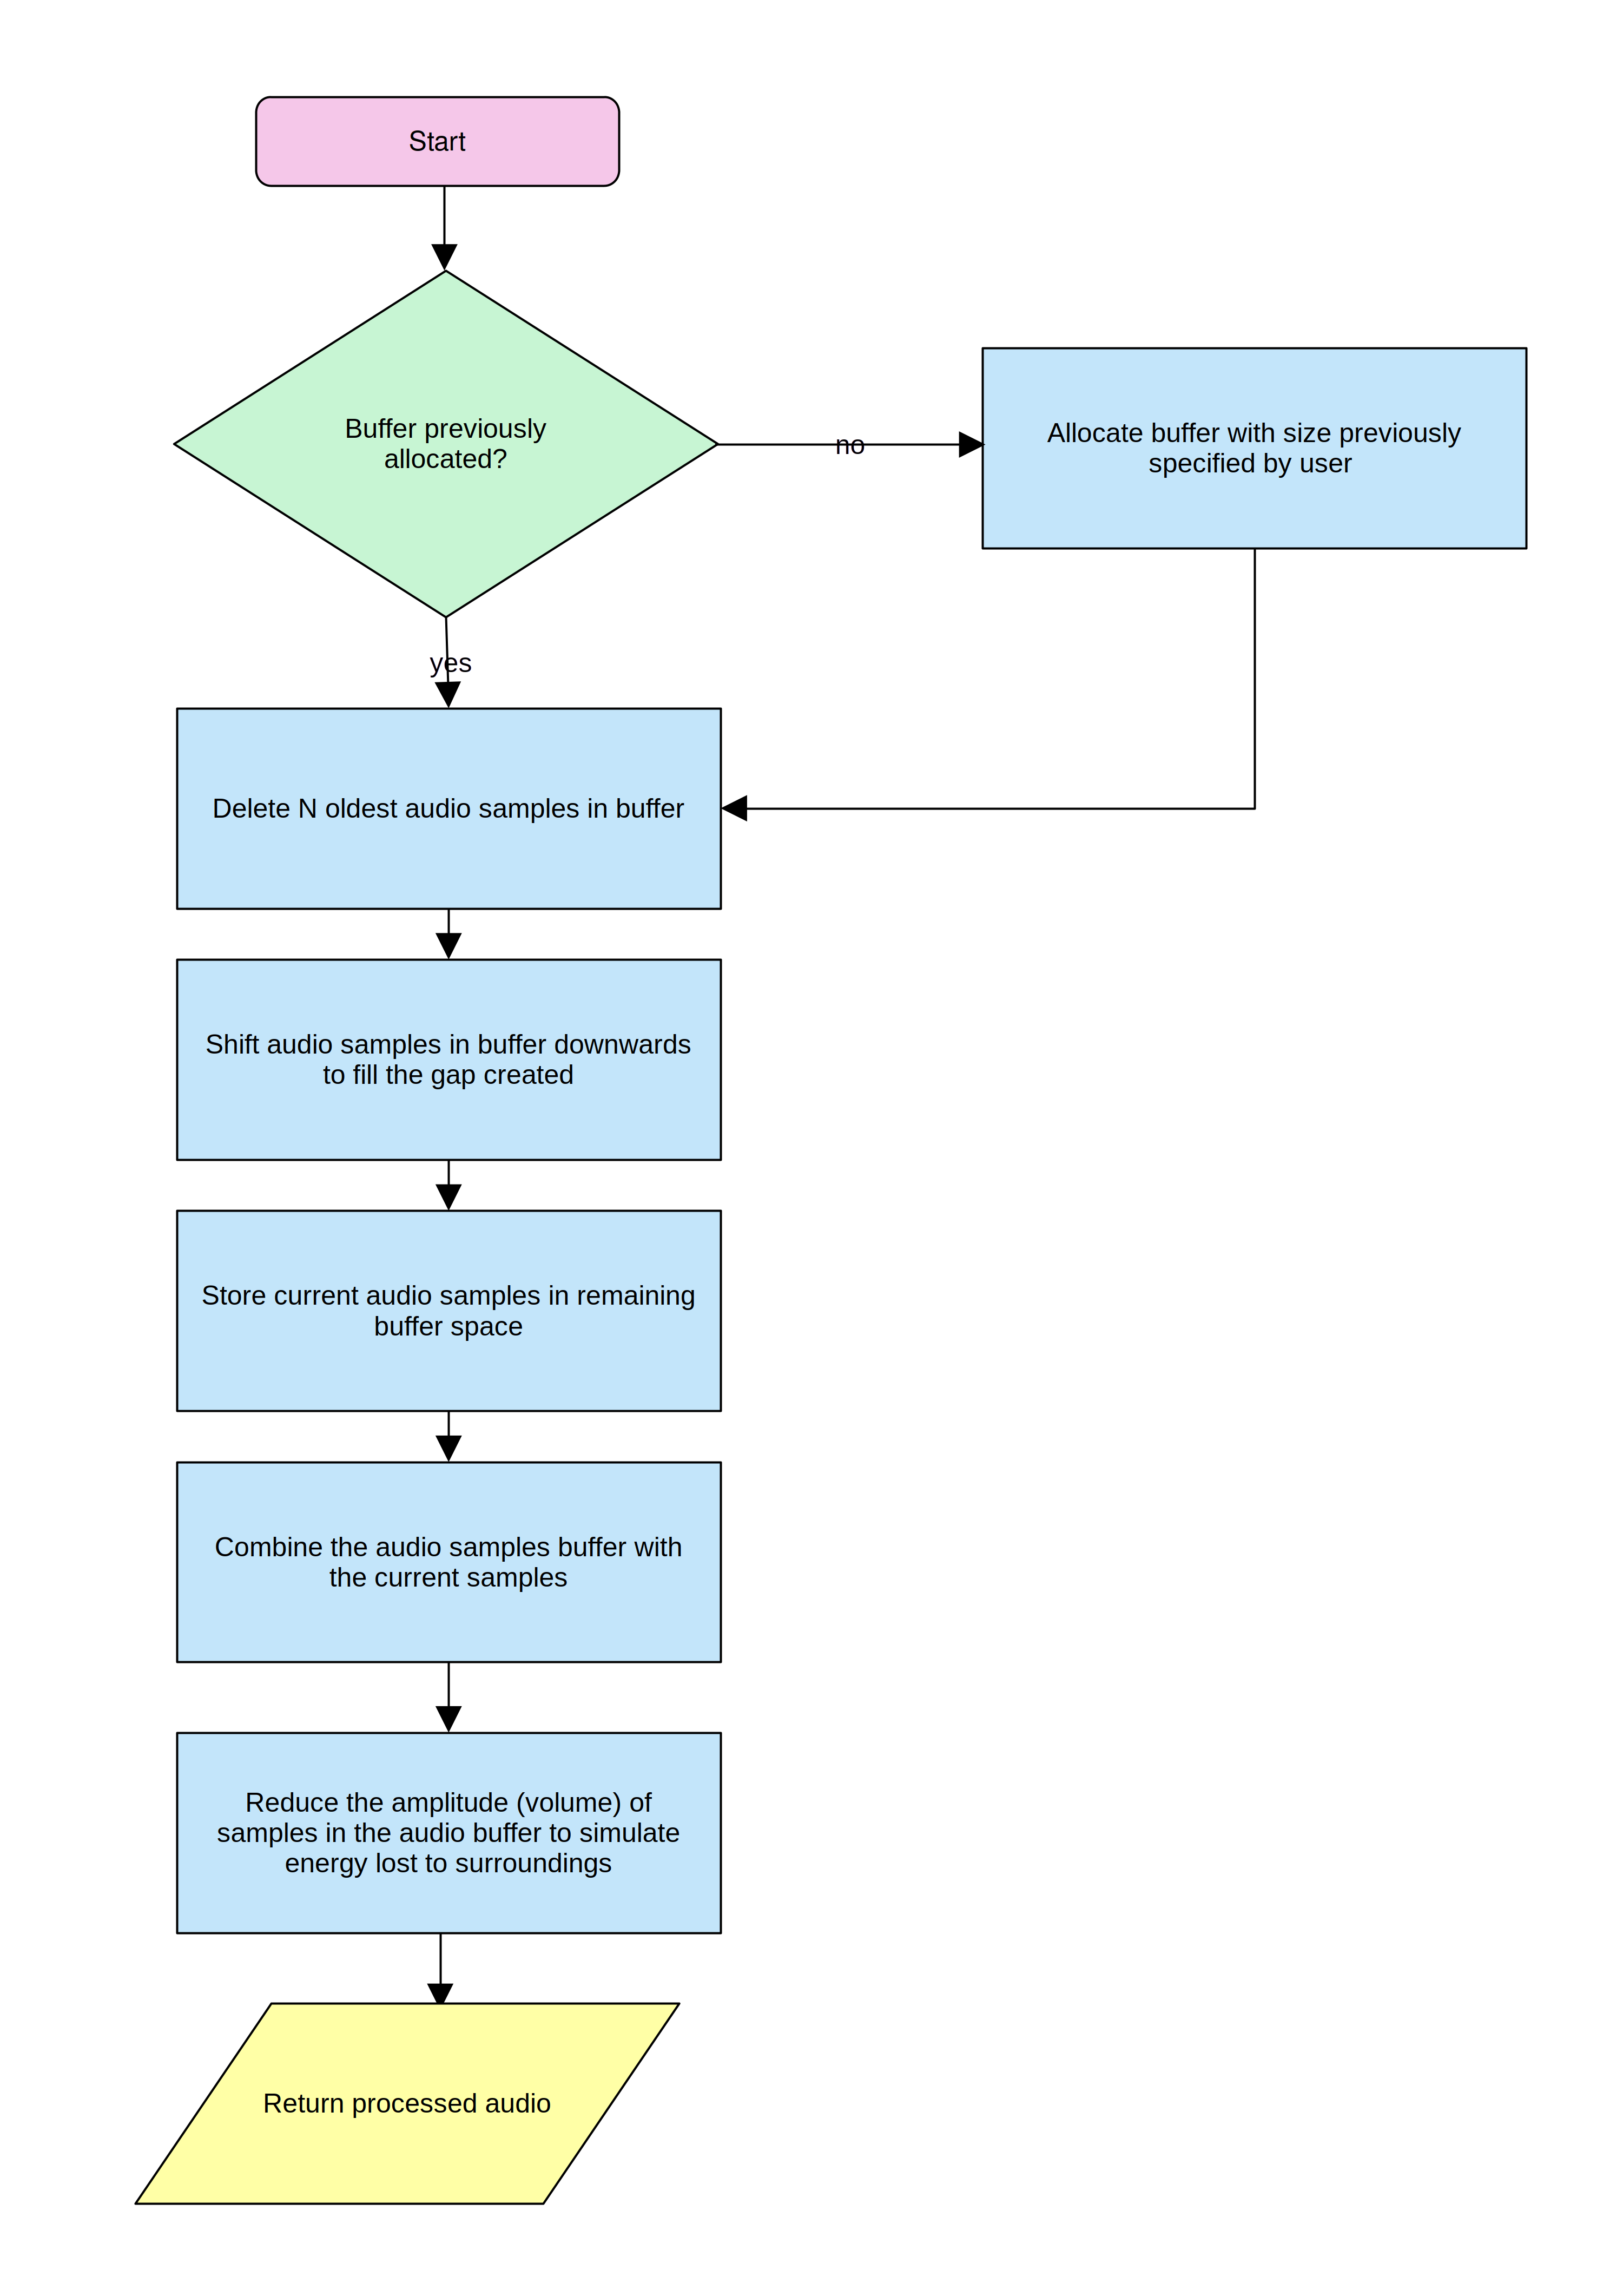
\includegraphics[width=14cm]{./echo flowchart.png}
	\caption{Flowchart for echo audio effect}
\end{figure}

\begin{figure}[H]
	\subsubsection{Volume}
	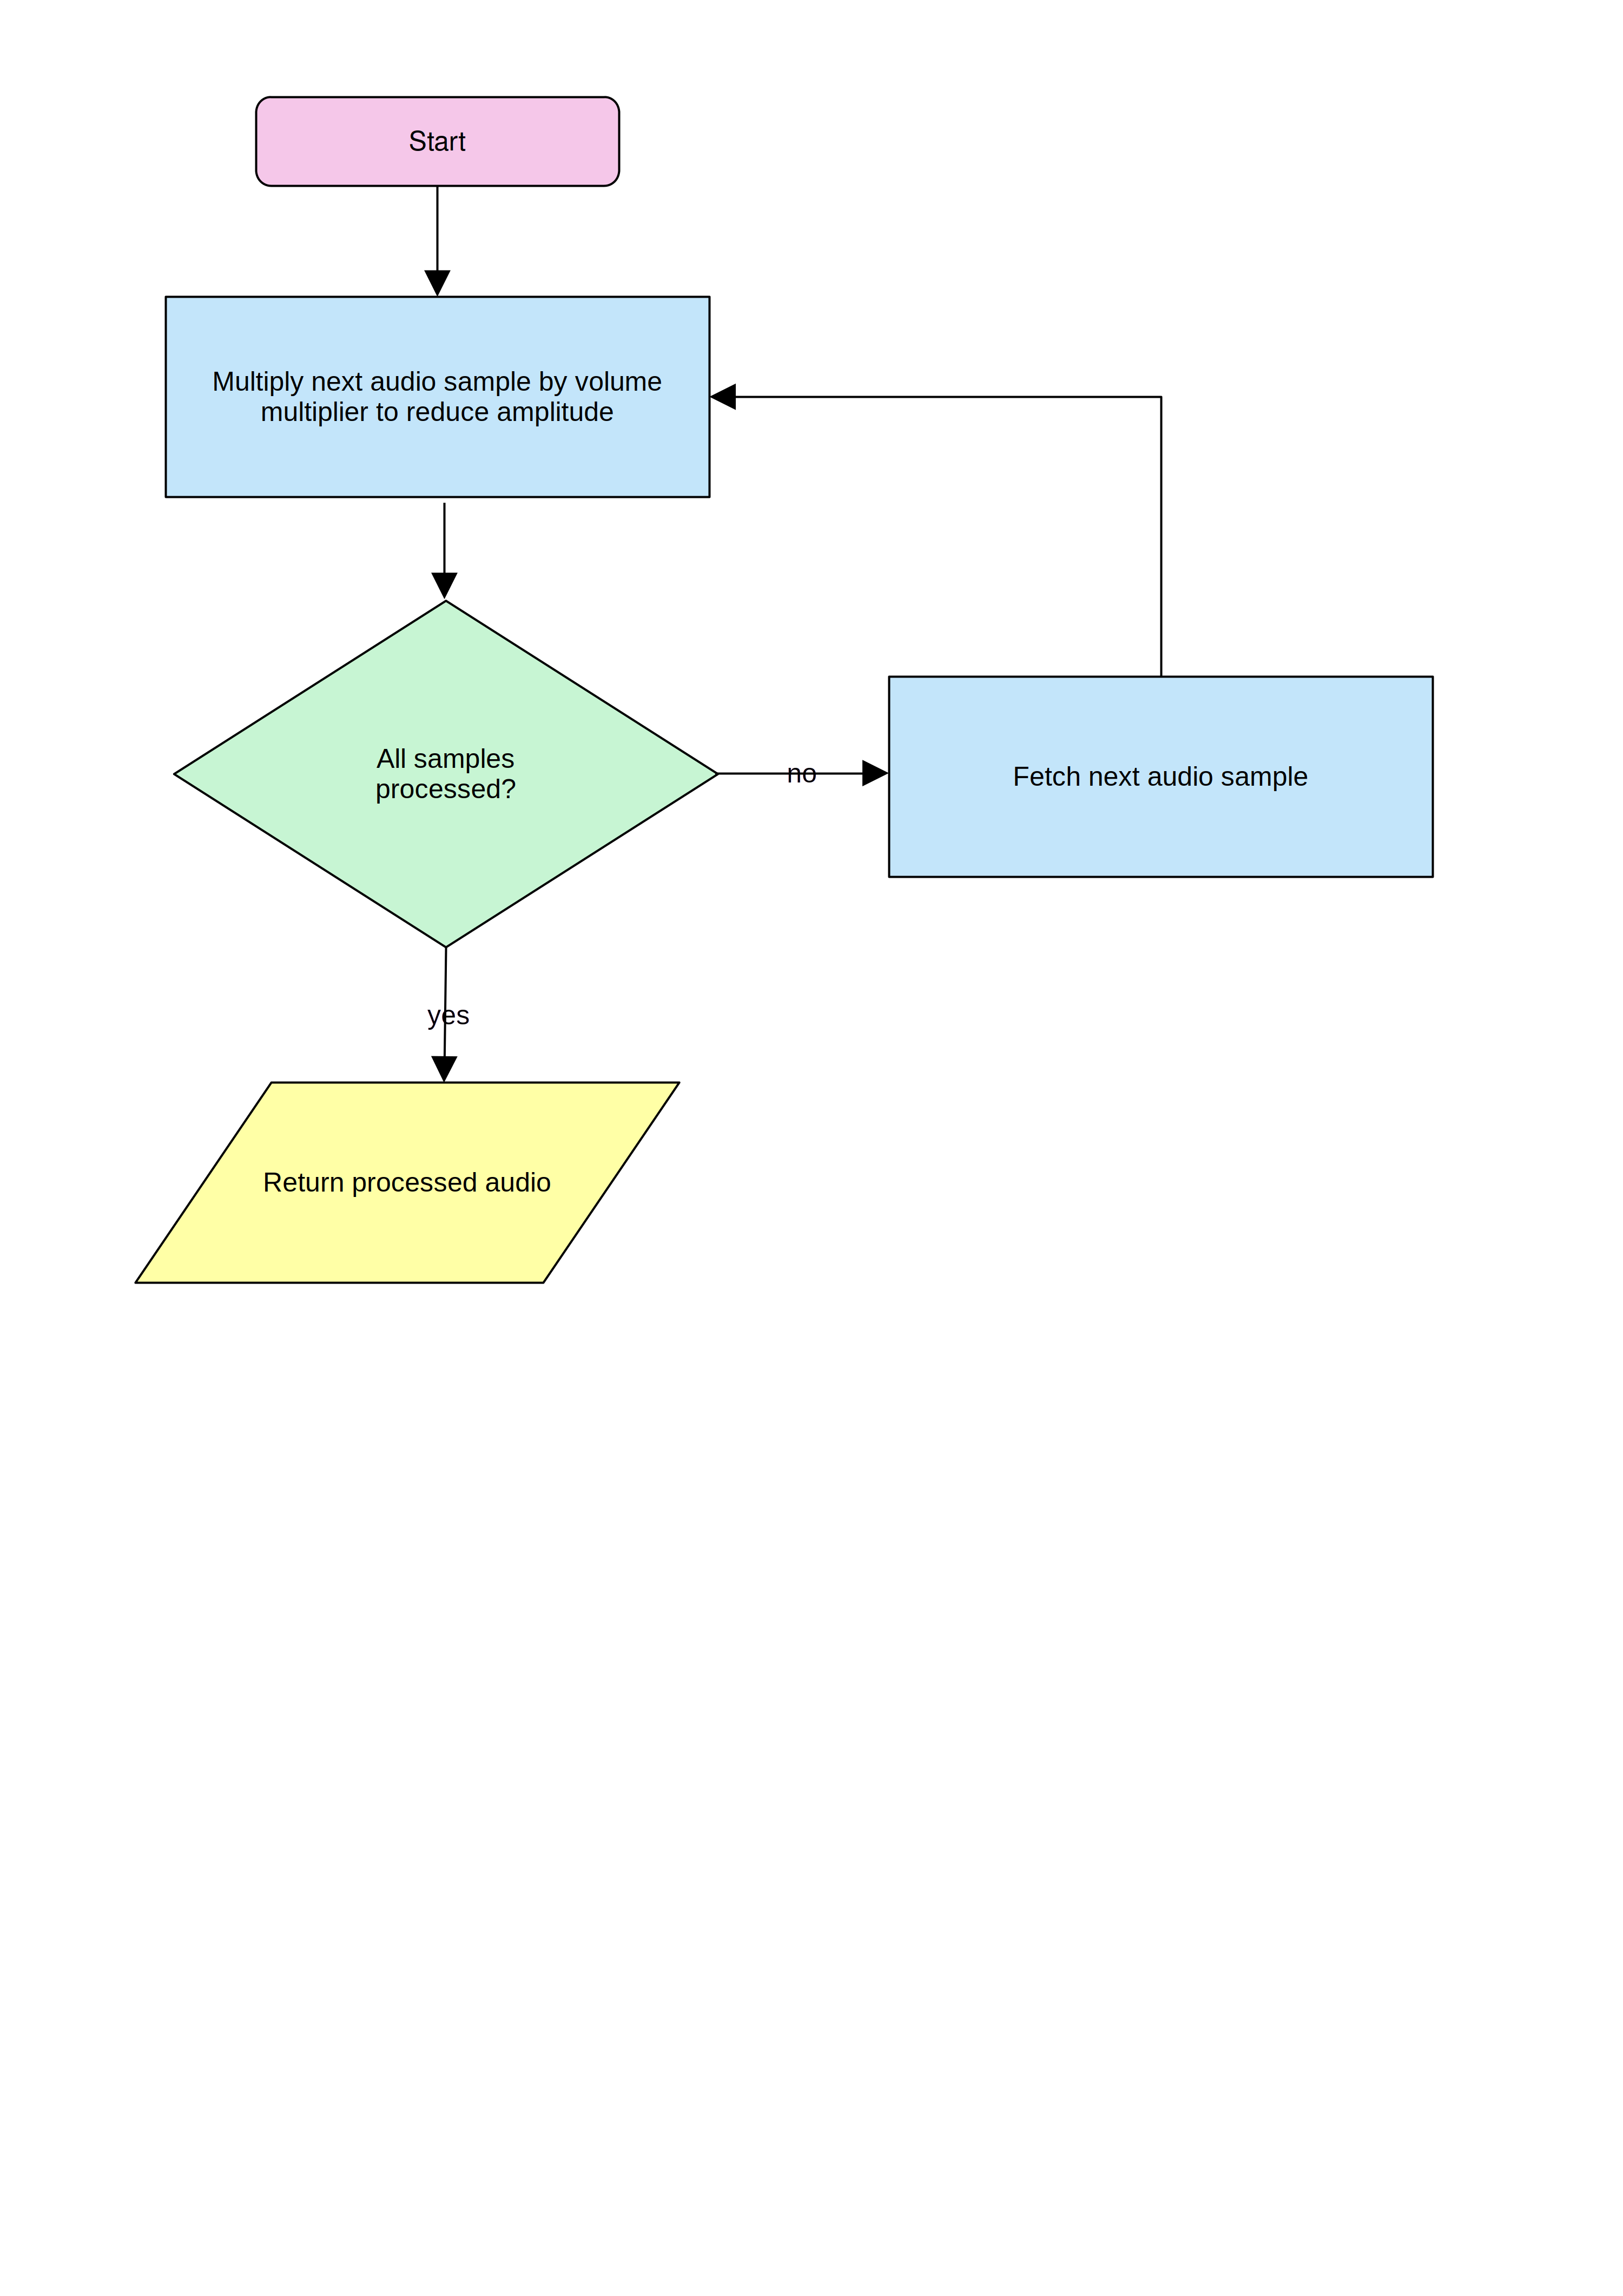
\includegraphics[width=14cm]{./volume flowchart.png}
	\caption{Flowchart for volume audio effect}
\end{figure}

\begin{figure}[H]
	\subsubsection{Noise}
	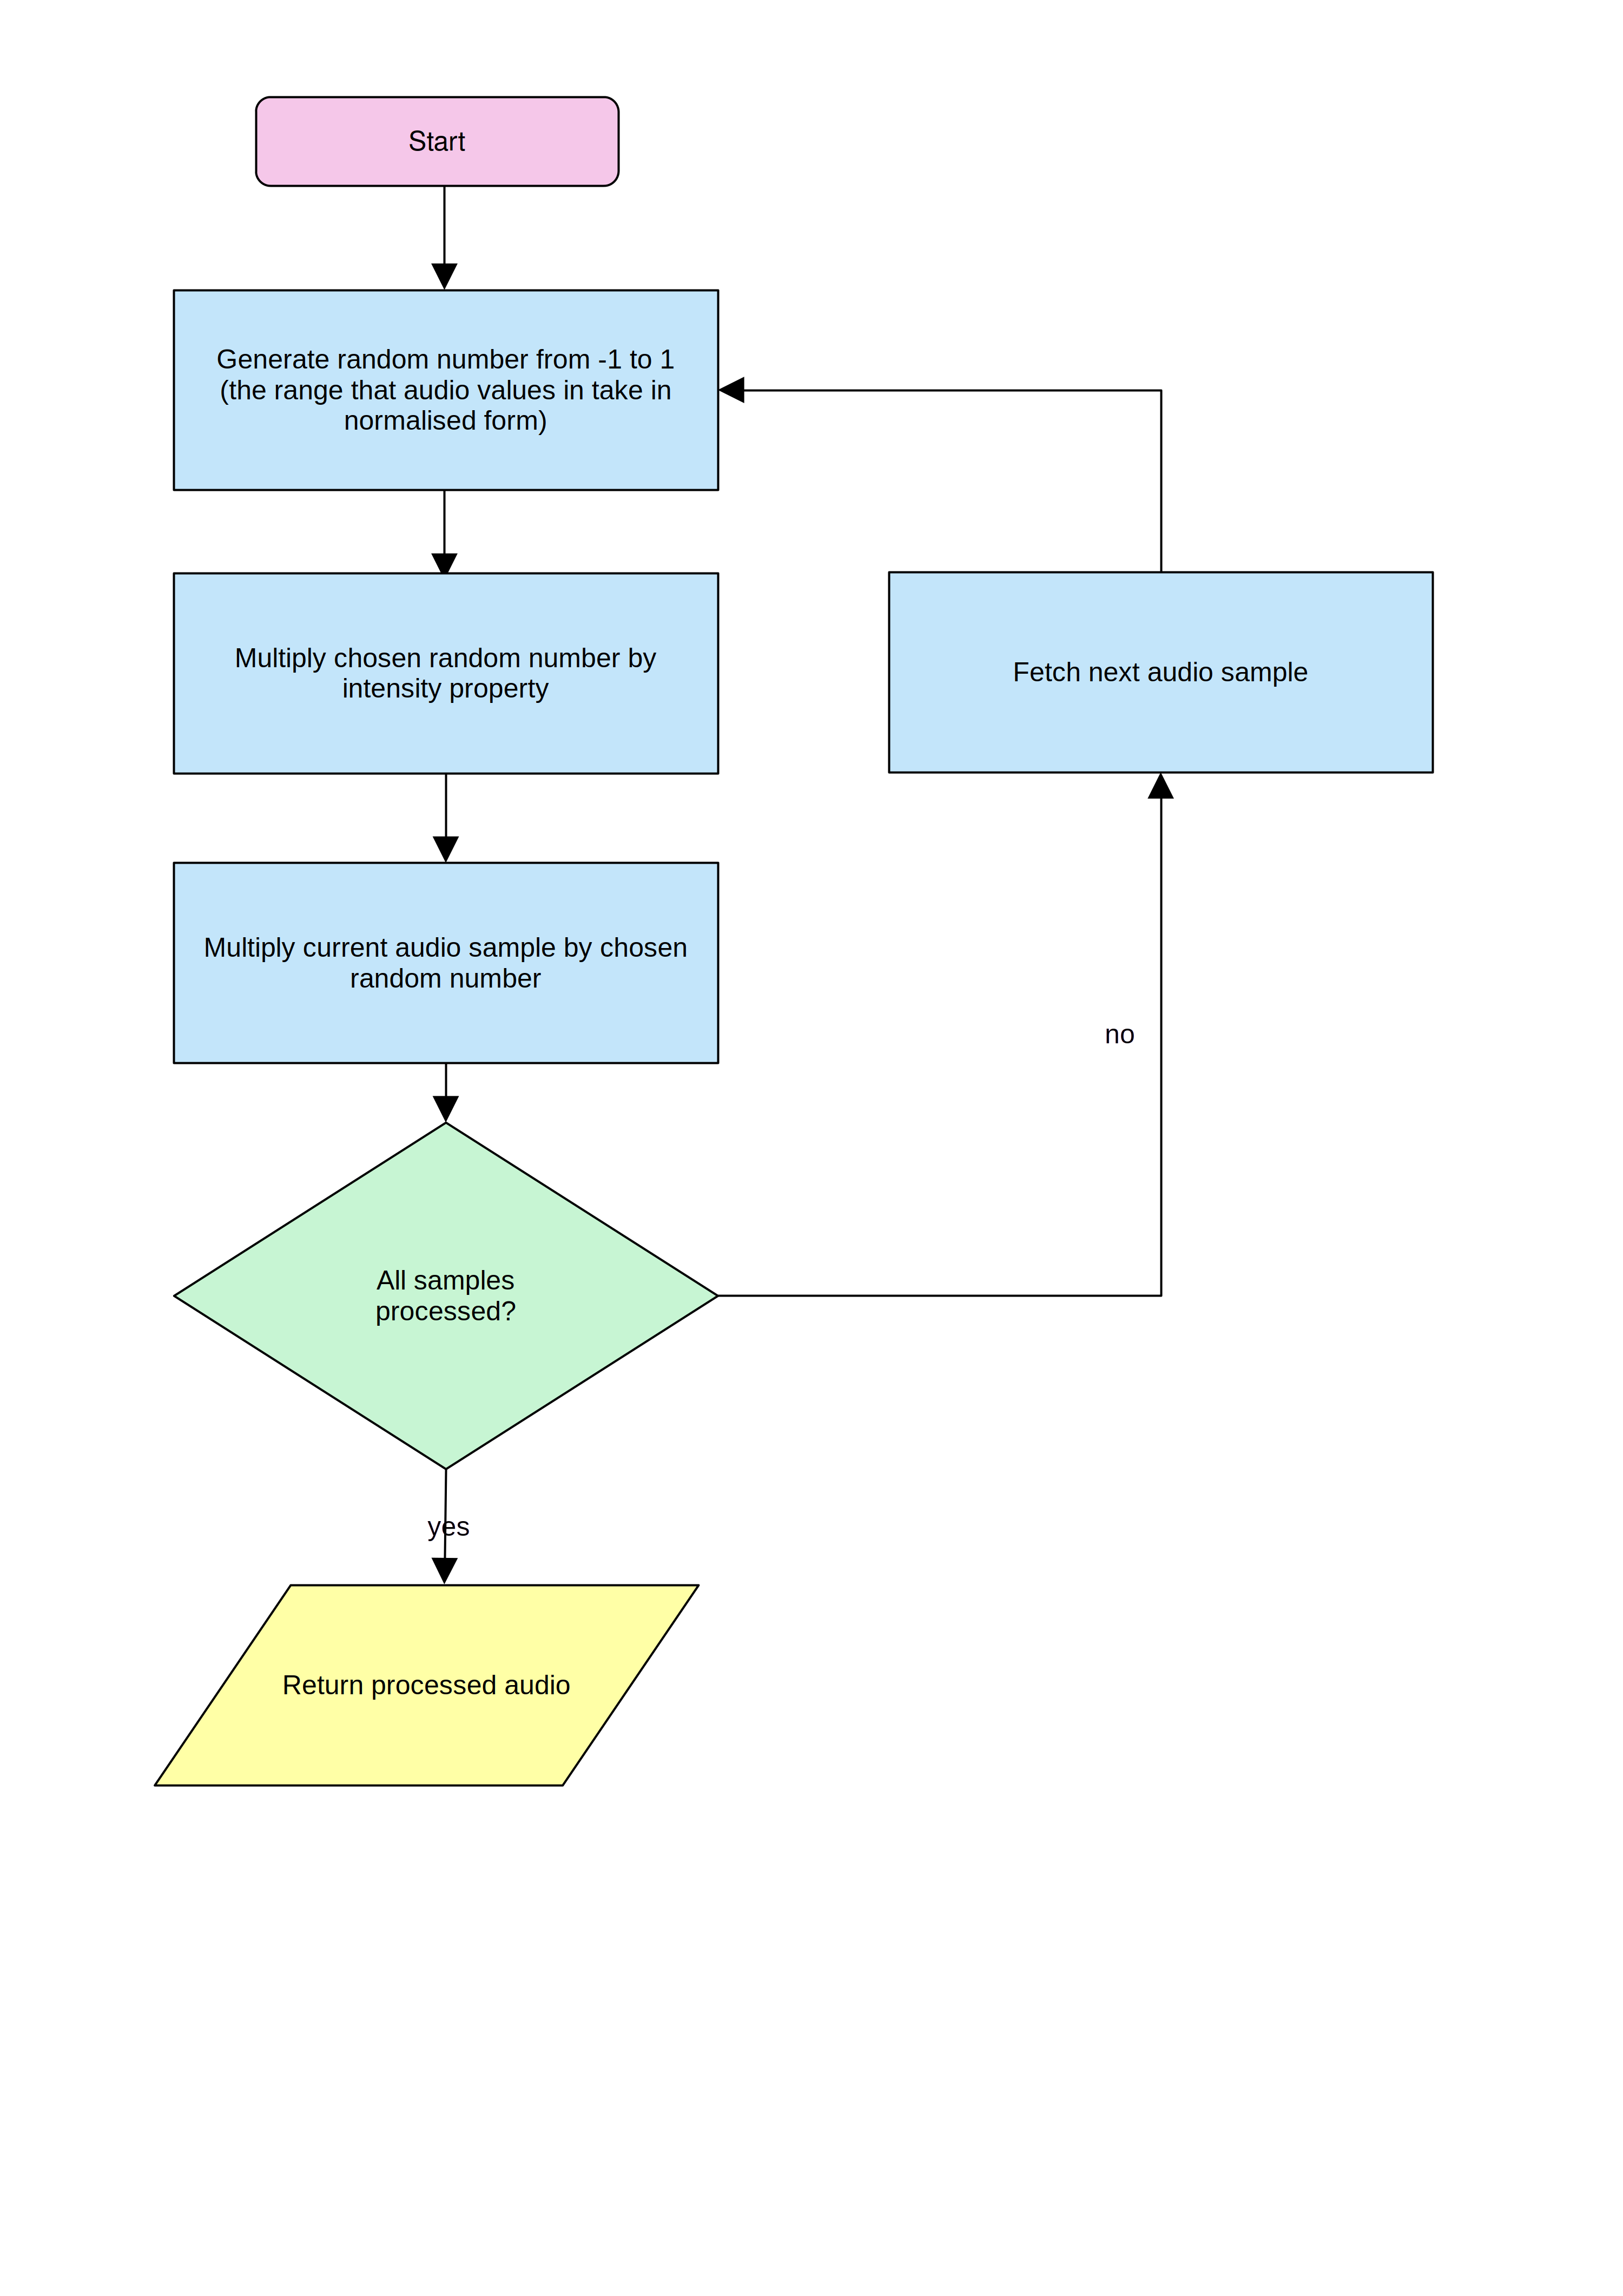
\includegraphics[width=14cm]{./noise flowchart.png}
	\caption{Flowchart for noise audio effect}
\end{figure}

\pagebreak
\subsection{Audio Visualisation and Fourier Algorithm}

\paragraph{} As can be seen in the equaliser flowchart, there is a need to perform both a Fourier Transform and an Inverse Fourier Transform on audio data in order to manipulate the audio in its frequency domain (i.e. to manipulate certain frequencies in isolation). In addition, as per the objectives outlined above, the program has a need to use this data to visualise the audio being played ("the user must be able to visualise the current audio being played in the frequency domain").

\paragraph{} Hence there is a need for pseudo-code to be designed to perform the three algorithms involved:
\begin{enumerate}
	\item A Fast Fourier Transform to convert incoming time-domain audio to its frequency-domain
	\item An algorithm that graphically displays this frequency-domain audio for the purposes of visualisation
	\item An Inverse Fast Fourier Transform to convert frequency-domain audio back to the time-domain
\end{enumerate}

\subsubsection{Cooley-Tukey FFT and IFFT Algorithm}

\paragraph{Summary of Fourier Analysis from Section 1}  Careful consideration of the problem in the analysis section revealed that acceptable performance could be achieved by using a Fast Fourier Transform (FFT), which used various mathematical techniques to reduce time complexity from \(O(N^2)\) to \(O(N\log{N})\), greatly reducing computational overhead. The most popular FFT algorithm, the "Cooley-Tukey"  FFT, was chosen, due to its use of recursion to both efficiently  and elegantly perform the computations required.

\paragraph{Comparing the FFT and IFFT}
It should be stressed that there is very little difference between performing a "normal" Fast Fourier Transform using the Cooley-Tukey algorithm and an \textit{inverse} Fast Fourier Transform. For this reason, I have decided to combine the two into a single function to eliminate as much code duplication as possible.

\pagebreak
\paragraph{Pseudo-code implementation of algorithm}
\begin{minted}{ada}
-- Converts an array of floats (i.e. the audio samples) into an array of complex numbers
-- by using 0 for the imaginary parts. We must check the incoming data is a power of 2
-- as later code that uses the results of this computation (i.e. the FFT) depends on this.
function convert_samples_to_complex_form(samples: array of float) -> array of complex:
	if size of samples is not a power of 2:
		raise error "FFT data has invalid size"

	complex_samples := new array of complex with size equal to size of samples
	for each sample in samples:
		append (sample, 0.0) as a complex number to complex_samples

	return complex_samples

-- Performs both either an FFT or an IFFT recursively by diving the data into two
-- until the trivial base case is reached
function do_fft(input: reference to array of complex, mode: Mode):
	N := size of input
	if N <= 1:
		return

	-- Split data by even and odd indices
	even := new array of complex with size N/2
	odd := new array of complex with size N/2
	for i from 0 to N/2 - 1:
		even[i] := input[2*i]
		odd[i] := input[2*i + 1]

	-- Perform FFT / IFFT recursively on even and odd halves
	do_fft(even, mode)
	do_fft(odd, mode)

	for k from 0 to N/2 - 1:
		-- Perform FFT calculation by manipulating audio sample in the complex plane
		-- as per the formal defition (see analysis section)
		sign := if mode is Normal then -1.0 else 1.0
		t := polar(1.0, sign * 2.0 * PI * k / N) * odd[k]
		input[k] := even[k] + t
		input[k + N/2] := even[k] - t

-- Example code for using FFT
incoming_audio = fetch_upcoming_audio_data_from_buffer()
complex_audio = convert_samples_to_complex_form(incoming_audio)
do_fft(complex_audio, Mode::Normal)

-- (calculations on frequency domain, including visualisation, performed here)

-- Convert back to time domain (example code using IFFT)
do_fft(fft_result, Mode::Inverse)
final_audio = discard_imaginary_parts_of_complex_array(complex_audio)
submit_audio_to_speakers(final_audio)
\end{minted}

\pagebreak
\subsubsection{Visualisation Algorithm}

\paragraph{Interpreting the results of an FFT}
After an FFT has been performed, the resultant frequency-domain data needs to be visualised. The data returned from an FFT is an array of complex numbers where each index corresponds to a particular range of frequencies. The amplitude of these frequencies is just the magnitude of the complex number at that index. For example, index 12 might correspond to frequencies from 100 Hz to 130 Hz, and the magnitude of the complex number at fft\_array[12] would be the amplitude.

\paragraph{}
The range of frequencies each element in the FFT data represents is called the "frequency resolution", whereby:
\[
\text{frequency resolution} = \frac{\text{frequency of incoming audio}}{\text{number of samples in audio provided to FFT algorithm}}
\]

\paragraph{}
Hence for any given index in the array, the minimum frequency it represents is given by:
\[
	\text{min frequency} = \text{index in the array} \times \text{frequency resolution}
\]

\paragraph{}
The visualisation I have chosen is a bar chart, where the x-axis represents frequency and the y-axis represents amplitude. Each bar can be said to have:
\begin{itemize}
	\item a minimum frequency
	\item a maximum frequency
	\item an amplitude
\end{itemize}
Hence an algorithm is needed to convert the incoming FFT frequency-domain data into the above format for later rendering. The minimum and maximum frequencies can be derived from the equations above.

\paragraph{Using a non-uniform scale for frequency}
The human ear does not perceive frequencies in a linear fashion. In other words, if one adds 500 Hz to a sound-wave repeatedly, the "jump" in pitch will not always sound the same.  This is because human-hearing follows a roughly logarithmic scale when it comes to detecting frequencies. This represents a problem as using a uniform, linear scale on the visualisation bar chart, whilst mathematically correct, will not sound plausible to the ear. Instead, the x-axis (frequency) for the bar chart must be adjusted so that, relative to the human ear, each bar represents roughly the same jump in \textit{perceived} pitch. The most suitable scale for this is the "Bark scale", where "equal distances correspond with perceptually equal distances" as described above. A frequency can be converted into its Bark equivalent using a simple formula:
\[
\text{Bark} = 13 \arctan(0.00076 \times \text{frequency}) + 3.5 \arctan ((\text{frequency} / 7500)^2)
\]

\paragraph{Using a non-uniform scale for amplitude}
Just like with frequency, the human ears perceive amplitude logarithmically too. If a sound-wave has twice the frequency, it will not necessarily sound twice as loud. Thus the y-axis of the bar chart must be adjusted to reflect the \textit{perceived} loudness. A good  approximation is to take each amplitude and log it to base 10.

\paragraph{Ignoring inaudible sounds}
The human ear cannot hear sounds below 20 Hz or above 20,000 Hz. These frequencies should therefore be ignored in the visualisation, and hence the algorithm should be able to reject frequencies outside a specified frequency,

\pagebreak
\begin{minted}{ada}
function hertz_to_bark_scale(hertz: float) -> float:
	return 13.0 * arctan(0.00076 * hertz) + 3.5 * arctan((hertz / 7500.0) * (hertz / 7500.0))

-- GroupSettings is a data structure consiting of the number of samples ("buckets") provided to the FFT,
-- the frequency of the incoming audio, and the minimum and maximum  acceptable frequencies.
function convert_fft_to_bar_chart_format(fft: array of complex, group_settings: GroupingSettings) -> array of FrequencyRange:

	-- Work out frequency resolution
	n_samples := size of fft
	frequency_resolution := group_settings.frequency / n_samples

	-- Work out min and max frequencies in Bark scale and distance between "buckets"
	minimum_frequency_bark := hertz_to_bark_scale(group_settings.minimum_audible_frequency)
	maximum_frequency_bark := hertz_to_bark_scale(group_settings.maximum_audible_frequency)
	bark_distance := (maximum_frequency_bark - minimum_frequency_bark) / group_settings.n_buckets

	buckets := new array of float with size equal to group_settings.n_buckets, initialized with zeros

	-- The FFT is symmetrical (because audio data lies only on the real axis), so we actually only  need
	-- to visualise the first half of it
	for i from 0 to (n_samples/2 - 1):
		frequency := i * frequency_resolution
		if frequency >= group_settings.minimum_audible_frequency
		  and frequency <= group_settings.maximum_audible_frequency:

			-- Use Bark scale conversion to work out location of "bar" in bar chart
			bark_frequency := HertzToBarkScale(frequency)
			index := (bark_frequency - minimum_frequency_bark) / bark_distance

			if index < size of buckets:
				-- Calculate amplitude of frequency (i.e. the magnitude of the complex number)
				-- Add this to the height of the bar at this point in the bar chart
				buckets[index] += absolute value of fft[i]

	-- Work out maximum amplitude in bar chart
	max_magnitude := 0.0
	for each bucket in buckets:
		if bucket > max_magnitude:
			max_magnitude := bucket

	-- Scale magnitudes logarithmically
	for each bucket in buckets:
		bucket := logarithm base 10 of (1.0 + bucket / max_magnitude)

	-- Convert bucket array (raw bar chart data) into a more usable format
	ranges := new array of FrequencyRange with size equal to size of buckets
	for i from 0 to size of buckets - 1:
		lower_freq := minimum_frequency_bark + (i + 0.0) * bark_distance
		upper_freq := maximum_frequency_bark + (i + 1.0) * bark_distance

		-- Convert back to Hertz scale
		lower_freq := 0.5 + 600.0 * sinh(lower_freq / 6.0)
		upper_freq := 0.5 + 600.0 * sinh(upper_freq / 6.0)

		ranges[i] := FrequencyRange {
			min_frequency: integer part of lower_freq,
			max_frequency: integer part of upper_freq,
			magnitude: buckets[i]
		}

	return ranges
\end{minted}
\pagebreak
\begin{minted}{ada}
function draw_bar_chart(bars: array of FrequencyRange):
	draw_screen_background()

	-- Find max magnitude
	max_magnitude := 0.0
	for i from 0 to size of bars - 1:
		if (bars[i].magnitude > max_magnitude)
			max_magnitude = bars[i].magnitude

	-- Work out scaling
	bar_width := screen_width / (size of bars)
	bar_height_scale := screen_heigh / max_magnitude

	for i from 0 to size of bars - 1:
		bar_height = bars[i].magnitude * bar_height_scale
		draw_rectangle(
			x: i * bar_width,
			y: 0,
			width: bar_width,
			height: bar_height
		)
\end{minted}

\pagebreak

\pagebreak
\subsection{Program GUI}

\paragraph{}
The user will interact with the program using a GUI. In order to maximise the potential user-base, I have decided to use a popular C++ GUI library called "wxWidgets", which allows for the creation of GUIs using a singular code-base for Windows, Linux and MacOS, amongst others.

\subsubsection{GUI "screens"}
The user will navigate through a variety of "screens" in order to use the program. The GUI flow can be modelled as followed:
\begin{itemize}
	\item When the program starts, the user must chose to either load an existing playlist (see "Audio Data and Playback"), or create a new one - this is the "choice screen".
	\item Should the user chose to create a playlist, a new "screen" will be displayed where they can append audio files on the system to a playlist, before saving it.
	\item Returning back to the initial "choice screen", the user will then chose to load their existing playlist, or optionally create another one for later use.
	\item After a playlist has been selected, the main "playback screen" will be displayed. Audio playback will begin.
	\item The user can view the current audio visualisation, as well as audio playback progress.
	\item A menu will allow the user to configure the current playback and visualisation, such as by adding new audio effects or changing the visualisation settings.
	\item A separate "screen" can be displayed allowing the user to view current audio effects.
	\item In this screen, if a user chooses to edit a current audio effect, a new screen will be displayed, showing the various options one can adjust.
\end{itemize}

\paragraph{Summary of "screens"}
\begin{itemize}
	\item "Choice" screen (create new playlist or load existing one)
	\item "Create playlist" screen
	\item "Playback" screen
	\item "Effects list" screen
	\item "Edit effect" screen
\end{itemize}

\paragraph{Popups}
Minor tasks such as  selecting a new song from a playlist or modifying visualisation settings will be handled with popup dialogue menus.

\begin{figure}[H]
	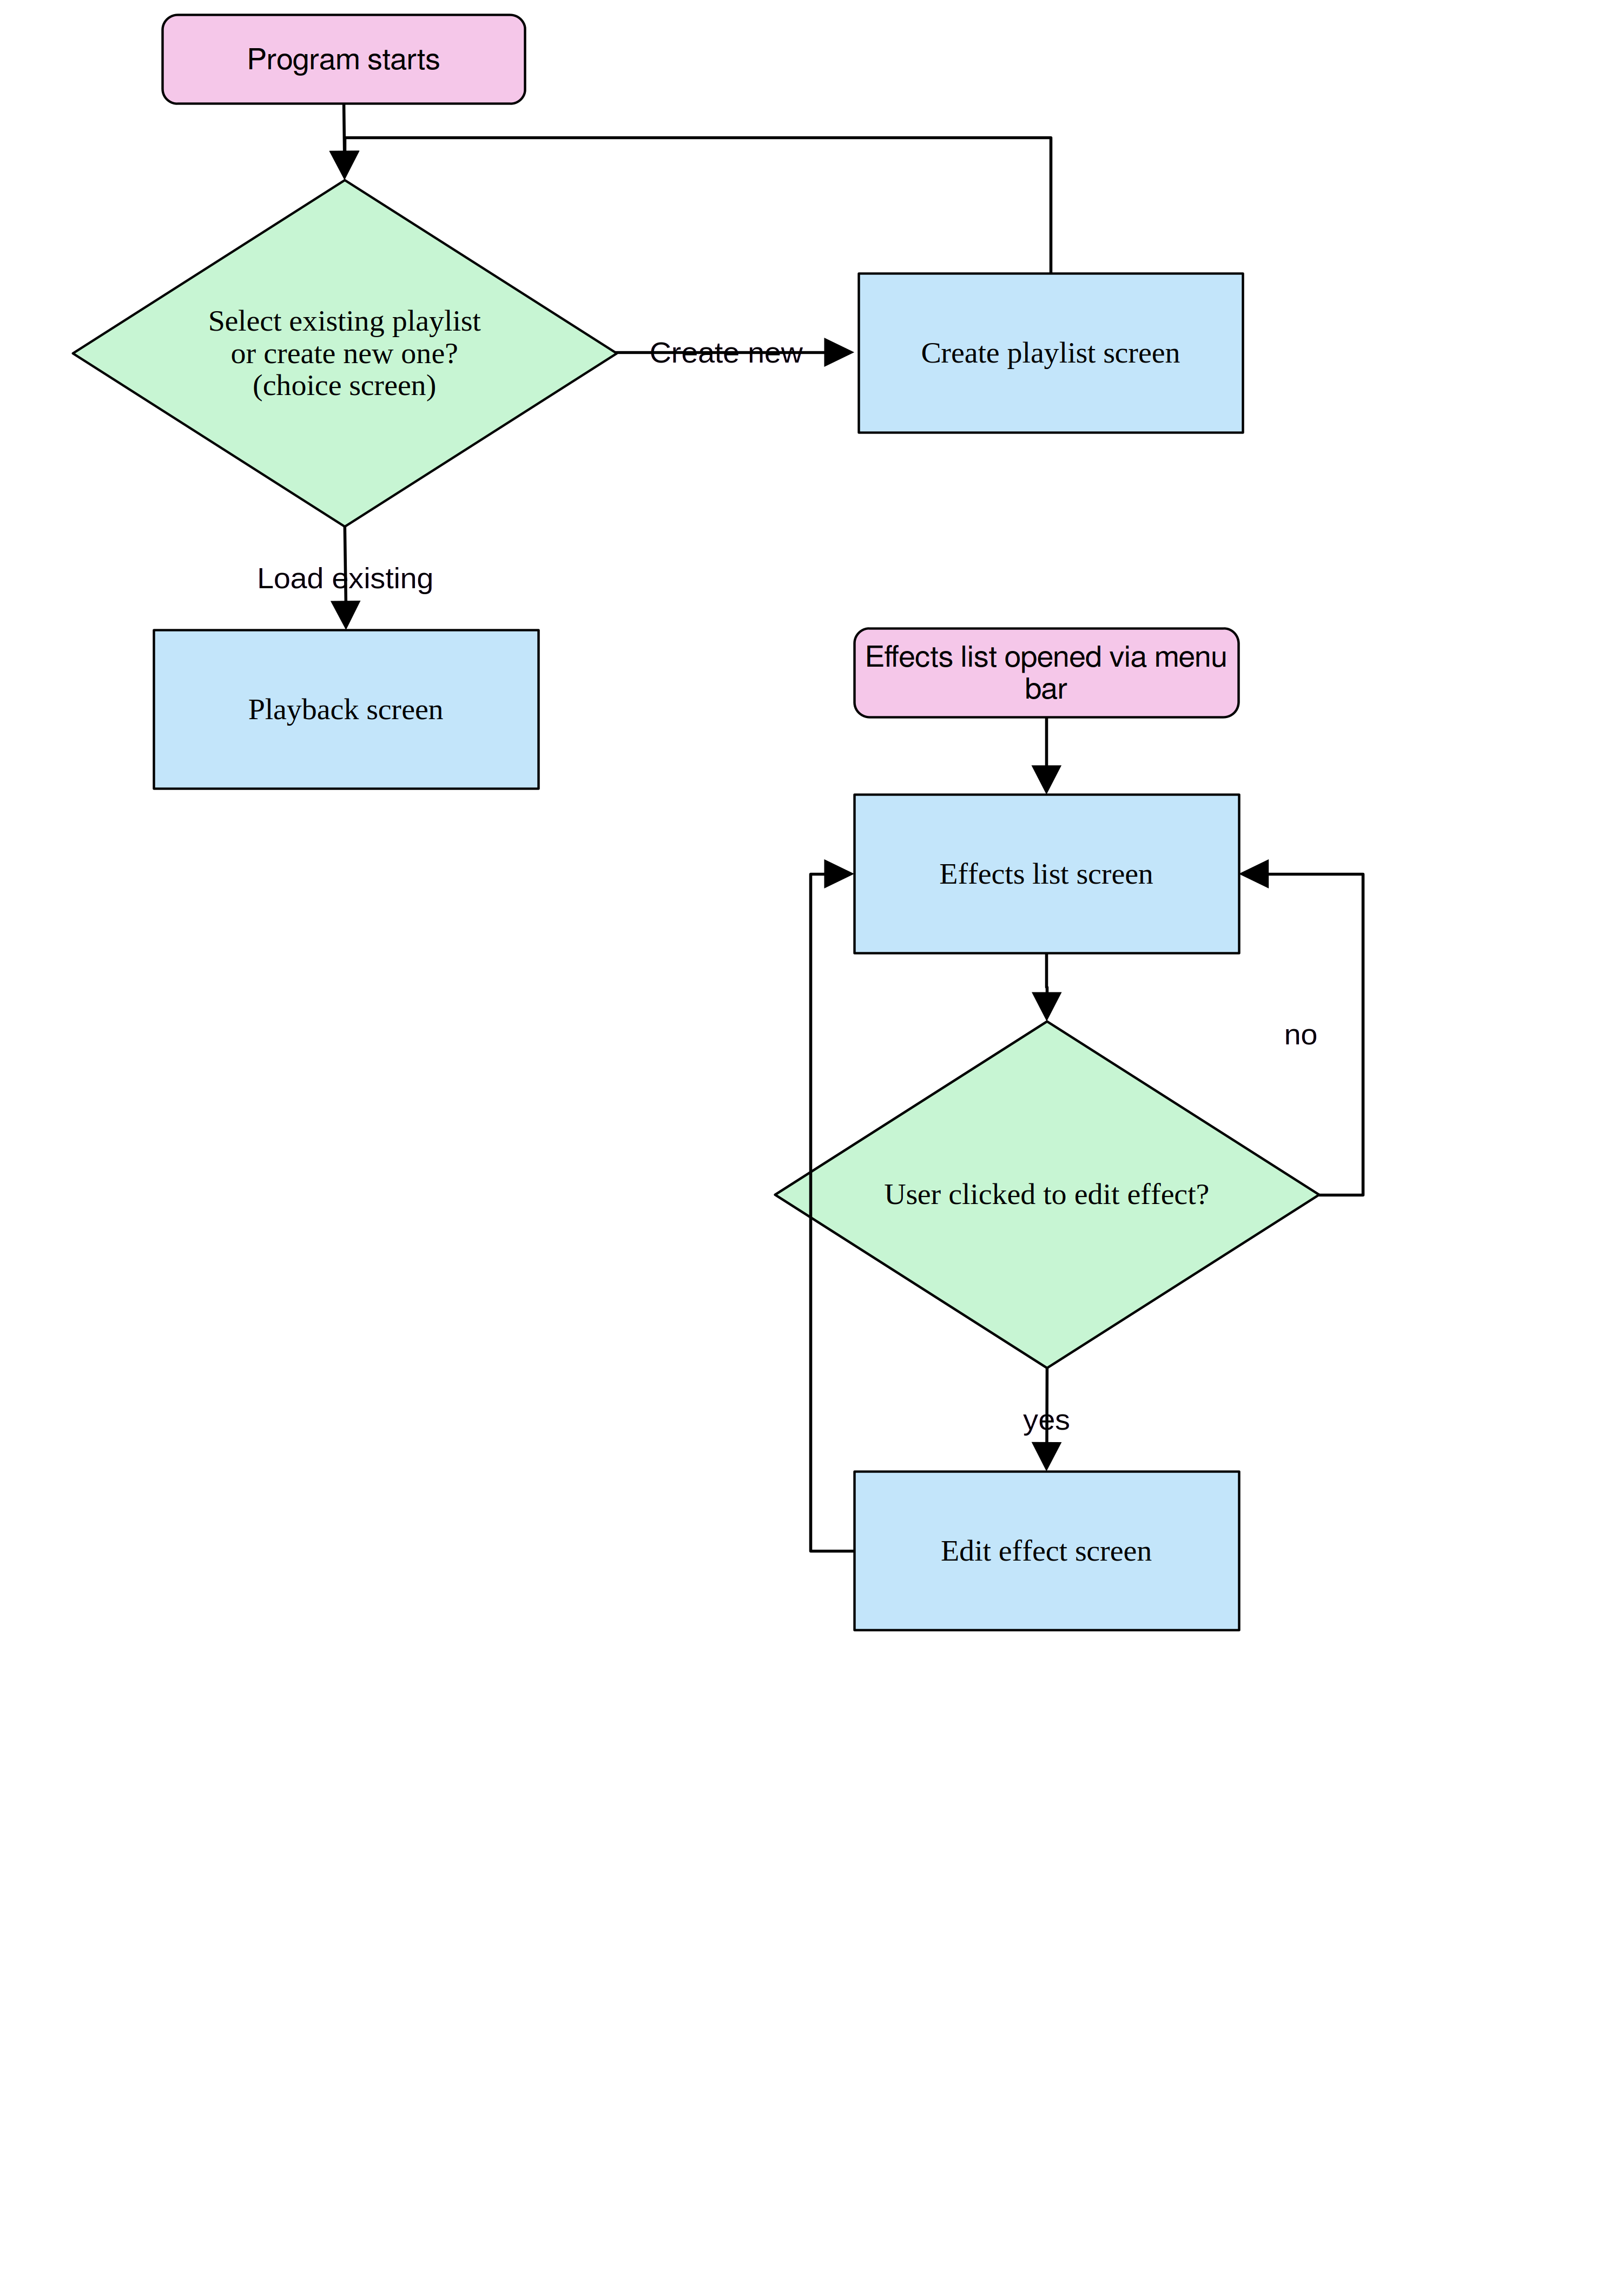
\includegraphics[width=14cm]{./gui flow.png}
	\caption{GUI flow for program }
\end{figure}

\subsubsection{GUI Wireframes}

\begin{figure}[H]
	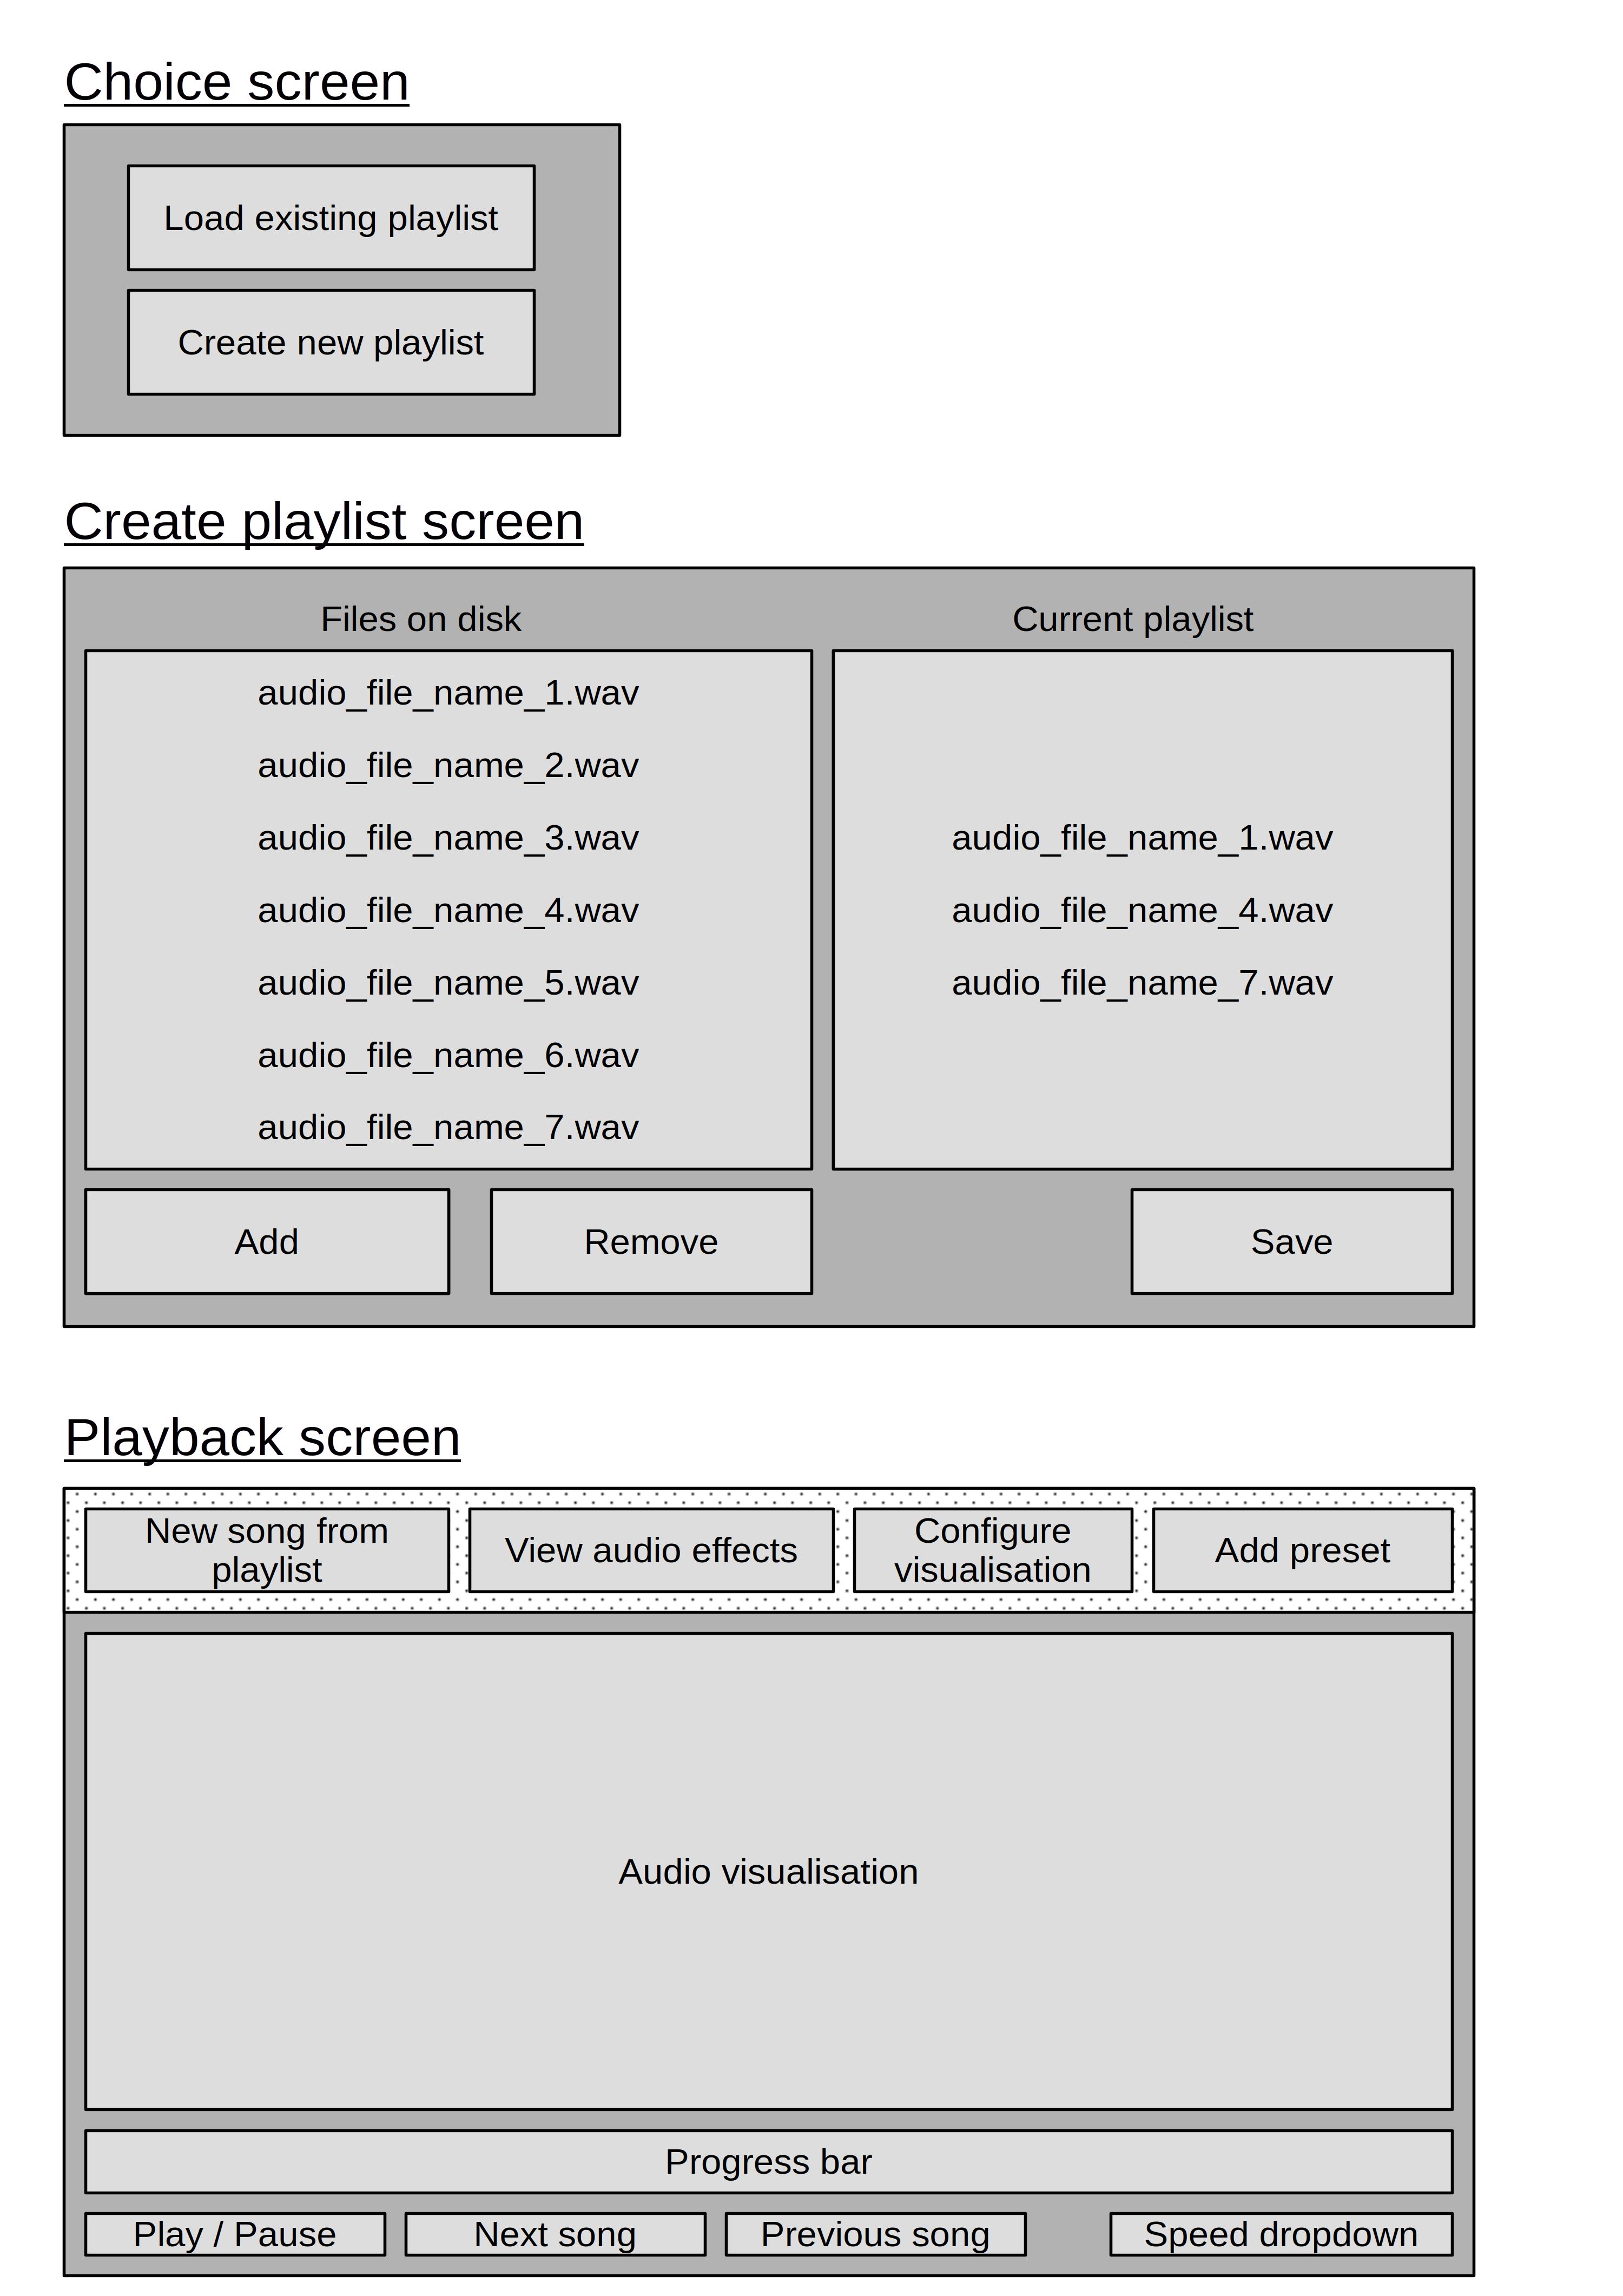
\includegraphics[width=14cm]{./gui wireframes one.png}
	\caption{GUI wireframes for main windows }
\end{figure}

\begin{figure}[H]
	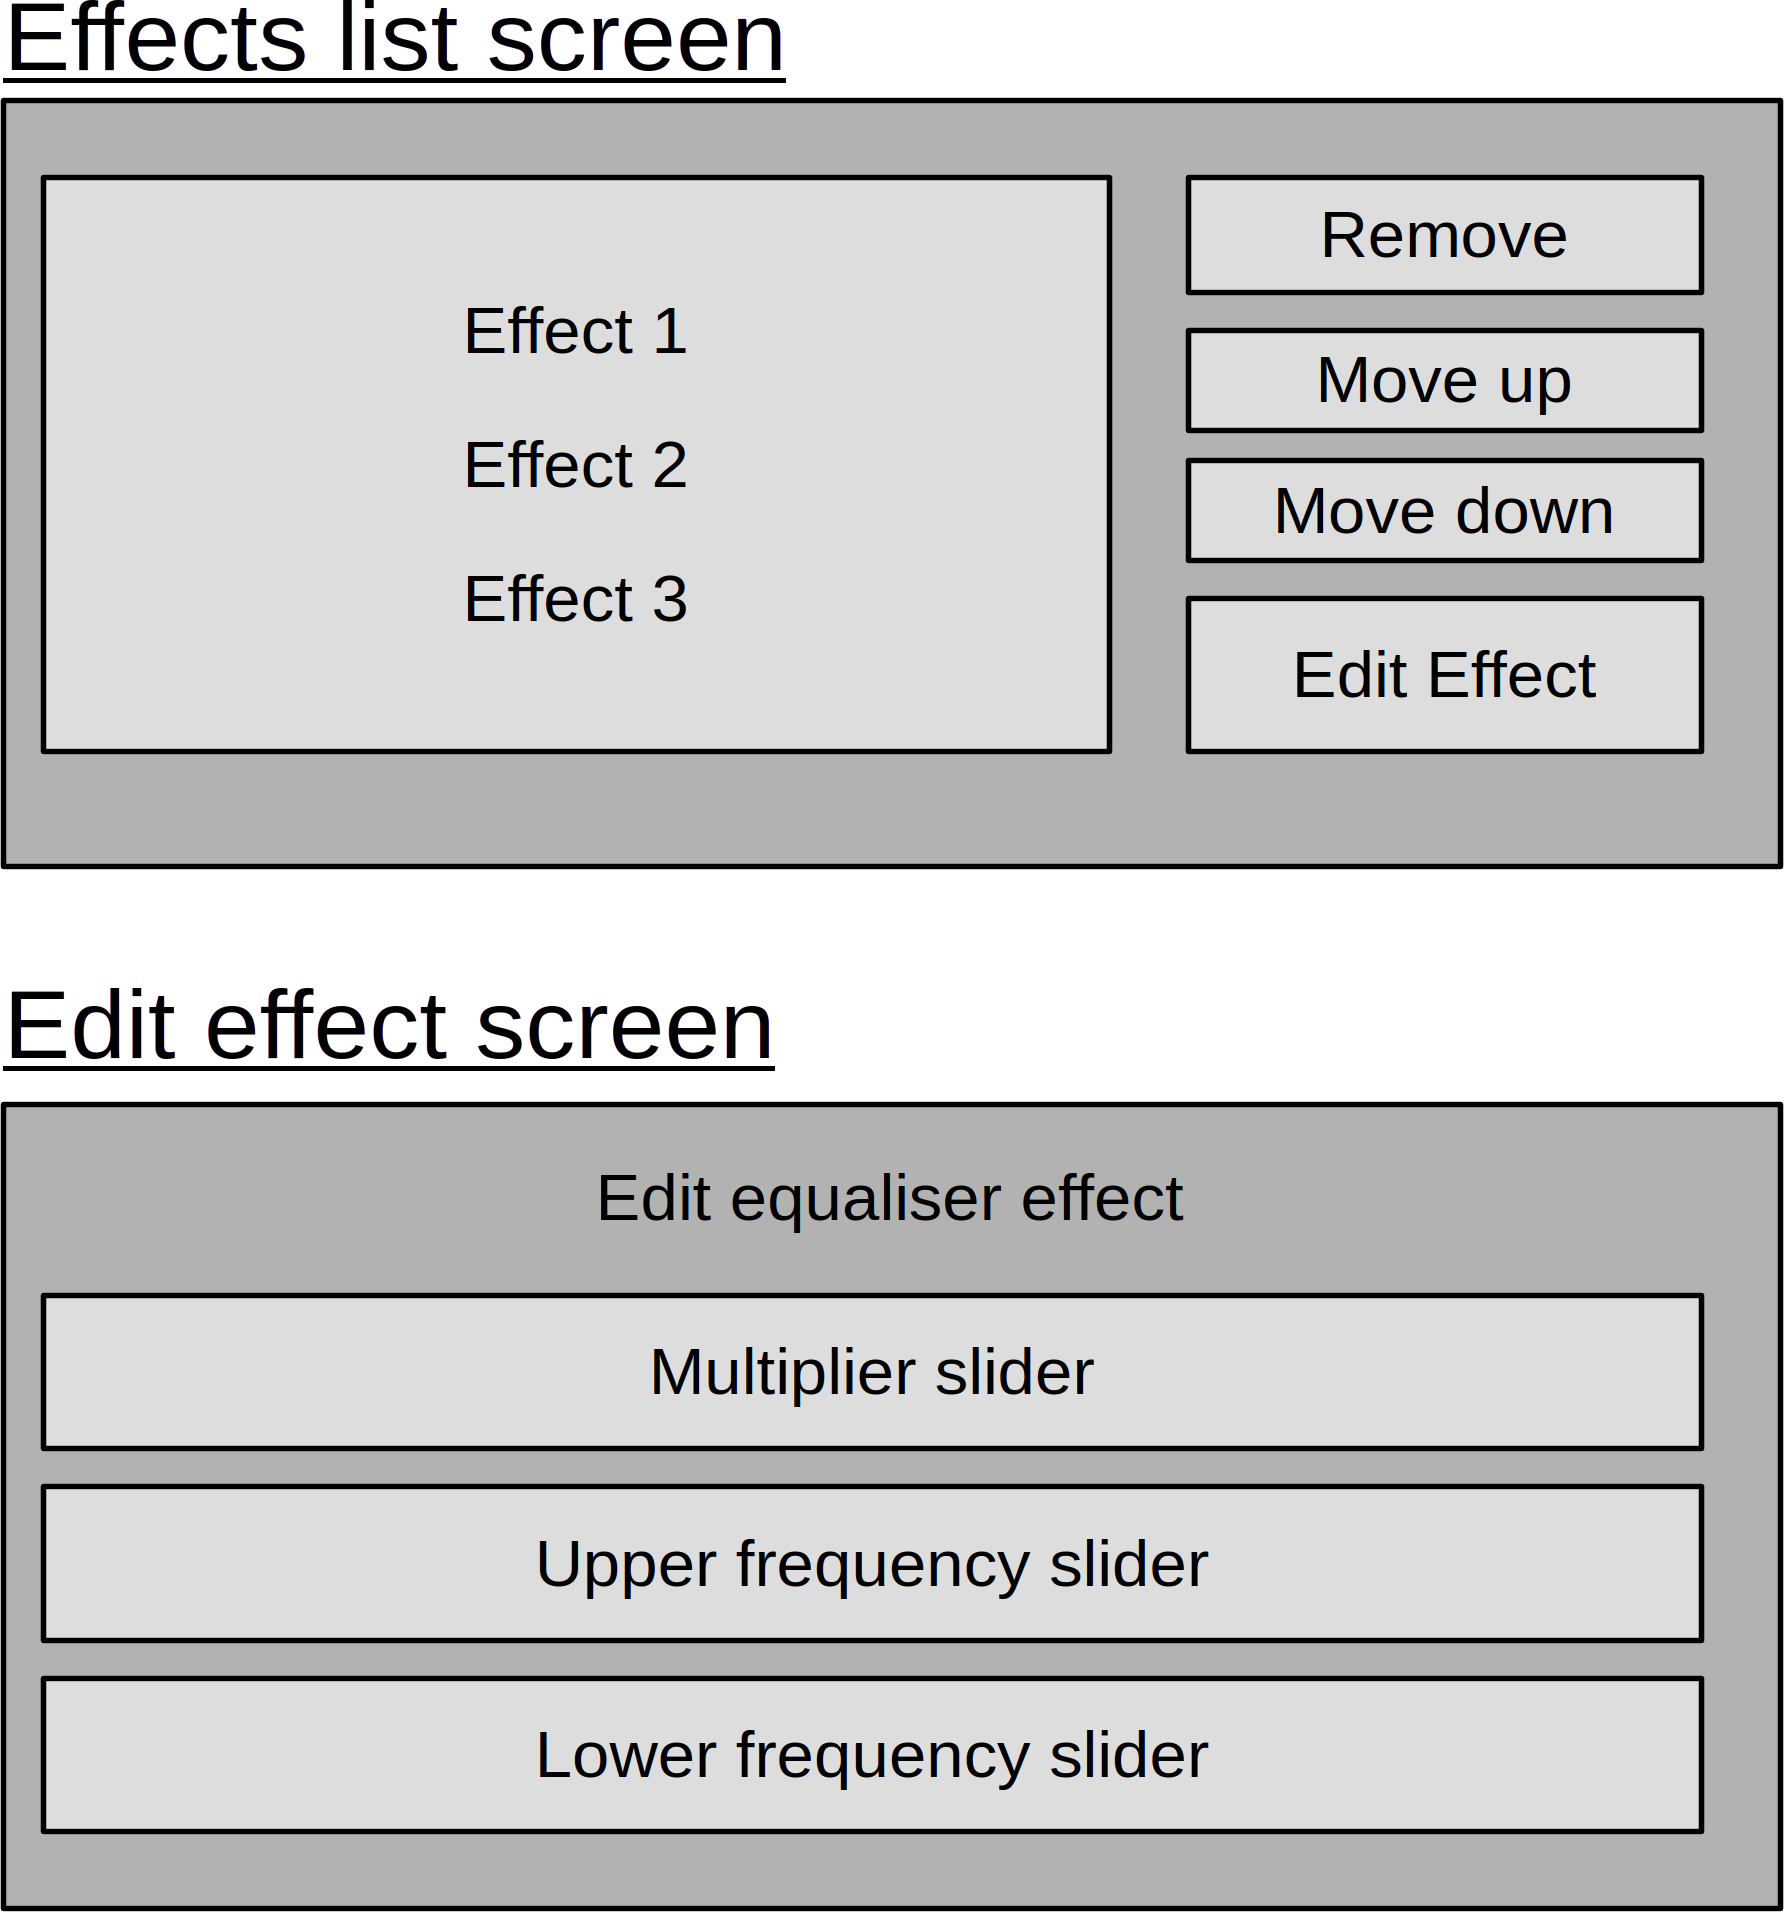
\includegraphics[width=14cm]{./gui wireframes two.png}
	\caption{GUI wireframes for ancillary windows }
\end{figure}

\subsubsection{Relation to the Code}
As I am using "wxWidgets" (see above), all GUIs must be programmed directly in code. I have decided, therefore, to create the following classes to abstract away the details of the GUI:
\begin{itemize}
	\item StartupWindow - implements the initial "choice screen"
	\item PlaylistWindow - implements the "create playlist screen"
	\item FileBrowser - responsible for fetching and drawing the  list of audio files on the system (used by PlaylistWindow). This is abstracted away as "wxWidgets" does not provide a native "widget" for this, so I must create my own.
	\item PlayWindow - implements the "playback screen"
	\item EffectsWindow - implements the "effects list" screen
	\item PropertiesWindow - implements the "edit effect" screen
	\item SongSelectionWindow - draws the popup for when the user chooses to select a new song from the current playlist (abstracted as is non-trivial to implement)
\end{itemize}

\pagebreak
\subsection{Defensive Programming}

\subsubsection{Reading and Writing Audio Files and Playlists}
\paragraph{}
Naturally the program has a need to consume data in various forms. There are three key filesystem operations:
\begin{itemize}
	\item Saving user-created playlists to disk
	\item Loading user-created playlists
	\item Loading audio files from disk
\end{itemize}

\paragraph{}
It should be stressed that any one of these operations could fail. A great many number of edge cases exist:
\begin{itemize}
	\item Upon loading a playlist, one or more audio files referenced may not actually exist
	\item An audio file may be unable to be loaded
	\item The user may lack sufficient permissions to save a playlist to a particular folder (e.g. /root)
	\item The user may input an invalid path when trying to load a playlist
\end{itemize}

\paragraph{}
Thus there is a need to carefully design IO-related subroutines so that, upon the event of failure, the program does not crash or behave incorrectly.

\paragraph{Loading Playlists}
\begin{enumerate}
	\item Upon a playlist file being selected, check it actually exists and can be read
	\item Read the file line by line (where each line corresponds to a path for an audio file)
	\item Verify each audio file actually exists on the system
	\item If an audio file is invalid or cannot be read, further defensive programming (described below when loading audio files themselves) will be employed.
\end{enumerate}

\paragraph{Loading Audio Files}
\begin{enumerate}
	\item When an audio file is loaded by the program (as it's about to be played), raise an exception if, for whatever reason, SDL cannot parse the audio file\footnote{
		Recall that SDL is being used as an audio library to load WAV files. SDL will return an error
		code if it fails, which may occur if the file is corrupt.
	}.
	\item Catch this exception in a try-catch block in the relevant GUI code.
	\item Remove the offending audio file from the playlist \textit{in memory} (not on the filesystem).
	\item If there are other audio files in the playlist, notify the user then skip to them instead (i.e. go to step 1 again).
	\item However if no valid audio files can be found, the entire playlist is invalid. Notify the user then terminate the program.
\end{enumerate}

\paragraph{Saving Playlists}
\begin{enumerate}
	\item Attempt to save the playlist file at the location the user specified.
	\item If the operation returned an error code, inform the user. Due to the control flow of the GUI, there is no need to further alter program flow\footnote{
		This is because the user saves playlists in the "create playlist" window. Once they click save, the window closes, and they are back at the screen presenting them with a choice to load an existing playlist or create a new one, regardless of whether or not the process succeeded. Hence all we need to do is notify the user if something went wrong.
	}.
\end{enumerate}

\subsubsection{Changing Audio Effect Properties}
\paragraph{}
Recall that each audio effect property has a minimum and a maximum value as defined in my UML class diagrams. These will be set explicitly in the code, so that a user cannot, for example, set the "volume property" in the volume effect to a negative number or chose a frequency in the equaliser effect that is outside the range of human hearing.

\paragraph{}
When the relevant GUI sliders are created to allow these properties to be changed, they must have their minimum and maximum values set respectively. This will ensure it is impossible to input invalid settings.

\pagebreak
\subsection{Audio Effect Presets}
\paragraph{}
Presets were idenitifed a key objective in the analysis section, due to the responses received in interviews. The aim is to allow a new user of the software to quickly reach a desired effect, lowering the barrier of entry, whilst also providing an opportunity to showcase how a range of effects can be combined for a particular purpose.

\paragraph{}
I will therefore add a variety of presets to my application, which showcases all of the audio effects at play. To this end I have designed the following presets:
\begin{itemize}
	\item "Far away room" - will apply an echo to make audio sound as if it's coming from a large room, before also applying an equaliser effect to limit higher frequencies\footnote{
		When sound waves are reflected, lower frequencies are typically reflected more readily than higher frequencies. For example, picture one's self a considerable distance from a party. Typically the bass can still be heard, as well as faint echoes of the vocals, but the higher frequencies have been drowned out as they have not been reflected so readily.
	}.
	\item "Spacious room" - as above, but will instead limit lower frequencies instead\footnote{
		This will make audio sound as if it's being played in a large hall or shopping centre, in which the audio echoes and sounds "tinny" on account of higher frequencies being muffled when reflected due to the materials used in construction.
	}.
	\item "Lo-fi" - Lo-fi refers to a popular genre of remixes in which song are made more "relaxing" by modifying the frequencies present and altering the speed of audio. Sometimes noise is also added.
	\item "Remove bass" - will use the equaliser effect to remove the bass from music.
	\item "Remove treble" - as above, but with treble
	\item "Low-quality speakers" - some people enjoy listening to "lower quality" versions of songs as they find it nostalgic. I will use the equaliser effect to reduce the range of frequencies heard, simulating a low-quality speaker, whilst also adding a small amount of echo and noise to enhance the effect.
\end{itemize}

\paragraph{}
By adding the above effects, many popular "genres" can be accounted for. In addition, all supported audio effects can be showcased to new users in an intuitive way.

\paragraph{}
I have decided to model presets using a functional approach, where each preset is a function, called within the program, that will apply and configure the particular effects required. However, it is unwise to specify, at this point in time, the exact parameters of these presets, as without first having writing the software, one cannot know how for certain how configuration options will behave. Yet broadly speaking, I believe a list of \textit{Preset} structures can be defined, each with a name, speed modifier\footnote{
	The Lo-fi preset will change the speed of audio playback, so I would do well to include this in the preset definition.
} and corresponding function.

\pagebreak
\subsection{Test Design}
\paragraph{}
In order to meet the objectives described in the analysis section, I have decided to design a variety of measurable tests which will indicate if these objectives have been met.
\textbf{For convenience, the objectives from above are repeated below:}

\paragraph{}
{
	\centering
	\fbox{\begin{minipage}{15cm}

			\begin{enumerate}
				\item  The user must be able to load a collection of audio files known as a "playlist" and then play the audio files contained within in a logical order
				\item  The user must be able to visualise the current audio being played in the frequency domain (i.e. visualise the frequencies)
				\item The user must be able to modify the audio's frequency domain (i.e. selectively modify frequencies such as by reducing the bass)
				\item The user must be able to apply additional "audio effects" to further enhance the music: echo, volume adjustment and noise
				\item The user must be able to configure these "audio effects" individually and also apply pre-made "presets" to quickly reach a desired effect
				\item  The system must run in real-time on an average school computer
			\end{enumerate}

	\end{minipage}}
}

\pagebreak
\subsubsection{Testing Objective 1}
\paragraph{Description} "The user must be able to load a collection of audio files known as a "playlist" and then play the audio files contained within in a logical order"

\paragraph{Test 1.1}
The user must have the option to create a new playlist from a list of audio files on the system.  To test this, I will therefore place a variety of audio files on disk and verify they are detected by the program. Non-audio files will not be able to be selected, for obvious reasons. As the only audio file currently supported is the ".wav" format, any file without this extension will not be displayed.

\paragraph{Test 1.2}
I will then test if playlists created in the program can be successfully saved to disk, then loaded back into the program in a sanitised manner. In other words, playlists consisting solely of files which actually exist on disk should be loaded without error (such that audio playback starts), but playlists with non-existent audio files should fail to load and notify the user of the error.

\paragraph{Test 1.3}
After loading a playlist and beginning audio playback, the audio files contained within must appear alphabetically in the audio file selection screen, ordered in ascending order by their respective filenames.

\paragraph{Test 1.4}
Any invalid audio files should be skipped over, and should not crash the program. The user should be notified if this happens.

\pagebreak
\subsubsection{Testing Objective 2}
\paragraph{Description} "The user must be able to visualise the current audio being played in the frequency domain (i.e. visualise the frequencies)"

\paragraph{}
As it is difficult for humans to visualise the frequency domain of audio themselves, I will generate audio files consisting of a sine wave of a constant, known frequency. Thus, when the frequency domain is visualised, there should be a single visual peak corresponding to the chosen frequency. By testing the visualisation in this manner across a range of frequencies, it should therefore be possible to deduce if the visualisation is correct.

\paragraph{}
Obviously the vast majority of audio being played will consist of multiple frequencies. I will therefore combine multiple sine waves in a single audio file (e.g. 500 Hz and 1000 Hz, both playing at the same time). Thus there should be multiple identifiable peaks, each one corresponding to a sine wave frequency chosen.

\paragraph{}
It should be stressed that human hearing only extends from 20 Hz to 20,000 Hz, and as such any audio visualisation must exclude frequencies outside these ranges.

\begin{figure}[H]
	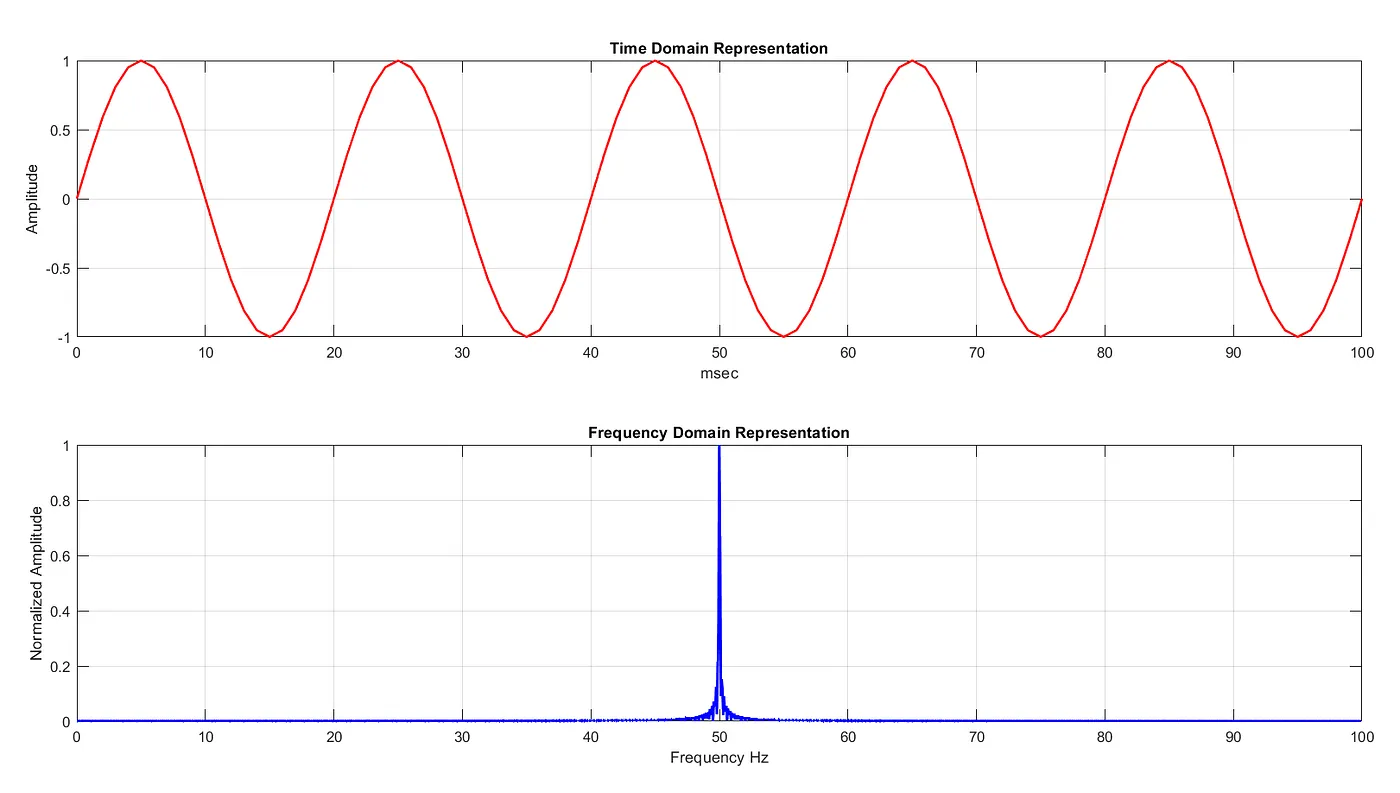
\includegraphics[width=14cm]{./fft test example.png}
	\caption{An example piece of audio, with the time domain shown above and the frequency domain below. If my tests succeed, they should look similar to the first picture (multiple sine waves will of course have multiple peaks of this nature). }
	% Credit - Aniket Kamat: https://aniket-kamat.medium.com/demystifying-the-fourier-transform-a995bdb6d73a
\end{figure}

\begin{multicols}{2}
\paragraph{Test 2.1} A correct visualisation of a sine wave is apparent at 500 Hz, with a single peak corresponding to that frequency.
\paragraph{Test 2.2} A correct visualisation of a sine wave is apparent at 1,000 Hz, with a single peak corresponding to that frequency.
\paragraph{Test 2.3} Sine waves outside the human audible range, at 10 Hz and 30,000 Hz respectively, produce no visible output, as they are inaudible.
\paragraph{Test 2.4} A correct visualisation of two sine waves (one at 1,000 Hz and one at 10,000 Hz) is apparent, with two separate peaks corresponding to those frequencies.
\paragraph{Test 2.5} A correct visualisation of three sine waves (1,000 Hz, 5,000 Hz and 15,000 Hz ) is apparent, with three separate peaks corresponding to those frequencies.
\end{multicols}

\pagebreak
\subsubsection{Testing Objective 3}
\paragraph{Description} "The user must be able to modify the audio's frequency domain (i.e. selectively modify frequencies such as by reducing the bass)"

\paragraph{Test 3.1}
The program's equaliser effect is able to selectively reduce the bass of any given audio (corresponding to the low frequencies in frequency space).

\paragraph{Test 3.2}
The program's equaliser effect is able to selectively reduce the treble of any given audio (corresponding to the high frequencies in frequency space).

\paragraph{Verifying Results}
I will verify the results both by ear and using the audio visualiser\footnote{
	For example, if one chooses to reduce the bass, then the parts
	of the visualisation corresponding to the lower frequencies must
	visually appear smaller in relation to the other frequencies.
}, so as the ensure that the program is able to selectively reduce the range of frequencies chosen.

\pagebreak
\subsubsection{Testing Objective 4}
\paragraph{Description} "The user must be able to apply additional "audio effects" to further enhance the music: echo, volume adjustment and noise"

\paragraph{}
Due to the subjective nature of audio effects, I will ask multiple people from the program's target audience to provide in-depth feedback on all the audio effects.

\paragraph{}
Recall that the goal of this project is to assist in the user-friendly and convenient creation of song remixes, and so I will ask them to verify that the audio effects produced by the program mimic the effects typically heard in said remixes.

\paragraph{}
At least one of these people will be someone experienced in audio processing, so that they are able to assess if the effects provided sound physically accurate
(particularly the echo). I plan on using my Maths teacher Mr Godwin for this (referred to in later sections as the "Subject Specialist"), as he has experience in Digital Signal Processing (particularly as it relates to audio) from his university degree in Maths, and has a keen ear for audio. He also has experience in sound production at live events, so will be knowledgeable about what a correct echo will sound like.

\paragraph{Test 4.1} A select group from the target audience certify that the echo effect sounds physically plausible, and mimics the effect as it is commonly heard in song remixes
\paragraph{Test 4.2} A select group from the target audience certify  that the noise effect sounds physically plausible, and mimics the effect as it is commonly heard in song remixes
\paragraph{Test 4.3} The volume effect can be seen to adjust the volume correctly

\pagebreak
\subsubsection{Testing Objective 5}
\paragraph{Description} "The user must be able to configure these "audio effects" individually, yet also apply pre-made "presets" to quickly reach a desired effect"

\paragraph{Test 5.1} The noise effect can have its various parameters modified, which results in a correct change in the audio playback.
\paragraph{Test 5.2} The echo effect can have its various parameters modified, which results in a correct change in te audio playback.
\paragraph{Test 5.3} The equaliser effect can have its various parameters modified, which results in a correct change in the audio playback.
\paragraph{Test 5.4} All presets present in the application can be loaded successfully, with the appropriate audio effects having been added and configured correctly, such that the desired effect is reached.

\paragraph{}
There is no need to test the volume effect here, as configuring it was already covered in test 4.3.

\pagebreak
\subsubsection{Testing Objective 6}
\paragraph{Description}  "The system must run in real-time on an average school computer"

\paragraph{}
I will test the performance of the program by running it on a computer in my school, which represents more-or-less average hardware.
I will also test it on my school laptop too, which has more modest hardware, to ensure that in all contexts in which a student might run the program, there will be no performance issues.
In order to appear to run in real-time, the following must be observed:
\begin{enumerate}
	\item The audio  playback must not slow down \footnote{If audio processing takes too long, then the audio callback will be called less frequently than the hardware demands, resulting
		in a very noticeable slowdown. This must not happen.}.
	\item The visualisation graphics must update in less than 16.6 ms, such that it is displayed at 60 FPS, which is the most common refresh rate on school hardware. This will be measured by
	the code itself as it's running.
\end{enumerate}

\paragraph{Test 6.1} The program must run, without any effects applied, in real-time on the specified hardware
\paragraph{Test 6.2} The program must run in real-time, for every preset applied separately, in real-time on the specified hardware.
\paragraph{Test 6.3} The program must run in real-time, with every effect applied at once, in real-time on the specified hardware.

\pagebreak
\subsection{Final overview of project hierarchy}
\begin{figure}[H]
	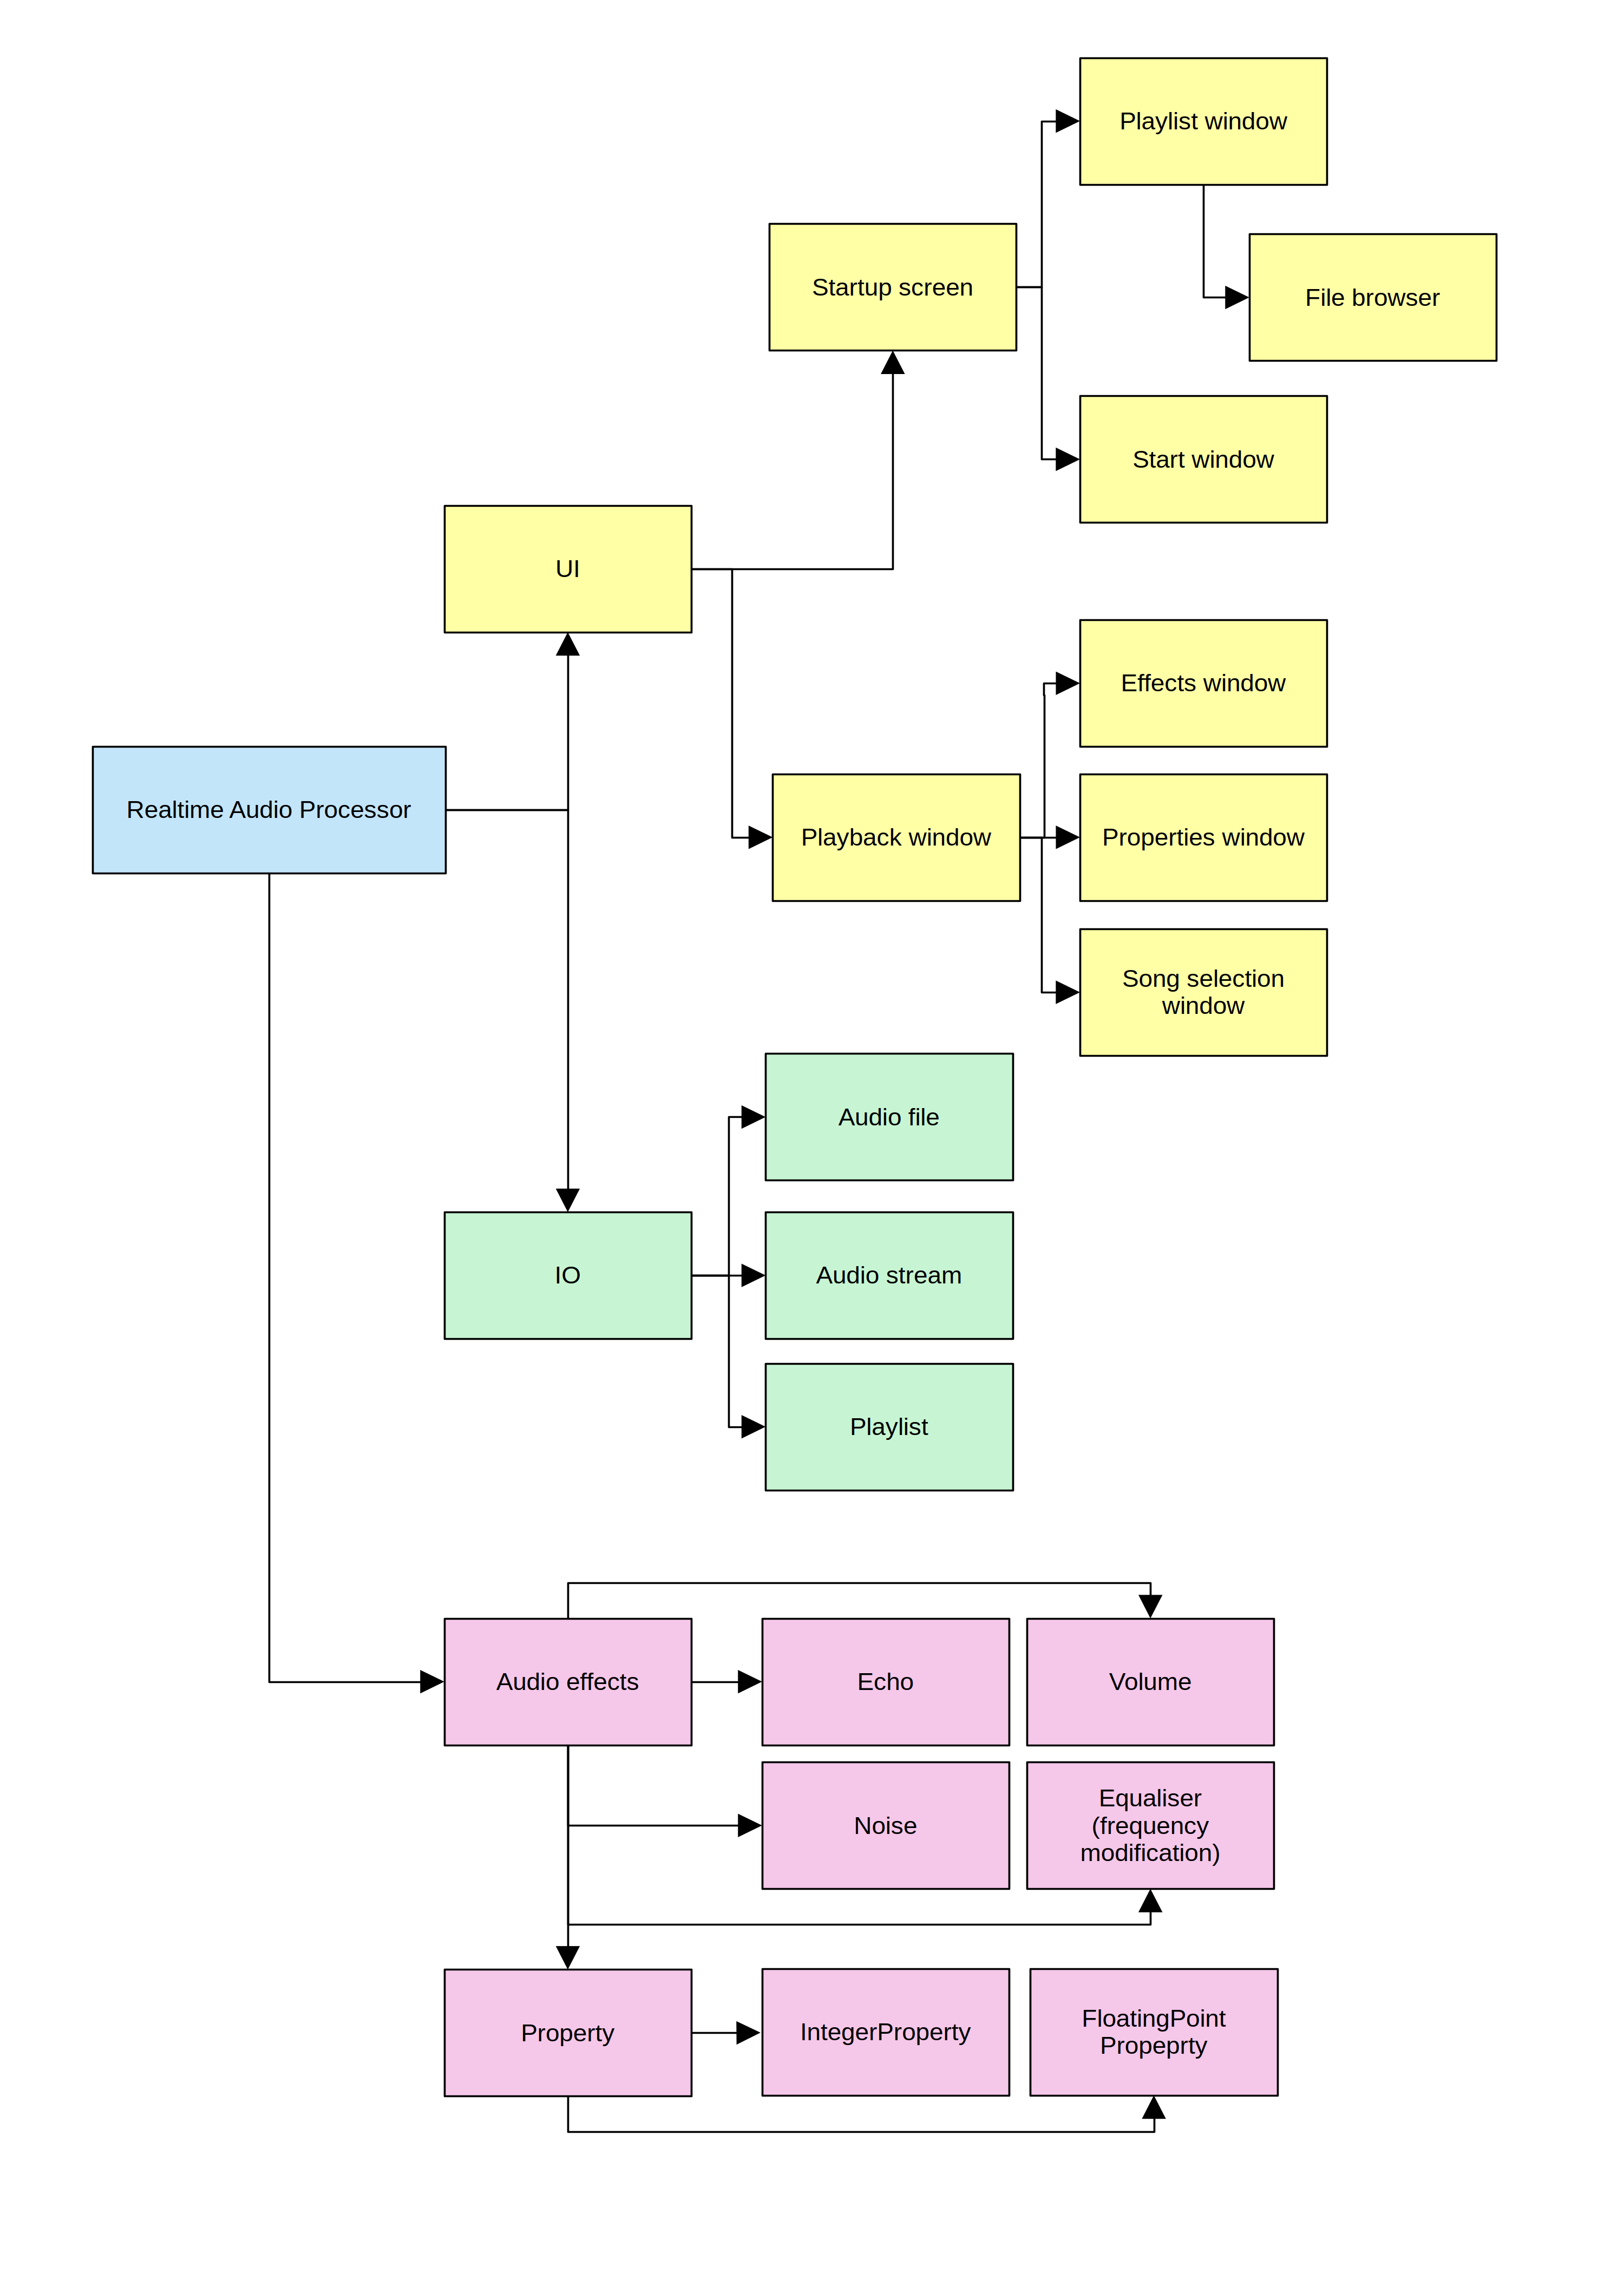
\includegraphics[width=14cm]{./hierarchy chart.png}
	\caption{Hierarchy chart }
\end{figure}

	\section{Development and Implementation}

Whilst the full source code is available in the appendix, the following section contains the most important parts of the code-base, highlighting the techniques used and technical solutions employed.

\subsection{Summary of techniques}
For handy reference, below is a table summarising the various techniques used in the codebase. \textbf{These are expanded upon in more detail below}.

{
	\renewcommand{\arraystretch}{1.5}
	\begin{table}[h!]
		\begin{center}
			\begin{tabularx}{1.0 \textwidth} {
					| >{\raggedright\arraybackslash}X 
					| >{\raggedright\arraybackslash}X
					| >{\raggedright\arraybackslash}X 
					|
				}
				\hline
				Source File & Technique & Purpose \\
				
				\hline
				include/data/atomic\_linked\_list.h & Thread-safe linked list (including linked list maintenance) from scratch and use of function callbacks & Provides data structure for inter-thread communication (see section 2.1) \\
				
				\hline
				include/data/tree.h and src/ui/file\_browser.cpp & Tree data structure and recursive navigation of filesystem & Used in file browsing to represent filesystem structure and allow the user to browse for audio files \\
				
				\hline
				src/data/merge-sort.cpp & Recursive merge-sort  algorithm implementation & To sort playlist files alphabetically \\
				
				\hline
				src/effects/fft.cpp & Cooley-Tukey Fast Fourier algorithm implementation & To aid in audio procession and visualisation \\
				
				\hline
				src/ui/audio\_visualiser.cpp & Uses FFT data & Renders audio visualisation \\
				
				\hline
				include/effects/audio\_effect.cpp & Polymorphic "audio effect" base class (inherited by children) - including use of hashmap & Manages common interface \\
				
				\hline
				include/effects/*property.h & Polymorphic "property" base class and associated children & Provides common interface for setting and getting properties of different types \\
				
				\hline
				src/effects/echo\_effect.cpp & Inheritance & Echo effect implementation \\
				
				\hline
				src/effects/equaliser\_effect.cpp &  Inheritance and use of Fourier algorithms & Audio equaliser implementation \\
				
				\hline
				src/effects/noise\_effect.cpp & Inheritance & Noise effect implementation \\
				
				\hline
				src/effects/volume\_effect.cpp & Inheritance & Volume effect implementation \\
				
				\hline
				Various files & Use of function callbacks & Used in many places, including preset creation and UI code \\
				
				\hline
				Various files & Error handling and user input sanitisation & Prevent program from experiencing crashes, security issues and undefined behaviour \\
				
				\hline
			\end{tabularx}
		\end{center}
	\end{table}
}

\pagebreak
\subsection{Atomic Linked List - \textit{include/data/atomic\_linked\_list.h}}
As discussed in section 2, the atomic linked list is a crucial component of the project.  It makes use of generics (C++ "templates") to allow it to store any arbitrary data type. 

The full code is listed below, followed by explanations below of the most critical parts.

\inputminted[linenos]{c++}{../include/data/atomic_linked_list.h}

\paragraph{Mutexes} Whenever a caller accesses the data structure, the mutex is first locked. The relevant operation is then performed, and the mutex is then unlocked, freeing the data structure for future use (in this thread or otherwise). This can be seen in the functions Add, Remove, ForEach, SwapWithNext and Reset.

\paragraph{Generics} To make the data structure as flexible as possible, it is written to store a generic type "T". Note that we cannot store a variable of type T directly, but must rather store a pointer to each "T", as some types may be too big to store on the stack.

\paragraph{Callbacks} The data structure provides a "ForEach" method which takes a callback as an argument. This callback is invoked upon every node in the linked list, in order to allow for arbitrary operations to be formed on each element. This is used in \textit{src/io/audio\_stream.cpp} and \textit{src/ui/effects\_window.cpp} to iterate over each node. For example, in the \textit{AudioStream} class:
\begin{minted}{c++}
effects->ForEach([&](AudioEffect* effect) {
	effect->ApplyEffect(packet);
});
\end{minted}

\paragraph{Linked List Maintenance}  The head and tail pointers of affected nodes are updated when adding and removing a node (in the \textit{Add} and \textit{Remove} subroutines respectively), as well as when swapping two nodes (\textit{SwapWithPrevious} and \textit{SwapWithNext}). The head and tail pointers are then used when iterating over the list (for example in \textit{ForEach}), and when calling the destructor.


\pagebreak
\subsection{File Browser and Associated Tree - \textit{include/data/tree.h} and \textit{src/ui/file\_browser.cpp }}

The filesystem is inherently recursive - that is, folders may contain files, but also other folders, which may themselves contain other files and folders. In order to elegantly model this, I decided to use a recursive tree. This resulted in the ability to represent, in memory, the exact nature of the filesystem, allowing for the GUI display below:

\begin{figure}[h]
	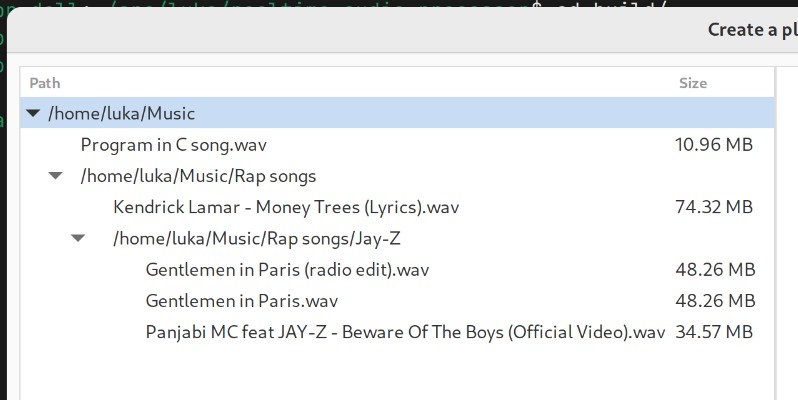
\includegraphics[width=13cm]{./file browser demo.png}
	\caption{Audio files are displayed in a graphical tree, backed by a tree in memory}
\end{figure}

\subsubsection{Tree data structure - \textit{include/data/tree.h}}
First, it was necessary to implement a tree data structure. Each node has a piece of data, followed by a list pointers to child nodes. Each child node may itself contain a piece of data, and a list of its own children.

As in C++ one must free explicit heap allocations manually,  recursion had to be used in the destructor. When the root node is destroyed, the following process occurs:
\begin{enumerate}
	\item C++ will call the destructor of the tree
	\item The tree iterates through all its children and calls their own respective destructors (line 16)
	\item This process repeats recursively until all children have deallocated their own children, and then finally themselves.
	\item Finally the root node deallocates itself.
\end{enumerate}
The full code is listed below.
\pagebreak
\inputminted[linenos]{c++}{../include/data/tree.h}

\pagebreak
\subsubsection{File Browser - \textit{src/ui/file\_browser.cpp}}
The file browser uses the tree data structure to store its files, and uses recursion to a greater extent. Below are the relevant parts of the code, followed by a description.

\inputminted[linenos, firstline=47, lastline=108]{c++}{../src/ui/file_browser.cpp}

\paragraph{The \textit{ScanDirectory} subroutine} This function is called on the root audio file directory (the user's Music folder). It creates a tree with a single node, containing the path to this directory. It then iterates through all the files and folders in the root directory. Files are added as children of the root node. If a directory is encountered instead, a tree for that directory is created by recursively calling \textit{ScanDIrectory} again, which is then added as a child to the existing tree. In this way, all files and folders contained within the root directory are added.  

\paragraph{The \textit{AddDirectory} subroutine} This subroutine is called once the tree containing all files and folders has already been created in \textit{ScanDirectory}. Each element is recursively added to a \textit{wxTreeListCtrl} (for the purposes of displaying the tree in the GUI) by first adding the directory itself, followed by the files contained within, then adding the sub-directories, which is done by recursively calling the function.

\pagebreak
\subsection{Merge Sort - \textit{src/data/merge\_sort.cpp}}
For ordering playlists alphabetically, a sorting  algorithm was needed. I decided to use a merge sort due to its low time complexity of \(O(N \log{N})\).
\inputminted[linenos]{c++}{../src/data/merge_sort.cpp}

\pagebreak
\subsection{Fourier Processing - \textit{src/effects/fft.cpp}}
This implements the pseudo-code produced in section 2.5, and hence uses recursion and the relevant Fourier maths, as well as linearising frequencies using the Bark scale. The relevant code is contained below.

\subsubsection{FFT Algorithm}
\inputminted[linenos, firstline=1, lastline=79]{c++}{../src/effects/fft.cpp}

\pagebreak
\subsubsection{Visualisation Algorithm}
As discussed in section 2.5, this transforms the data into a format easily plottable by the GUI code, and takes into account the non-linear scale of human hearing.
\inputminted[linenos, firstline=81, lastline=148]{c++}{../src/effects/fft.cpp}

\pagebreak
\subsubsection{Corresponding code to draw in GUI - \textit{src/ui/audio\_visualiser.cpp}}
Initially, results from the FFT were plotted straight to the screen. However, a key issue arose: audio changed so rapidly between frames that any visualisation was too flickery to be useful or readable.  To solve this, it was necessary to average the results of the FFT over multiple frames, so that changes in frequencies appeared more gradually. I also decided to colour the bars in the bar chart in accordance with their frequencies in order to increase the readability of the visualisation.

Each time a fixed buffer of audio is fed to the audio device (i.e. played to the speakers), the \textit{FeedAudio} subroutine is called, which performs a Fourier transform, adds it to the list of previous results for averaging, then triggers a GUI refresh.
\inputminted[linenos, firstline=15, lastline=44]{c++}{../src/ui/audio_visualiser.cpp}
\inputminted[linenos, firstline=67, lastline=156]{c++}{../src/ui/audio_visualiser.cpp}

\pagebreak
\subsection{Audio Effects and Properties}

\subsubsection{Base Audio Effect Class - \textit{include/effects/audio\_effect.h}}
The \textit{AudioEffect} base class has three key features:
\begin{enumerate}
	\item Provides a common interface for accessing "properties" (such as effect intensity). These properties are stored in a hashmap so that the names of the properties can be used as keys, and so that properties can be looked up with constant time complexity, which is important if any audio effects are added in the future that have a large number of properties to avoid wasting CPU cycles.
	\item Provides a common interface to identify the name of an effect in the GUI
	\item Provides a common interface to apply the effect to a "packet" of audio
\end{enumerate}
\inputminted[linenos]{c++}{../include/effects/audio_effect.h}

\pagebreak
\subsubsection{Property Base class - \textit{include/effects/property.h}}
\inputminted[linenos]{c++}{../include/effects/property.h}

\pagebreak
\subsubsection{IntegerProperty - \textit{include/effects/integer\_property.h}}
\inputminted[linenos]{c++}{../include/effects/integer_property.h}

\pagebreak
\subsubsection{FloatingPointProperty - \textit{include/effects/floating\_point\_property.h}}
\inputminted[linenos]{c++}{../include/effects/floating_point_property.h}




	\section {  Testing }

	\section {  Evaluation }

	\section { Appendix  }

	\subsection{Copy of Interview Questionnaire}

	{
	\centering
	\fbox{\begin{minipage}{15cm}
			\begin{center}
			{\huge Luka's Questionnaire Form}
			\end{center}

			For my A-level Computer Science coursework  I am writing a program that allows users to easily apply various audio effects to songs, in order to make experimenting with music and creating remixes easier. In order to create the best possible software, I would like your opinion on what makes a remix good. Please answer the questions below in a concise and understandable manner, then email me your responses.

			\paragraph{Questions}
			\begin{enumerate}
				\item Why do you sometimes prefer a song's remix?
				\item How does a remix typically differ from the original song?
				\item What features would you like in a real-time audio editing program to assist in "remixing" music?
			\end{enumerate}
	\end{minipage}}
}


	\section { Code example }
		\begin{minted}{c++}
void EqualiserEffect::ModifySamples(std::vector<float>& samples, const float frequency) const
{
	// Perform FFT to convert to frequency domain
	FastFourierTransform fft(samples, std::nullopt);
	std::vector<std::complex<float>>& fft_output = fft.output;

	ModifyFrequencies(fft_output, frequency);

	// Perform IFFT to convert back to time domain
	InverseFourierTransform inverse(fft_output);
	std::vector<float> scaled_real_components;
	scaled_real_components.reserve(samples.size());
	for (const auto& c : inverse.output)
		scaled_real_components.emplace_back(
			c.real() / (float)inverse.output.size()
		);

	samples = scaled_real_components;
}
	\end{minted}
	
	\subsection{TODO}
	\begin{itemize}
		\item design tests in the design
		\item narritive: testing: test passed/failed, opinions from others on effects
		\item evaluation: use testing to say if objectives passed
		\item evaluation: obejctives pass, but was overall project aim met?
		\item talk about merge sort
		\item talk about atomic linked list
		\item talk about tree
		\item "fisher yates" shuffle
	\end{itemize}
	

\end{document}